\documentclass[UTF8,11pt]{article}

  % Package for using the full page.
  \usepackage{fullpage}
  
  % Package for writing algorithms (why do we need this one?).
  \usepackage[linesnumbered,ruled,vlined]{algorithm2e}
  
  % Package for using colored texts.
  \usepackage[pdftex,dvipsnames]{xcolor}
  
  % Pakcage for using multiple optional parameters in new commands.
  \usepackage{xargs}

  % Packages for writing comments and todo notes.
  \usepackage[colorinlistoftodos,prependcaption,textsize=tiny]{todonotes}
  \newcommandx{\unsure}[2][1=]
    {\todo[linecolor=red,backgroundcolor=red!25,
	bordercolor=red,#1]
	{#2}\xspace{}}
  \newcommandx{\change}[2][1=]
    {\todo[linecolor=blue,backgroundcolor=blue!25,
	bordercolor=blue,#1]
	{#2}\xspace{}}
  \newcommandx{\info}[2][1=]
    {\todo[linecolor=OliveGreen,backgroundcolor=OliveGreen!25,
	bordercolor=OliveGreen,#1]
	{#2}}
  \newcommandx{\improvement}[2][1=]
    {\todo[linecolor=Plum,backgroundcolor=Plum!25,bordercolor=Plum,#1]
	{#2}\xspace{}}
  \newcommandx{\thiswillnotshow}[2][1=]
    {\todo[disable,#1]
	{#2}\xspace{}}

  % What are there for?
  % Select what to do with todonotes: 
  % \usepackage[disable]{todonotes} % notes not showed
  % \usepackage[draft]  {todonotes} % notes showed

  % Select what to do with command \comment:  
  % \newcommand{\comment}[1]
      {}                                    %comment not showed
  \newcommand{\comment}[1]
    {\par {\bfseries \color{blue} #1 \par}} %comment showed
  
  % ams math packages.
  \usepackage{amsmath, amssymb, amsthm}
  
  % Declare a global counter for theorem environments:
  \newcounter{thmcounter}
  
  % Define new theorem styles and theorem environments.
  \theoremstyle{plain}
  
  \newtheorem{theorem}    [thmcounter]{Theorem}
  \newtheorem{corollary}  [thmcounter]{Corollary}
  \newtheorem{lemma}      [thmcounter]{Lemma}
  \newtheorem{proposition}[thmcounter]{Proposition}
  
  \theoremstyle{definition}
  
  \newtheorem{definition} [thmcounter]{Definition}
  \newtheorem{example}    [thmcounter]{Example}
  
  \theoremstyle{remark}
  
  \newtheorem{remark}     [thmcounter]{Remark}
  \newtheorem{notation}   [thmcounter]{Notation}
  
  
  % Package for changing fonts in the Verbatim environment:
  \usepackage{fancyvrb}
  
  % Package for writing captions for align environment:
  \usepackage{capt-of}
  
  % Package for URLs:
  \usepackage{hyperref}  
  
  % Package for tables:
  \usepackage[english]{babel}  
  
  % Package for quotations:
  \usepackage{csquotes}
  
  % Package for customizing lists environments:
  \usepackage{enumitem}
  
  % Package for writing long tables:
  \usepackage{longtable}
  
  % Package for graphics
  \usepackage{graphicx}
  
  % Define ceiling and flooring symbols:
  \usepackage{mathtools}
  \DeclarePairedDelimiter{\ceil}{\lceil}{\rceil}
  \DeclarePairedDelimiter{\floor}{\lfloor}{\rfloor}

  % Package for underlining and strikethrough texts.
  \usepackage[normalem]{ulem}
  
  % Package for display-mode quotations.
  \usepackage{csquotes}
  
  % Define double-bracket [[P]]
  \usepackage{stmaryrd}
  \newcommand{\Bracket}[1]{\llbracket#1\rrbracket}
  
  % Package for writing natural proof deductions
  \usepackage{prftree}
    
  % Package for writing BNF syntax
  \usepackage{syntax}
  
  % Package for lstlisting and definition of Kore
  \usepackage{listings}
  % Define colors
  \definecolor{codegray}{rgb}{0.5,0.5,0.5}
  \definecolor{backgray}{RGB}{250,250,250}
  \definecolor{codegreen}{RGB}{50,205,50}
  \definecolor{codeblue}{RGB}{50,50,255}
  % Define Kore Language style
  \lstdefinelanguage{kore}
  {
  	% print whole listing small and in serif fonts
  	basicstyle=\ttfamily\footnotesize,
  	% use /* */ for comments
  	morecomment=[s]{/*}{*/},
  	% print white for comments
  	commentstyle=\color{codegray},
  	% print line number in the left, in tiny fonts
  	numbers=left,
  	numberstyle=\tiny,
  	% print all characters at their natural width
  	columns=fullflexible,
  	% print background color grey
  	backgroundcolor=\color{backgray},
  	% regard some characters as letters
  	alsoletter={-\#\\},
  	% list of declaration keywords
  	keywordstyle=[1]\color{codeblue},
  	morekeywords=[1]{
  		module,
  		endmodule,
  		hooked-sort,
  		sort,
  		symbol,
  		hooked-symbol,
  		alias,
  		axiom,
  	},
    % list of connectives
    keywordstyle=[2]\color{codegreen},
    morekeywords=[2]{
    	\\not,
    	\\or,
    	\\implies,
    	\\and,
    	\\equals,
    	\\exists,
    	\\forall,
    	\\iff
    }
  }

  % Define |-fin
  \newcommand{\vdashfin}{\vdash_\text{fin}}

  % Define the colon ":" that is used in "x:s"
  % with less spacing around.
  \newcommand{\cln}{\texttt{:}}

  % Define the curly K:
  \newcommand{\K}{\mbox{$\mathbb{K}$}\xspace}
  
  % Define commands that are used in Sec 2.  
  \newcommand{\Nat}{\textit{Nat}}
  \newcommand{\KNat}{\textit{KNat}}
  \newcommand{\Int}{\textit{Int}}
  \newcommand{\Bool}{\textit{Bool}}
  \newcommand{\List}{\textit{List}}
  \newcommand{\KList}{\textit{KList}}
  \newcommand{\nil}{\textit{nil}}
  \newcommand{\cons}{\textit{cons}}
  \newcommand{\append}{\textit{append}}
  \newcommand{\Bag}{\textit{Bag}}
  \newcommand{\Set}{\textit{Set}}
  \newcommand{\Map}{\textit{Map}}
  \newcommand{\emptyMap}{\textit{empty}}
  \newcommand{\bindMap}{\textit{bind}}
  \newcommand{\mergeMap}{\textit{merge}}
  \newcommand{\ittrue}{\textit{true}}
  \newcommand{\itfalse}{\textit{false}}
  \newcommand{\itceil}{\textit{ceil}}
  
  \newcommand{\Pred}{\textit{Pred}}

  \newcommand{\Context}{\textit{Context}}
  \newcommand{\hole}{\boxempty}
  \newcommand{\Exp}{\textit{Exp}}
  \newcommand{\AExp}{\textit{AExp}}
  \newcommand{\BExp}{\textit{BExp}}
  \newcommand{\Stmt}{\textit{Stmt}}
  \newcommand{\ite}{\textsf{ite}}
  \newcommand{\ttrue}{\textit{true}}
  \newcommand{\ffalse}{\textit{false}}
  \newcommand{\app}{\textit{app}}
  \newcommand{\KExp}{\mathit{\#Exp}}
  \newcommand{\Klambdazero}{\mathit{Klambda0}}
  \newcommand{\Kapp}{\mathit{Kapp}}
  \newcommand{\Klambda}{\mathit{Klambda}}
  \newcommand{\parametric}[2]{{#1}\raisebox{.2ex}{\texttt{\footnotesize{\{}}}#2\raisebox{.2ex}{\texttt{\footnotesize{\}}}}}
  \newcommand{\parametricscript}[2]{{#1}\raisebox{.2ex}{\texttt{\tiny{\{}}}#2\raisebox{.2ex}{\texttt{\tiny{\}}}}}
  
  \newcommand{\zero}{\textit{zero}}
  \newcommand{\Kzero}{\textit{Kzero}}
  \newcommand{\Ksucc}{\textit{Ksucc}}
  \newcommand{\KSymbolsucc}{\textit{KSymbolsucc}}
  \newcommand{\Mod}{\textit{Mod}}
  \newcommand{\denote}[1]{\llbracket{#1}\rrbracket}
  \newcommand{\reduct}[2]{\mbox{${#1}\!\!\upharpoonright_{#2}$}}
  \newcommand{\reductscript}[2]{\mbox{\tiny${#1}\!\!\upharpoonright_{#2}$}}
  
  \newcommand{\isEmpty}{\textit{isEmpty}}
  
  \newcommand{\builtin}{\textit{builtin}}
  
  % Define PATTERNS with ATTERNS are small capitals:
  \newcommand{\PATTERNS}{\text{P\textsc{atterns}}}
  \newcommand{\VARIABLES}{\text{V\textsc{ariables}}}
  % Define sorts and symbols in the calculus K.
  
  \newcommand{\doubleslash}{/\!/{ }}
  

  \newcommand{\shp}{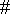
\includegraphics{hash-symbol}\kern-0.1em}
  \newcommand{\smallshp}{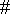
\includegraphics[scale=0.8]{hash-symbol}\kern-0.1em}
  \newcommand{\sharpsymbol}{\#}
  \newcommand{\shs}{\shp s}
  \newcommand{\smallshs}{\smallshp s}
  % Sec 3.1 Truth
  \newcommand{\KPred}{\mathit{\shp Pred}}
  
  % Sec 3.2 Strings
  \newcommand{\KChar}{\texttt{\sharpsymbol Char}}
  \newcommand{\KCharList}{\texttt{\sharpsymbol CharList}}
  \newcommand{\KString}{\texttt{\sharpsymbol String}}
  \newcommand{\Kepsilon}{\texttt{\sharpsymbol epsilon}}
  \newcommand{\KconsKString}{\texttt{\sharpsymbol consKString}}
  
  %% We shouldn't need the follows.  
  \newcommand{\Kconcat}{\texttt{\sharpsymbol concat}}
  
  % Sec 3.3 Sorts and Symbols
  \newcommand{\KSort}{\texttt{\sharpsymbol Sort}}
  \newcommand{\Ksort}{\texttt{\sharpsymbol sort}}
  \newcommand{\KSymbol}{\texttt{\sharpsymbol Symbol}}
  \newcommand{\Ksymbol}{\texttt{\sharpsymbol symbol}}
  \newcommand{\KSymbolceil}{\texttt{\sharpsymbol `ceil}}
  \newcommand{\KgetArgumentSorts}{\texttt{\sharpsymbol getArgumentSorts}}
  \newcommand{\KgetReturnSort}{\texttt{\sharpsymbol getReturnSort}}
  
  % Sec 3.4 Finite Lists
  \newcommand{\ttX}{\texttt{X}}
  \newcommand{\ttChar}{\texttt{Char}}
  \newcommand{\ttSort}{\texttt{Sort}}
  \newcommand{\ttSymbol}{\texttt{Symbol}}
  \newcommand{\ttVariable}{\texttt{Variable}}
  \newcommand{\ttPattern}{\texttt{Pattern}}
  \newcommand{\XList}{\texttt{\sharpsymbol XList}}
  \newcommand{\KnilXList}{\texttt{\sharpsymbol nilXList}}
  \newcommand{\KconsXList}{\texttt{\sharpsymbol consXList}}
  \newcommand{\KappendXList}{\texttt{\sharpsymbol appendXList}}
  \newcommand{\KinXList}{\texttt{\sharpsymbol inXList}}
  \newcommand{\KdeleteXList}{\texttt{\sharpsymbol deleteXList}}
  \newcommand{\KPatternList}{\texttt{\sharpsymbol PatternList}}
  \newcommand{\KnilKPatternList}{\texttt{\sharpsymbol nilPatternList}}
  \newcommand{\KconsKPatternList}{\texttt{\sharpsymbol consPatternList}}
  \newcommand{\KappendKPatternList}{\texttt{\sharpsymbol appendPatternList}}
  \newcommand{\KinKPatternList}{\texttt{\sharpsymbol inPatternList}}
  \newcommand{\KdeleteKPatternList}{\texttt{\sharpsymbol deletePatternList}}
  \newcommand{\KSortList}{\texttt{\sharpsymbol SortList}}
  \newcommand{\KnilKSortList}{\texttt{\sharpsymbol nilSortList}}
  \newcommand{\KconsKSortList}{\texttt{\sharpsymbol consSortList}}
  \newcommand{\KappendKSortList}{\texttt{\sharpsymbol appendSortList}}
  \newcommand{\KinKSortList}{\texttt{\sharpsymbol inSortList}}
  \newcommand{\KdeleteKSortList}{\texttt{\sharpsymbol deleteSortList}}
  \newcommand{\KSymbolList}{\texttt{\sharpsymbol SymbolList}}
  \newcommand{\KinKSymbolList}{\texttt{\sharpsymbol inSymbolList}}
  \newcommand{\KnilKCharList}{\texttt{\sharpsymbol nilCharList}}
  \newcommand{\KconsKCharList}{\texttt{\sharpsymbol consCharList}}
  \newcommand{\KVariableList}{\texttt{\sharpsymbol VariableList}}
  \newcommand{\KnilKVariableList}{\texttt{\sharpsymbol nilVariableList}}
  \newcommand{\KconsKVariableList}{\texttt{\sharpsymbol consVariableList}}
  \newcommand{\KinKVariableList}{\texttt{\sharpsymbol inVariableList}}

  \newcommand{\KVariable}{\texttt{\sharpsymbol Variable}}
  \newcommand{\KVariableToKPattern}{\texttt{\sharpsymbol VariableToPattern}}
  \newcommand{\KPattern}{\texttt{\sharpsymbol Pattern}}
  \newcommand{\Kvariable}{\texttt{\sharpsymbol variable}}
  \newcommand{\Kand}{\texttt{\sharpsymbol  \slashsymbol and}}
  \newcommand{\Kor}{\texttt{\sharpsymbol \slashsymbol  or}}
  \newcommand{\Kimplies}{\texttt{\sharpsymbol  \slashsymbol implies}}
  \newcommand{\Kiff}{\texttt{\sharpsymbol  \slashsymbol iff}}
  \newcommand{\Knot}{\texttt{\sharpsymbol  \slashsymbol not}}
  \newcommand{\Kapplication}{\texttt{\sharpsymbol application}}
  \newcommand{\Kexists}{\texttt{\sharpsymbol \slashsymbol  exists}}
  \newcommand{\Kforall}{\texttt{\sharpsymbol \slashsymbol  forall}}
  \newcommand{\Kequals}{\texttt{\sharpsymbol \slashsymbol  equals}}
  \newcommand{\Kmembership}{\texttt{\sharpsymbol \slashsymbol  mem}}
  \newcommand{\Kcontains}{\texttt{\sharpsymbol  \slashsymbol contains}}
  \newcommand{\Ktop}{\texttt{\sharpsymbol \slashsymbol  top}}
  \newcommand{\Kbottom}{\texttt{\sharpsymbol \slashsymbol  bottom}}
  \newcommand{\Kfloor}{\texttt{\sharpsymbol \slashsymbol  floor}}
  \newcommand{\Kceil}{\texttt{\sharpsymbol \slashsymbol  ceil}}
  
  \newcommand{\KgetFV}{\texttt{\sharpsymbol getFV}}
  \newcommand{\KgetFVFromPatterns}{\texttt{\sharpsymbol getFVFromPatterns}}
  \newcommand{\KoccursFree}{\texttt{\sharpsymbol occursFree}}
  \newcommand{\KfreshName}{\texttt{\sharpsymbol freshName}}
  \newcommand{\Kcons}{\texttt{\sharpsymbol cons}}
  \newcommand{\Knil}{\texttt{\sharpsymbol nil}}
  \newcommand{\KSymbolzero}{\texttt{\sharpsymbol Symbolzero}}
  \newcommand{\KSymbolcons}{\texttt{\sharpsymbol Symbolcons}}
  \newcommand{\KSymbolnil}{\texttt{\sharpsymbol Symbolnil}}
  
  \newcommand{\KSignature}{\texttt{\sharpsymbol Signature}}
  \newcommand{\Ksignature}{\texttt{\sharpsymbol signature}}
  \newcommand{\KgetSorts}{\texttt{\sharpsymbol getSorts}}
  \newcommand{\KgetSymbols}{\texttt{\sharpsymbol getSymbols}}
  \newcommand{\KsortDeclared}{\texttt{\sharpsymbol sortDeclared}}
  \newcommand{\KsortsDeclared}{\texttt{\sharpsymbol sortsDeclared}}
  \newcommand{\KsymbolDeclared}{\texttt{\sharpsymbol symbolDeclared}}
  \newcommand{\KaxiomDeclared}{\texttt{\sharpsymbol axiomDeclared}}
  \newcommand{\Kderivable}{\Kdeduce}
  
  \newcommand{\KwellFormed}{\texttt{\sharpsymbol wellFormed}}
  \newcommand{\KwellFormedPatterns}{\texttt{\sharpsymbol wellFormedPatterns}}
  \newcommand{\KgetSort}{\texttt{\sharpsymbol getSort}}
  \newcommand{\KgetSortsFromPatterns}{\texttt{\sharpsymbol 
  getSortsFromPatterns}}
  \newcommand{\KisSort}{\texttt{\sharpsymbol isSort}}
  \newcommand{\Ksubstitute}{\texttt{\sharpsymbol substitute}}
  \newcommand{\KsubstitutePatterns}{\texttt{\sharpsymbol substitutePatterns}}
  
  \newcommand{\KTheory}{\texttt{\sharpsymbol Theory}}
  \newcommand{\Ktheory}{\texttt{\sharpsymbol theory}}
  \newcommand{\KwellFormedTheory}{\texttt{\sharpsymbol wellFormedTheory}}
  
  \newcommand{\Kdeduce}{\textup{\texttt{\sharpsymbol provable}}}
  
  % The italic font of "ceil" used in math mode.
  \newcommand{\cl}{\mathit{ceil}}
  
  % Use quotation marks "..." in math mode.
  \newcommand{\quot}[1]{\mathrm{``#1"}}
  \newcommand{\quottt}[1]{\textrm{\lq\texttt{#1}\rq}}
  \newcommand{\qquottt}[1]{\textrm{``\texttt{#1}''}}

  \newcommand{\Pattern}{\textsc{Pattern}\xspace}
  \newcommand{\ra}{\rightarrow}
  \newcommand{\lra}{\leftrightarrow}
  \newcommand{\FV}{{\it FV}}
  
  \newcommand{\name}{\mathit{name}}
  \newcommand{\llist}{\mathit{list}}
  \newcommand{\smalltt}[1]{\texttt{\small #1} }
  \newcommand{\sort}{\smalltt{sort}}
  \newcommand{\symb}{\smalltt{symbol}}
  \newcommand{\axiom}{\smalltt{axiom}}
  
  % User-defined sorts & symbols in the meta-theory
  \newcommand{\KqNat}{\texttt{\shp `Nat}{ }}
  \newcommand{\KqList}{\texttt{\shp `List}{ }}
  \newcommand{\Kqzero}{\texttt{\shp `zero}{ }}
  \newcommand{\Kqsucc}{\texttt{\shp `succ}{ }}
  \newcommand{\Kqplus}{\texttt{\shp `plus}{ }}
  \newcommand{\Kqnil}{\texttt{\shp `nil}{ }}
  \newcommand{\Kqcons}{\texttt{\shp `cons}{ }}
  \newcommand{\Kqappend}{\texttt{\shp `append}{ }}
  
  % Define the slash symbol
  \newcommand{\slashsymbol}{\symbol{92}}
  % Define slashed ttfamily words
  \newcommand{\slsh}[1]{\texttt{\slashsymbol#1}}
  \newcommand{\sland}{\slsh{and}}
  \newcommand{\slor}{\slsh{or}}
  \newcommand{\slnot}{\slsh{not}}
  \newcommand{\slimplies}{\slsh{implies}}
  \newcommand{\sliff}{\slsh{iff}}
  \newcommand{\slequals}{\slsh{equals}}
  \newcommand{\slexists}{\slsh{exists}}
  \newcommand{\slforall}{\slsh{forall}}
  \newcommand{\sltop}{\slsh{top}}
  \newcommand{\slbottom}{\slsh{bottom}}
  \newcommand{\slceil}{\slsh{ceil}}
  \newcommand{\slfloor}{\slsh{floor}}
  \newcommand{\slmem}{\slsh{mem}}
  
  \newcommand{\itlogic}{\mathit{logic}}
  \newcommand{\itconnective}{\mathit{connective}}
  \newcommand{\itsort}{\mathit{sort}}
  \newcommand{\itsymbol}{\mathit{symbol}}
  \newcommand{\itdeclared}{\mathit{declared}}
  \newcommand{\itsortDeclared}{\mathit{sortDeclared}}
  \newcommand{\collapse}{\mathit{collapse}}
  
  \newcommand{\ttv}{\texttt{v}}
  \newcommand{\ttp}{\texttt{p}}
  \newcommand{\itvp}{\mathit{vp}}
  
  % Define syntactic category <category>
  \newcommand{\syntacc}[1]{\text{$\langle$\textit{#1}$\rangle$}}

  % Title and authors
  \title{The Semantics of \K}
  \author{Formal Systems Laboratory \\
          University of Illinois at Urbana-Champaign}

\begin{document}

\maketitle

\info{Please feel free to contribute to this report in all ways.
You could add new contents, remove redundant ones, refactor and
organize the texts, and correct typos, but please follow the FSL
rules for editing, though; e.g., $<$80 characters per line,
each sentence on a new line, etc. }

\section{Introduction}
\label{sec:introduction}

\K is a best effort realization of matching logic~\cite{rosu-2017-lmcs}.
Matching logic allows us to mathematically define arbitrarily infinite
theories, which are not in general possible to describe finitely.
\K proposes a finitely describable subset of matching logic theories.
Since its inception in 2003 as a notation within
Maude~\cite{clavel-et-al99a} convenient for teaching programming
languages~\cite{rosu-2003-cs322}, until recently \K's semantics was explained
either by translation to rewriting logic \cite{meseguer-1992-tcs} or by
translation to some form of graph rewriting~\cite{serbanuta-rosu-2012-icgt}.
These translations not only added clutter and came at a loss of part of the
intended meaning of \K, but eventually turned out to be a serious limiting
factor in the types of theories and languages that could be defined.
Matching logic was specifically created and developed to serve as a
logical, semantic foundation for \K, after almost 15 years of experience
with using \K to define the formal semantics of real-life programming
languages, including
C~\cite{ellison-rosu-2012-popl,hathhorn-ellison-rosu-2015-pldi},
Java~\cite{bogdanas-rosu-2015-popl},
JavaScript~\cite{park-stefanescu-rosu-2015-pldi},
Python~\cite{guth-2013-thesis,pltredex-python},
PHP~\cite{k-php},
EVM~\cite{hiraidefining,hildenbrandt-saxena-zhu-rodrigues-daian-guth-rosu-2017-tr}.

Matching logic allows us to define \emph{theories} $(S,\Sigma,A)$ consisting
of potentially infinite sets of \emph{sorts} $S$, of \emph{symbols}
$\Sigma$ over sorts in $S$ (also called $S$-symbols), and of \emph{patterns}
$A$ built with symbols in $\Sigma$ (also called $\Sigma$-patterns),
respectively, and provides models that interpret the symbols
relationally, which in turn yield a \emph{semantic validity} relation
$(S,\Sigma,A)\models\varphi$ between theories $(S,\Sigma,A)$ and
$\Sigma$-patterns $\varphi$.
Matching logic also has a Hilbert-style complete proof system, which allows
us to derive new patterns $\varphi$ from given theories $(S,\Sigma,A)$,
written $(S,\Sigma,A)\vdash\varphi$.
When the sorts and signature are understood, we omit them; for example,
the completeness of matching logic then states that for any matching logic
theory $(S,\Sigma,A)$ and any $\Sigma$-pattern $\varphi$, we have
$A \models \varphi$ iff $A \vdash \varphi$.

...\improvement{Will add more here as we finalize the notation.
we need some convincing example.  Maybe parametric maps?}

\section{Matching Logic}
\label{sec:matching-logic}

\newcommand{\Var}{\textit{Var}}
\newcommand{\Name}{\textit{Name}}

In this section we first recall basic matching logic syntax and semantics
notions from~\cite{rosu-2017-lmcs} at a theoretical level.
\improvement{
We should make this paper self-contained in terms of definitions
and only refer to \cite{rosu-2017-lmcs} for details and proofs.
We want people who trust \cite{rosu-2017-lmcs} to not have to leave
this paper in order to understand the semantics of \K.
So we should define signatures, symbols, patterns, models,
satisfaction, proof system, etc.
}
Then we discuss schematic/parametric ways to finitely define infinite
matching logic theories.
Finally, we introduce theoretical foundations underlying the
notion of ``builtins''.

\subsection{Syntax}
\label{sec:ML-syntax}
Assume a matching logic \emph{signature} $(S, \Sigma)$, where $S$ is the
set of its \emph{sorts} and $\Sigma$ is the set of its \emph{symbols}.
When $S$ is understood, we write just $\Sigma$ for a signature instead of
$(S,\Sigma)$.
Assume a set {\Name} of infinitely many \emph{variable names}.
We partition $\Sigma$ in sets $\Sigma_{s_1 \ldots s_n, s}$ of symbols
of \emph{sorting signature} $s_1\ldots s_n,s$, where
$s_1,\ldots, s_n, s \in S$.
The formulae of matching logic are called \emph{patterns}, although we
may also call them \emph{formulae}.
Patterns of sort $s \in S$ are generated by the following grammar:
\begin{align*}
\varphi_s \Coloneqq\  &x \cln s \quad \text{where $x \in \Name$ and $s \in S$} 
\\
\mid\  &\sigma(\varphi_{s_1},...,\varphi_{s_n}) \quad\
\text{where $\sigma \in \Sigma_{s_1 \ldots s_n, s}$ and
$\varphi_{s_1},...,\varphi_{s_n}$ of appropriate sorts} \\
\mid\  &\varphi_s \wedge \varphi_s \\
\mid\  &\neg \varphi_s \\
\mid\  &\exists x \cln s' . \varphi_s \quad \text{where $x \in N$ and $s' \in S$}
\end{align*}
\begingroup\vspace*{-\baselineskip}
\captionof{figure}{The grammar of matching logic patterns.
For each $s\in S$, $\varphi_s$ are \emph{patterns of sort $s$}.}
\label{ml-grammar}
\vspace*{\baselineskip}\endgroup

Instead of writing $x \cln s$, we write just $x$ for a variable when $s$ is 
understood from the contexts.
In Figure~\ref{ml-grammar}, the ``wedge $\wedge$'', ``negation $\neg$'', and 
``exists $\exists$'' are in fact
parametric over a sort $s$:
\begin{center}
	``wedge $\wedge_s$'', ``negation $\neg_s$'', and ``exists $\exists_s$'',
\end{center}
but we often omit the subscripted $s$ if it is understood from the contexts.
Given a symbol $\sigma \in \Sigma_{s_1 \ldots s_n,s}$, $s_1 \ldots s_n$ are 
called the \emph{argument sorts} of $\sigma$, and $s$ is called the 
\emph{return sort} of $\sigma$.
$n$ is called the arity of $\sigma$.
When $n = 0$, we call $\sigma$ a \emph{constant symbol} or simply a 
\emph{constant}.
If $\sigma$ is a constant, we write the pattern just $\sigma$ instead of 
$\sigma()$ for 
simplicity.

Let \Pattern be the $S$-sorted set of patterns.
The grammar above can be infinite, i.e., can have infinitely many
non-terminals and productions, because $S$ and $\Sigma$ can be
infinite.
Also, as usual, it only defines the syntax of formulae and not
their semantics.
For example, patterns $x \wedge y$ and $y \wedge x$ are distinct elements in
the language of the grammar, in spite of them being semantically/provably
equal in matching logic.
For notational convenience, we take the liberty to use mix-fix syntax for
operators in $\Sigma$ and parentheses for grouping.
Also, we take the freedom to suffix variables with their sort preceded
by a colon whenever we want to clarify their sort in a pattern.
For example, if $\Nat \in S$ and
$\_+\_, \_*\_ \in \Sigma_{\Nat \times \Nat, \Nat}$
then we may write ``$(x\cln\Nat + y\cln\Nat)*z\cln\Nat$'' instead of
``$\_*\_(\_+\_(x,y),z)$ and $x,y,z\in\Nat$''.
More notational conventions will be introduced along the way
as we use them. 
We adopt the following derived constructs (``syntactic sugar''): %\vspace*{-1ex}
$$\begin{array}{rcl@{\hspace*{10ex}}rcl}
\top_{\!\!s} & \equiv & \exists x\!:\!s \,.\, x &
\varphi_1 \ra \varphi_2 & \equiv & \neg\varphi_1 \vee \varphi_2 \\
\bot_{s} & \equiv & \neg \top_{\!\!s} &
\varphi_1 \lra \varphi_2 & \equiv & (\varphi_1 \ra \varphi_2) \wedge
 (\varphi_2 \ra \varphi_1) \\
\varphi_1 \vee \varphi_2 & \equiv & \neg(\neg\varphi_1\wedge\neg\varphi_2) &
\forall x . \varphi & \equiv & \neg(\exists x . \neg\varphi) \\
%\varphi_1 = \varphi_2 & \equiv & \varphi_1 \lra \varphi_2
\end{array}
%\vspace*{-1ex}
$$
We adapt from first-order logic the notions of \emph{free variable}
($\FV(\varphi)$ is the set of free variables of $\varphi$) and of
variable-capture-free \emph{substitution} ($\varphi[\varphi'/x]$ denotes
$\varphi$ whose free occurrences of $x$ are replaced with $\varphi'$, possibly
renaming bound variables in $\varphi$ to avoid capturing free variables of
$\varphi'$).

A matching logic \emph{theory} is a triple $(S, \Sigma, A)$ where
$(S,\Sigma)$ is a signature and $A$ is a set of patterns called \emph{axioms}.
When $S$ is understood or not important, we write $(\Sigma,A)$ instead of $(S,\Sigma,A)$.

\subsection{Semantics and Basic Properties}
\label{sec:semantics}

A \emph{matching logic $(S,\Sigma)$-model} $M$ consists of:
An $S$-sorted set $\{M_s\}_{s\in S}$, where each set $M_s$,
called the \emph{carrier of sort $s$ of $M$}, is assumed
non-empty; and a function
$\sigma_M:M_{s_1}\times\cdots\times M_{s_n} \rightarrow {\cal P}(M_s)$
for each symbol $\sigma\in\Sigma_{s_1\ldots s_n,s}$, called the
\emph{interpretation} of $\sigma$ in $M$.
It is important to note that in matching logic symbols are interpreted as
functions into power-set domains, that is, as \emph{relations}, and not as
usual functions like in FOL.
We tacitly use the same notation $\sigma_M$ for its extension
to argument sets,
${\cal P}(M_{s_1})\times\cdots\times {\cal P}(M_{s_n}) \rightarrow {\cal P}(M_s)$.
When $S$ is understood we may call $M$ a \emph{$\Sigma$-model}, and when
both $S$ and $\Sigma$ are understood we call it simply a \emph{model}.
We let $\Mod(S,\Sigma)$, or $\Mod(\Sigma)$ when $S$ is understood, denote
the (category of) models of a signature $(S,\Sigma)$.
%
Given a model $M$ and a map
$\rho:\Var\rightarrow M$, called an \emph{$M$-valuation}, let its extension
$\overline{\rho}:\Pattern\rightarrow{\cal P}(M)$
be inductively defined as follows:\vspace*{-2ex}
\begin{itemize}\itemsep-1ex
\item $\overline{\rho}(x) = \{\rho(x)\}$, for all $x\in\Var_s$
\item $\overline{\rho}(\sigma(\varphi_{1},\ldots,\varphi_{n}))=
\sigma_M(\overline{\rho}(\varphi_1),\ldots \overline{\rho}(\varphi_n))$ for all
$\sigma\in\Sigma_{s_1...s_n,s}$ and appropriate $\varphi_1,...,\varphi_n$
%\item $\overline(\rho)(\top_{\!\!s}) = M_s$
\item $\overline{\rho}(\neg\varphi) = M_s \ \backslash\ \overline{\rho}(\varphi)$ for all
$\varphi\in\Pattern_s$
\item $\overline{\rho}(\varphi_1 \wedge \varphi_2) =
\overline{\rho}(\varphi_1) \cap \overline{\rho}(\varphi_2)$
for all $\varphi_1, \varphi_2$ patterns of the same sort
\item $\overline{\rho}(\exists x . \varphi) =
\bigcup\{\overline{\rho'}(\varphi) \mid \rho':\Var\rightarrow M,\ 
\rho'\!\!\upharpoonright_{\Var\backslash\{x\}} =
\rho\!\!\upharpoonright_{\Var\backslash\{x\}}\}
= \bigcup_{a\in M} \overline{\rho[a/x]}(\varphi)
$
\end{itemize}\vspace*{-.5ex}
where `` $\backslash$'' is set difference,
``$\rho\!\!\upharpoonright_V$'' is
$\rho$ restricted to $V \subseteq \Var$,
and ``$\rho[a/x]$'' is map $\rho'$ with $\rho'(x)=a$ and $\rho'(y)=\rho(y)$ if
$y\neq x$.
If $a\in \overline{\rho}(\varphi)$ then we say $a$ \emph{matches}
$\varphi$ (with witness $\rho$).

Pattern $\varphi_s$ is an \emph{$M$-predicate}, or a
\emph{predicate in $M$}, iff for any $M$-valuation $\rho:\Var\rightarrow M$,
it is the case that $\overline{\rho}(\varphi_s)$ is either $M_s$ (it holds) or
$\emptyset$ (it does not hold).
Pattern $\varphi_s$ is a \emph{predicate} iff it is a predicate in all
models $M$.
For example, $\top_s$ and $\bot_s$ are predicates, and if $\varphi$,
$\varphi_1$ and $\varphi_2$ are predicates then so are $\neg\varphi$,
$\varphi_1 \wedge \varphi_2$, and $\exists x\,.\,\varphi$.
That is, the logical connectives of matching logic preserve the predicate
nature of patterns.
Model $M$ \emph{satisfies} $\varphi_s$, written ${M}\models \varphi_s$, iff
$\overline{\rho}(\varphi_s) = M_s$ for all $\rho:\Var\rightarrow M$.
Pattern $\varphi$ is \emph{valid}, written $\models \varphi$,
iff ${M} \models \varphi$ for all ${M}$.
If $A\subseteq\Pattern$ then ${M} \models A$ iff
${M} \models \varphi$ for all $\varphi\in A$.
$A$ \emph{entails} $\varphi$, written $A \models \varphi$,
iff for each ${M}$, ${M} \models A$ implies ${M} \models \varphi$.
We may subscript $\models$ with the signature whenever we feel it
clarifies the presentation; that is, we may write $\models_{(S,\Sigma)}$ or
$\models_\Sigma$ instead of $\models$.
A \emph{matching logic specification} is a triple $(S,\Sigma,A)$, or
just $(\Sigma,A)$ when $S$ is understood, with $A$ a set of $\Sigma$-patterns.
Given matching logic specification $(\Sigma,A)$ we let
$\Mod(\Sigma,A)$, also denoted by $\denote{(\Sigma,A)}$ be its (category of)
models $\{M \ \mid \ M \in \Mod_{\Sigma},\ M \models_{\Sigma} A \}$.

A signature $(S',\Sigma')$ is called a \emph{subsignature} of $(S,\Sigma)$, written
$(S',\Sigma') \hookrightarrow(S,\Sigma)$, if and only if $S' \subseteq S$ and
$\Sigma' \subseteq \Sigma$.
If $M \in \Mod(\Sigma)$ then we let
$\reduct{M}{\Sigma'} \in \Mod(\Sigma')$ denote its
\emph{$\Sigma'$-reduct}, or simply its \emph{reduct} when
$\Sigma'$ is understood, defined as follows:
$(\reduct{M}{\Sigma'})_{s'} = M_{s'}$ for any $s'\in S'$ and
$\sigma'_{\reductscript{M}{\Sigma'}} = \sigma'_M$ for any $\sigma'\in\Sigma'$.
It may help to think of signatures as interfaces and of models as
\emph{implementations} of such interfaces.
Indeed, models provide concrete values for each sort, and concrete relations
for symbols.
Then the reduct $\reduct{M}{\Sigma'}$ can be regarded as a ``wrapper'' of
the implementation $M$ of $\Sigma$ turning it into an implementation of
$\Sigma'$, or a reuse of a richer implementation in a smaller context.

\subsection{Useful Symbols and Notations}
\label{sec:useful}

Matching logic is rather poor by default.
For example, it has no functions, no predicates, no equality, and although
symbols are interpreted as sets and variables are singletons, it has no
membership or inclusion.
All these operations are very useful, if not indispensable in practice.
Fortunately, they and many others can be defined axiomatically in matching
logic.
That is, whenever we need these in order to define (the semantics of other
symbols in) a matching logic specification $(\Sigma,A)$, we can add
corresponding symbols to $\Sigma$ and corresponding patterns to $A$ as axioms,
so that, in models, the desired symbols or patterns associated to the
desired operations get interpreted as expected.

For any sorts $s_1,s_2\in S$, assume the following \emph{definedness}
symbol and corresponding pattern:
$$
\begin{array}{l@{\hspace*{7ex}}l}
\lceil\_\rceil_{s_1}^{s_2} \ \ \in \Sigma_{s_1,s_2}
& \mbox{\it \doubleslash Definedness symbol} \\
\lceil x\!:\! s_1 \rceil_{s_1}^{s_2} \ \ \in A & \mbox{\it \doubleslash 
Definedness 
pattern}
\end{array}
$$
Like in many logics, free variables are assumed universally quantified.
So the definedness pattern axiom above should be read as
``$\forall x\cln s_1\,.\,\lceil x \rceil_{s_1}^{s_2}$''.
If $S$ is infinite, then we have infinitely many definedness symbols and patterns
above.
It is easy to show that if $\varphi \in \Pattern_{s_1}$ then
$\lceil\varphi\rceil_{s_1}^{s_2}$ is a predicate which holds iff $\varphi$ is
defined:
if $\rho : \Var \ra M$ then
$\overline{\rho}(\lceil\varphi\rceil_{s_1}^{s_2})$ is either $\emptyset$
(i.e., $\overline{\rho}(\bot_{s_2})$)
when $\overline{\rho}(\varphi) = \emptyset$
(i.e., $\varphi$ undefined in $\rho$), or is $M_{s_2}$
(i.e., $\overline{\rho}(\top_{s_2})$) 
when $\overline{\rho}(\varphi) \neq \emptyset$ (i.e., $\varphi$ defined).

We also define \emph{totality}, $\lfloor\_\rfloor_{s_1}^{s_2}$, as a derived
construct dual to definedness:
$$
\begin{array}{lcl}
\lfloor\varphi\rfloor_{s_1}^{s_2}
& \equiv &
\neg\lceil\neg\varphi\rceil_{s_1}^{s_2}
\end{array}
$$
Totality also behaves as a predicate.
It states that the enclosed pattern is matched by all values.
That is, if $\varphi \in \Pattern_{s_1}$ then $\lfloor\varphi\rfloor_{s_1}^{s_2}$
is a predicate where if $\rho : \Var \ra M$ is any valuation
then $\overline{\rho}(\lfloor\varphi\rfloor_{s_1}^{s_2})$ is either $\emptyset$
(i.e., $\overline{\rho}(\bot_{s_2})$)
when $\overline{\rho}(\varphi) \neq M_{s_1}$
(i.e., $\varphi$ is not total in $\rho$), or is $M_{s_2}$
(i.e., $\overline{\rho}(\top_{s_2})$) 
when $\overline{\rho}(\varphi) = M_{s_1}$
(i.e., $\varphi$ is total).

\emph{Equality} can be defined quite compactly using pattern totality and
equivalence.
For each pair of sorts $s_1$ (for the compared patterns) and
$s_2$ (for the context in which the equality is used), we define
$\_=_{s_1}^{s_2}\_$ as the following derived construct:
$$
\begin{array}{@{}rcll}
\varphi =_{s_1}^{s_2} \varphi' & \ \ \ \ \ \equiv \ \ \ \ \ &
\lfloor\varphi \lra \varphi'\rfloor_{s_1}^{s_2}
& \ \ \ \ \ \mbox{where } \varphi,\varphi' \in \Pattern_{s_1}
\end{array}
$$
Equality is also a predicate.
if $\varphi,\varphi' \in \Pattern_{s_1}$ and $\rho : \Var \ra M$ then
$\overline{\rho}(\varphi =_{s_1}^{s_2} \varphi') = \emptyset$
iff $\overline{\rho}(\varphi) \neq \overline{\rho}(\varphi')$, and
$\overline{\rho}(\varphi =_{s_1}^{s_2} \varphi') = M_{s_2}$
iff $\overline{\rho}(\varphi) = \overline{\rho}(\varphi')$.

Similarly, we can define \emph{membership}:
if $x\in\Var_{s_1}$, $\varphi\in\Pattern_{s_1}$ and $s_2\in S$, then
let
$$
\begin{array}{@{}rcll}
x \in_{s_1}^{s_2} \varphi & \ \ \ \ \ \equiv \ \ \ \ \ &
\lceil x \wedge \varphi\rceil_{s_1}^{s_2}
& % \ \ \ \ \ \mbox{where } x \in \Var_{s_1},\varphi\in \Pattern_{s_1}\\
\end{array}
$$
Membership is also a predicate.
Specifically, for any $\rho:\Var\ra M$,
$\overline{\rho}(x \in_{s_1}^{s_2} \varphi) = \emptyset$
iff $\rho(x) \not\in \overline{\rho}(\varphi)$, and
$\overline{\rho}(x \in_{s_1}^{s_2} \varphi) = M_{s_2}$
iff $\rho(x) \in \overline{\rho}(\varphi)$.

Since $s_1$ and $s_2$ can usually be inferred from context,
we write $\lceil\_\rceil$ or $\lfloor\_\rfloor$ instead of
$\lceil\_\rceil_{s_1}^{s_2}$ or $\lfloor\_\rfloor_{s_1}^{s_2}$, respectively,
and similarly for the equality and membership.
Also, if the sort decorations cannot be inferred from context, then we assume
the stated property/axiom/rule holds for all such sorts.
\info{Refer to this later when we talk about parameters.}
%
For example, the generic pattern axiom ``$\lceil x \rceil$ where $x\in\Var$''
replaces all the axioms $\lceil x\!:\!s_1 \rceil_{s_1}^{s_2}$ above for all
the definedness symbols for all the sorts $s_1$ and $s_2$.

Note that, by default, symbols are interpreted as relations in matching logic.
It is often the case, though, that we want symbols to be interpreted as
\emph{functions}.
This can be easily done by axiomatically constraining those symbols to evaluate to
singletons.
For example, if $f$ is a unary symbol, then the pattern equation
``$\forall x\,.\,\exists y\,.\,f(x) = y$'' (the convention for free variables
allows us to drop the universal quantifier) states that in any model
$M$, the set $f_M(a)$ contains precisely one element for any $a\in M$.
%
Inspired from similar notations in other logics,
we adopt the familiar notation
``$\sigma : s_1 \times \cdots \times s_n \ra s$''
to indicate that $\sigma$ is a symbol in $\Sigma_{s_1\ldots s_n,s}$ and that
the pattern
$
\exists y\,.\,\sigma(x_1,\ldots,x_n) = y
$ is in $A$.
In this case, we call $\sigma$ a \emph{function symbol} or even just a
\emph{function}.
Patterns built with only function symbols are called
\emph{term patterns}, or simply just \emph{terms}.

\unsure{Should we discuss constructors, too?}

\subsection{Sound and Complete Deduction}
\label{sec:deduction}

Currently, our sound and complete proof system for matching logic extends that
of first-order logic with equality with axioms and proof rules for membership.
In order for this to be feasible, we need equality and membership, which are
available when the definedness symbol is available, as seen in
Section~\ref{sec:useful}.
Therefore, in this section we assume a matching logic theory $(S,\Sigma,A)$
which includes all the definedness symbols discussed in Section~\ref{sec:useful}
(and thus also totality, equality and membership).
We conjecture that it is possible to craft a proof system that does not rely on
the existence of definedness symbols.
Nevertheless, that will not significantly change the \K semantics approach taken
in this paper, because all the existing axioms and proof rules will be proven as
lemmas in the new proof system.
Therefore, any proofs done with the proof system below will be easily translatable
to proofs done with the new proof system, whenever the latter will be available.

\newcommand{\sequent}[2]{{#1}\vdash{#2}}

Our proof system is a Hilbert-style proof system (not to be confused with a
Gentzen-style proof system).
To avoid any confusion about our notation and to remind the reader the
basics of axiom and proof rule \emph{schemas}, we start by briefly recalling
what a Hilbert-style proof system is, but for specificity we do it in the
context of matching logic.
A \emph{proof rule} is a pair $(\{\varphi_1,...,\varphi_n\},\varphi)$,
written
$$
\frac{
\varphi_1 \ \ ... \ \ \varphi_n
}{\varphi}
$$
The formulae $\varphi_1$, ..., $\varphi_n$ are called the \emph{hypotheses}
and $\varphi$ is called the \emph{conclusion} of the rule.
The order in which the hypotheses occur in a proof rule is irrelevant.
When $n = 0$ we call the proof rule an \emph{axiom} and take the freedom to
drop the empty hypotheses and the separating line, writing it simply as
``$\varphi$''.
A proof system allows us to \emph{formally prove} or \emph{derive} formulae.
Specifically, a proof system yields a \emph{provability relation}, written
$\sequent{A}{\varphi}$, for any given specification $(\Sigma,A)$, defined
inductively as follows:
$\sequent{A}{\varphi}$ if $\varphi \in A$; and
$\sequent{A}{\varphi}$ if there is a proof rule like above such that
$\sequent{A}{\varphi_1}$, ..., $\sequent{A}{\varphi_n}$.
Formulae in $A$ can therefore be regarded as axioms, and we even take the
freedom to call them axioms when there is no misunderstanding.
However, note that a proof system is fixed for the target logic, including
all its axioms (i.e., proof rules with no hypotheses).
We use the notation $T \vdashfin \varphi$ or $A \vdashfin \varphi$ to emphasize the fact that the theory $T$ or the set of axioms $A$ is finite.

Proof systems can be and typically are infinite, that is, contain infinitely
many proof rules.
To write them using finite resources (space, time), we make use of \emph{proof schemas}
and \emph{meta-variables}.
As an example, let us recall the usual proof system of propositional logic,
which is also included in the proof system we propose here for matching logic:

\vspace*{2ex}

\noindent
\underline{Propositional calculus proof rules:}

\begin{quote}
1. $\varphi_1 \ra (\varphi_2 \ra \varphi_1)$
\hfill \textsc{(Propositional$_1$)}
\end{quote}

\begin{quote}
2. $(\varphi_1 \ra (\varphi_2 \ra \varphi_3)) \ra ((\varphi_1 \ra \varphi_2) \ra (\varphi_1 \ra \varphi_3))$
\hfill \textsc{(Propositional$_2$)}
\end{quote}

\begin{quote}
3. $(\neg \varphi_1 \ra \neg\varphi_2) \ra (\varphi_2 \ra \varphi_1)$
\hfill \textsc{(Propositional$_3$)}
\end{quote}

\begin{quote}
4. $\displaystyle\frac{\varphi_1 \ \ \ \ \varphi_1 \ra \varphi_2}{\varphi_2}$
\hfill \textsc{(Modus Ponens)}
\end{quote}

In propositional logic, $\varphi_1$, $\varphi_2$ and $\varphi_3$ above are
meta-variables ranging over propositions.
The first three are \emph{axiom schemas} while the fourth is a proper
\emph{rule schema}.
Schemas can be regarded as templates, which specify infinitely many instances,
one for each instance of the meta-variables.
We take the four proof rule schemas of propositional logic unchanged and
regard them as proof rule schemas for matching logic.
Note, however, that the \emph{meta-variables now range over patterns} of
the same sort, and thus there is a schema for each sort.

Matching logic also includes the proof system of first-order logic with
equality.
However, as explained in \cite{rosu-2017-lmcs}, we prefer to replace the
FOL substitution proof rule with two rules, called
\emph{functional substitution}
and \emph{functional variable} below:

\vspace*{2ex}

\noindent
\underline{First-order logic with equality proof rules:}

\begin{quote}
5. $\vdash (\forall x\,.\,\varphi_1\ra\varphi_2) \ra (\varphi_1 \ra \forall x\,.\,\varphi_2)$
when $x\not\in\FV(\varphi_1)$
\hfill \textsc{($\forall$)}
\end{quote}

\begin{quote}
6. $\displaystyle\frac{\varphi}{\forall x\,.\,\varphi}$
\hfill \textsc{(Universal Generalization)}
\end{quote}

\begin{quote}
7. $\vdash (\forall x\,.\,\varphi) \wedge
  (\exists y\,.\,\varphi'=y) \ra \varphi[\varphi'/x]$
\hfill \textsc{(Functional Substitution)}
\improvement{Need to define functional patterns.}
\end{quote}

\begin{quote}
8. $\exists y\,.\,x=y$
\hfill \textsc{(Functional Variable)}
\end{quote}

\begin{quote}
9. $\varphi = \varphi$
\hfill \textsc{(Equality Introduction)}
\end{quote}

\begin{quote}
10. $\varphi_1=\varphi_2 \mathrel\wedge \varphi[\varphi_1/x] \ra \varphi[\varphi_2/x]$
\hfill \textsc{(Equality Elimination)}
\end{quote}

In addition to the above rules borrowed from FOL with equality, matching
logic also introduces the following rules for (reasoning about) membership.

\vspace*{2ex}

\noindent
\underline{Membership rules:}

\begin{quote}
11. $\displaystyle\frac{\varphi}{\forall x\,.\,x\in\varphi}$
\hfill \textsc{(Membership Introduction)}
\end{quote}

\begin{quote}
12. $\displaystyle\frac{\forall x\,.\,x\in\varphi}{\varphi}$
\hfill \textsc{(Membership Elimination)}
\end{quote}

\begin{quote}
13. $x \in y = (x=y)$ when $x,y\in\Var$
\hfill \textsc{(Membership Variable)}
\end{quote}

\begin{quote}
14. $x\in\neg\varphi = \neg(x\in\varphi)$
\hfill \textsc{(Membership $\neg$)}
\end{quote}

\begin{quote}
15. $x\in\varphi_1\wedge\varphi_2 = (x\in\varphi_1) \wedge (x\in\varphi_2)$
\hfill \textsc{(Membership $\wedge$)}
\end{quote}

\begin{quote}
16. $(x\in\exists y\,.\,\varphi) = \exists y\,.\,(x\in\varphi)$ when $x,y\in\Var$ distinct
\hfill \textsc{(Membership $\exists$)}
\end{quote}

\begin{quote}
17. $\begin{array}{l}x\in\sigma(\varphi_1,...,\varphi_{i-1},\varphi_i,\varphi_{i+1},...,\varphi_n) = \\ \exists y\,.\, (y \in\varphi_i \mathrel\wedge x \in\sigma(\varphi_1,...,\varphi_{i-1},y,\varphi_{i+1},...,\varphi_n))\end{array}$
\hfill \textsc{(Membership Symbol)}
\end{quote}

The following result establishes the soundness and completeness
of the proof system above:

\begin{theorem}\cite{rosu-2017-lmcs}
\label{thm:completeness}
For any matching logic specification $(\Sigma,A)$ and $\Sigma$-pattern
$\varphi$, $A \models \varphi$ iff $\sequent{A}{\varphi}$.
\end{theorem}

Note that Theorem~\ref{thm:completeness} also holds when the matching logic
specification is infinite, that is, when it has infinitely many sorts and
symbols in $\Sigma$ and infinitely many axioms in $A$.


\section{Finite Mechanisms to Define Infinite Theories}
\label{sec:finite-mechanisms}

The theoretical results discussed so far imposed no finiteness
restrictions on the sets of sorts, symbols, or patterns that form a matching
logic theory.
In practice, however, like in many other logics or formalisms, we have to
limit ourselves to finitely describable theories.
The simplest approach to achieve that would be to require the theories to be
finite; however, like in many other logics and formalisms, such a requirement
would simply be too strong to be practical.
Instead, we have to adopt or develop conventions, mechanisms and/or languages
that allow us to describe potentially infinite theories using a finite amount
of resources (paper, space, characters, etc.).
For example, many logics allow \emph{axiom schemas} as a way to finitely
define infinite theories.

To prepare the ground for our proposal in Section~\ref{sec:syntax-of-kore},
we here discuss, informally, some ways to finitely describe infinite theories.
Let us start with sorts.
Suppose that we have a finite set of \emph{basic sorts}, such as
$\Nat$, $\Int$, $\Bool$, etc.
Below are several \emph{sort schema} examples that allow us to extend the set
of sorts with infinitely many new sorts:
$$
\begin{array}{rl}
\parametric{\List}{s} &
\textrm{for any sort $s$} \\
\parametric{\Set}{s} &
\textrm{for any sort $s$} \\
\parametric{\Bag}{s} &
\textrm{for any sort $s$} \\
\parametric{\Bag_p}{s} &
\textrm{for any sort $s$ which is not of the form $\parametric{\Bag_p}{\_}$} \\
\parametric{\Map}{s,s'} &
\textrm{for any sorts $s,s'$ \ \ \ \doubleslash for (partial) maps from keys of 
sort 
$s$ to values of sort $s'$} \\
\parametric{\Map_p}{s,s'} &
\textrm{for any sorts $s,s'$ such that $s$ is not of the form $\parametric{\Map_p}{\_,\_}$}
\\
\parametric{\Context}{s,s'} &
\textrm{for any sorts $s,s'$ \ \ \ \doubleslash for contexts with holes of sort 
$s$ and results of sort $s'$}
\end{array}
$$
Sort schemas, like all schemas, have a \emph{least fixed-point}
interpretation;
that is, they can be regarded as sort constructors which
{\em inductively define} a (potentially) infinite set of sorts.
The five sort schemas above together with the basic sorts, for example,
generate infinitely many sorts, such as
$\parametric{\List}{\Nat}$,
$\parametric{\Bag}{\parametric{\List}{\Nat}}$,
$\parametric{\Map}{\parametric{\List}{\Int},\parametric{\Set}{\Int}}$,
$\parametric{\Context}{\parametric{\Set}{\Int},\parametric{\Map}{\Int,\Bool}}$,
etc.
Note that sort schemas, like all schemas, can have \emph{side conditions}.
For example, the schema $\parametric{\Bag_p}{s}$ (of \underline{p}roper bags)
disallows instances where $s$ is already a proper bag.
In general, to formally write side conditions over schema parameters we need
access to a \emph{meta-level}.
We will do this in Section~\ref{sec:meta-level}, but for now we will continue
to use side conditions informally.

Let us now move to symbols.
Here are a few \emph{symbol schemas}, defining infinitely many
symbols:\info{Make sure we always use the same symbol for empty sequences of sorts.}
$$
\begin{array}{rl}
\parametric{\nil}{s} \in \Sigma_{*,\parametricscript{\List}{s}} &
\textrm{for any sort $s$} \\
\parametric{\cons}{s} \in \Sigma_{s\times\parametricscript{\List}{s},\parametricscript{\List}{s}} &
\textrm{for any sort $s$} \\
\parametric{\append}{s} \in \Sigma_{\parametricscript{\List}{s}\times\parametricscript{\List}{s},\parametricscript{\List}{s}} &
\textrm{for any sort $s$}
\\[2ex]
\parametric{\emptyMap}{s,s'} \in \Sigma_{*,\parametricscript{\Map}{s,s'}} &
\textrm{for any sorts $s,s'$} \\
\parametric{\bindMap}{s,s'} \in \Sigma_{s\times s',\parametricscript{\Map}{s,s'}} &
\textrm{for any sorts $s,s'$} \\
\parametric{\mergeMap}{s,s'} \in \Sigma_{\parametricscript{\Map}{s,s'}\times \parametricscript{\Map}{s,s'},\parametricscript{\Map}{s,s'}} &
\textrm{for any sorts $s,s'$} \\
\end{array}
$$
And here are some \emph{pattern schemas}, each defining infinitely many patters:
$$
\begin{array}{rl}
\parametric{\append}{s}(\parametric{\nil}{s},l'\cln\parametric{\List}{s})
=_{\parametricscript{\List}{s}}^{s'} l' %\cln\parametric{\List}{s}
& \textrm{for any sorts $s, s'$}
\\[1.5ex]
\begin{array}{@{}l@{}}
\parametric{\append}{s}(\parametric{\cons}{s}(x\cln s,l\cln\parametric{\List}{s}),l'\cln\parametric{\List}{s})
\ =_{\parametricscript{\List}{s}}^{s'} 
\\
\parametric{cons}{s}(x\cln s,\parametric{\append}{s}(
l%\cln\parametric{\List}{s}
,
l'%\cln\parametric{\List}{s}
))
\end{array}
& \textrm{for any sorts $s, s'$}
\\[3.5ex]
\parametric{\mergeMap}{s,s'}(\parametric{\emptyMap}{s,s'},m\cln\parametric{\Map}{s,s'})
=_{\parametricscript{\Map}{s,s'}}^{s''} m %\cln\parametric{\List}{s}
& \textrm{for any sorts $s, s', s''$}
\\[1.5ex]
\begin{array}{@{}l@{}}
\parametric{\mergeMap}{s,s'}(m\cln\parametric{\Map}{s,s'},m'\cln\parametric{\Map}{s,s'})
=_{\parametricscript{\Map}{s,s'}}^{s''}
\\
\parametric{\mergeMap}{s,s'}(m'\cln\parametric{\Map}{s,s'},m\cln\parametric{\Map}{s,s'})
\end{array}
& \textrm{for any sorts $s, s', s''$}
\\[1.5ex]
...
\end{array}
$$

Note that all the sort, symbol and pattern schemas above are parametric in
sorts only.
In theory, they can be parameterized with anything, including with integer
numbers, with symbols, and even with arbitrary patterns.
We found it sufficient in practice to parameterize sort and symbol schemas with
sort parameters only, so for the time being we do not consider any other
parameters for these.
However, pattern schemas sometimes need to be parameterized with symbols and
patterns in addition to sorts.
Consider, for example, the following pattern schema describing the important
property of substitution when applied to a pattern rooted in a symbol:
$$
\begin{array}{rl}
\sigma(\varphi_1,...,\varphi_n)[\varphi/x:s']
=_s^{s''} 
\sigma(\varphi_1[\varphi/x],...,\varphi_n[\varphi/x])
&
\textrm{for any sorts $s, s', s'', s_1,...,s_n$,}
\\
& \textrm{any symbol $\sigma\in\Sigma_{s_1\times...\times s_n, s}$,}
\\
& \textrm{and any pattern $\varphi$ of sort $s$}
\end{array}
$$
The above pattern schema is parametric in sorts, symbols and patterns, and,
of course, has infinitely many instances.

We have seen some simple side conditions in the examples of sort schemas
above.
Pattern schemas, however, tend to have more complex side conditions.
Below are several other common examples of pattern schemas, some of them
with nontrivial side conditions:
$$
\begin{array}{rl}
\varphi[\varphi_1/{x\cln s}] \wedge (\varphi_1 =_s^{s'} \varphi_2) \rightarrow \varphi[\varphi_2/{x\cln s}]
&\textrm{where $s,s'$ are any sorts, $\varphi$ any pattern of} \\
& \textrm{sort $s'$, and $\varphi_1,\varphi_2$ any patterns of sort $s$}
\\[2ex]
\forall x\cln s . \varphi \rightarrow \varphi[t/x]
&\textrm{where $s$ is any sort and $t$ is any \emph{syntactic pattern}, or \emph{term}}, \\
& \textrm{or sort $s$, i.e., one containing only variables and symbols}
\\[2ex]
%(\lambda x . \varphi)\varphi' = \varphi[\varphi'/x]
%& \textrm{where $\varphi$, $\varphi'$ are patterns containing only}
%\\
%& \textrm{variables, $\lambda$ binders and application symbols}
%\\[2ex]
\varphi_1 \mathrel{\texttt{+}} \varphi_2 = \varphi_1 +_\Nat \varphi_2
& \textrm{where $\varphi$, $\varphi'$ are \emph{ground} syntactic patterns of sort $\Nat$,}
\\
&\textrm{that is, patterns built only with symbols \texttt{zero} and \texttt{succ}}
\\[2ex]
(\varphi_1 \rightarrow \varphi_2) \rightarrow
(\varphi[\varphi_1 / x] \rightarrow \varphi[\varphi_2 / x])
& \textrm{where $\varphi$ is a \emph{positive context in $x$}, that is, a pattern}
\\
& \textrm{containing only one occurrence of $x$ with no negation ($\neg$)}
\\
&\textrm{on the path to $x$, and where $\varphi_1$, $\varphi_2$ are any patterns}
\\
&\textrm{having the same sort as $x$}
\end{array}
$$

One of the major goals of this paper is to propose a formal language
and an implementation of it that allow us to finitely specify potentially
infinite matching logic theories presented with finitely many sort, symbol
and pattern schemas.

\section{Important Case Studies}

In this section we illustrate the power of matching logic by showing how it can
handle binders, fixed-points, contexts, and rewriting and reachability.
These important notions or concepts can be defined as syntactic sugar or as
particular theories in matching logic, so that the uniform matching logic proof
system in Section~\ref{sec:deduction} can be used to reason about all of these.
In particular, \K can now be given semantics fully in matching logic.
That is, a \K language definition becomes a matching logic theory, and the
various tools that are part of the \K framework become best-effort
implementations of targeted proof search using the deduction system in
Section~\ref{sec:deduction}.

\subsection{Binders}
\label{sec:binders}

The \K framework allows to define binders, such as the $\lambda$ binder in
$\lambda$-calculus, using the attribute \texttt{binder}.
But what does that really mean?
Matching logic appears to provide no support for binders, except for having
its own binder, the existential quantifier $\exists$.
Here we only discuss untyped $\lambda$-calculus, but the same ideas apply to
any calculus with binders.

Suppose that $S$ consists of only one sort, $\Exp$, for $\lambda$-expressions.
Although matching logic provides an infinite set of variables $\Var_\Exp$ of
sort $\Exp$, we cannot simply define $\lambda\_.\_$ as a symbol in
$\Sigma_{\Var_\Exp \times \Exp, \Exp}$, for at least two reasons:
first, $\Var_\Exp$ is \emph{not} an actual sort at the core level
(as seen in Section~\ref{sec:meta-theory}, it is a sort at the meta-level);
second, we want the first argument of $\lambda\_.\_$ to bind its occurrences
in the second argument, and symbols do not do that.
To ease notation, from here on in this section assume that all variables
are in $\Var_\Exp$ and all patterns have sort $\Exp$.

The key observation here is that the $\lambda\_.\_$ construct in
$\lambda$-calculus \emph{performs two important operations}: on the one hand
it builds a binding of its first argument into its second, and one the other
hand it builds a term.
Fortunately, matching logic allows us to separate these two operations, and
use the builtin existential quantifier for binding.
Specifically, we define a symbol $\lambda^0$ and regard $\lambda$ as syntactic
sugar for the pattern that existentially binds its first argument into $\lambda^0$:
$$
\begin{array}{l}
\lambda^0 \in \Sigma_{\Exp\times\Exp,\Exp} \\
\lambda x . e \equiv \exists x . \lambda^0(x,e)
\end{array}
$$
Therefore, $\lambda^0(x,e)$ builds a term (actually a pattern) with no binding
relationship between the its first argument $x$ and other occurrences of $x$ in
term/pattern $e$, and then the existential quantifier $\exists x$ adds the binding
relationship.\improvement{Explain why $\lambda$ is not a symbol, but an alias}
Mathematically, we can regard $\lambda^0$ as constructing points (input, output)
on the graph of the function, and then the existential quantifier gives us their
union as stated by its matching logic semantics, that is, the actual function.
Note that this same construction does not work in FOL, because there quantifiers
apply to predicates and not to terms/patters.
It is the very nature of matching logic to not distinguish between function
and predicate symbols that makes the above work.
The application can be defined as an ordinary symbol:
$$
\_\,\_ \in \Sigma_{\Exp \times \Exp,\Exp}
$$

Let us now discuss the axiom patterns.
First, note that we get the $\alpha$-equality property,
$$
\lambda x . e = \lambda y . e[y/x]
$$
essentially for free, because matching logic's builtin existential quantifier
and substitution already enjoy the $\alpha$-equivalence
property~\cite{rosu-2017-lmcs}.
The $\beta$-equality, on the other hand, requires an important side condition.
To start the discussion, let us suppose that we naively define it as follows:
$$
\begin{array}{r@{\hspace*{4ex}}l}
(\lambda x . e)e' = e[e'/x]
&
\textrm{for any \emph{pattern} $e$ \ \ \ \ \doubleslash this is actually wrong!}
\end{array}
$$
The problem is that $e$ and $e'$ cannot be just any arbitrary patterns.
For example, if we pick $e$ to be $\top$ and $e'$ to be $\bot$, then
we can show that $(\lambda x . \top)\bot = \bot$
(see Section~\ref{sec:semantics}: the interpretation of $\_\,\_$ is empty
when any of its arguments is empty), and since $\top[\bot/x] = \top$ we
get $\top = \bot$, that is, inconsistency.
Matching logic, therefore, provides patterns that were not intended for
$\lambda$-calculus.
The solution is to restrict, with side conditions, the application of
$\beta$-equality to only patterns that correspond to $\lambda$-terms
in the original calculus:
$$
\begin{array}{r@{\hspace*{4ex}}l}
(\lambda x . e)e' = e[e'/x]
& \textrm{where $e$, $e'$ are patterns constructed only with variables}
\\
& \textrm{$\lambda$ binders (via desugaring) and application symbols}
\end{array}
$$
That is, we first identify a syntactic fragment of the universe of
patterns which is in a bijective correspondence with the original
syntactic terms of $\lambda$-calculus, and then restrict the
application of the $\beta$-equality rule to only patterns in that 
fragment.

The above gives us an embedding of $\lambda$-calculus as a theory
in matching logic.
We conjecture that this embedding is a \emph{conservative extension},
that is, if $e$ and $e'$ are two $\lambda$-terms, then $e=e'$ holds
in the original $\lambda$-calculus if and only if the corresponding
equality between patterns holds in the matching logic theory.
The ``only if'' part is easy, because equational reasoning is sound
for matching logic~\cite{rosu-2017-lmcs}, but the ``if'' part appears
to be non-trivial.


\subsection{Fixed Points}
\label{sec:fixed-points}

Similarly to the $\lambda$-binder in Section~\ref{sec:binders}, we can
add a fixed-point $\mu$-binder as follows:
$$
\begin{array}{r@{\hspace*{4ex}}l}
\mu^0 \in \Sigma_{\Exp\times\Exp,\Exp}
\\
\mu x . e \equiv \exists x . \mu^0(x,e)
\\
\mu x . e = e[\mu x.e/x]
& \textrm{where $e$ is a pattern corresponding to a term}
\\
& \textrm{in the original calculus (i.e., constructed with variables,}
\\
& \textrm{$\lambda$ and $\mu$ binders (via desugaring), and application symbols}
\end{array}
$$
Given any model $M$ and interpretation $\rho : \Var \ra M$, pattern $e$
yields a function $e_M : M \rightarrow {\cal P}(M)$ where
$e_M(a) = \overline{\rho[a/x]}(e)$.
It is easy to see that its point-wise extension 
$e_M : {\cal P}(M) \rightarrow {\cal P}(M)$ is monotone w.r.t. $\subseteq$,
so by the Knaster-Tarski theorem it has a fixed point\footnote{
Moreover, the set of fixed-points of
$e_M : {\cal P}(M) \rightarrow {\cal P}(M)$ forms a complete lattice.}.
In fact, if we let $X$ be the set $\overline{\rho}(\mu x . e)$, then
the equation of $\mu$ above yields $X = e_M(X)$, that is, $X$ is a fixed point
of $e_M : {\cal P}(M) \rightarrow {\cal P}(M)$.
%
We want, however, $X$ to be the \emph{least} fixed point of $e_M$.
We do not know if that is possible, because $M$ and $\rho$ are arbitrary
and many of the fixed-points of $e_M$ may very well be unreachable with
patterns.
However, from a practical perspective, are those fixed points of any
importance at all?
Considering that when we do proofs we can only derive patterns, it makes
sense to limit ourselves to only fixed points that can be expressed
syntactically.
Within this limited universe, we can axiomatize the
\emph{least fixed-point} nature of $\mu x . e$ with the following
pattern schema:
$$
\begin{array}{r@{\hspace*{4ex}}l}
e[e'/x] = e' \rightarrow \floor{\mu x . e \rightarrow e'}
& \textrm{where $e$ and $e'$ are patterns corresponding to terms}
\\
& \textrm{in the original calculus}
\end{array}
$$

It is now a simple exercise to add a dual, greatest fixed-point construct:
$$
\begin{array}{r@{\hspace*{4ex}}l}
\nu^0 \in \Sigma_{\Exp\times\Exp,\Exp}
\\
\nu x . e \equiv \exists x . \nu^0(x,e)
\\
\nu x . e = e[\nu x.e/x]
& \textrm{where $e$ is a pattern corresponding to a term}
\\
& \textrm{in the original calculus} \\
e[e'/x] = e' \rightarrow \floor{e' \rightarrow \nu x . e}
& \textrm{where $e$ and $e'$ are patterns corresponding to terms}
\\
& \textrm{in the original calculus}
\end{array}
$$

\info{An alternative is to define $\nu x . e$ directly as the dual of
$\mu x . e$, that is, $\nu x . e \equiv \neg \mu x . \neg e$.
Can we prove the pattern above them?}

We extend our conjecture in Section~\ref{sec:binders} and conjecture
that the embedding above, in spite of not necessarily yielding the
expected absolute least fixed-points in all models (but least only
relatively to patterns that can be constructed with the original
syntax), remains a conservative extension: if $e$ and $e'$ are two
terms built with the syntax of the original calculus, then $e=e'$
holds in the original calculus if and only if the corresponding equality holds
in the corresponding matching logic theory.
Like before, the ``only if'' part is easy.

\subsection{Contexts}

Matching logic allows us to define a very general notion of context.
Our contexts can be used not only to define evaluation strategies of
various language constructs, like how evaluation contexts are
traditionally used~\cite{felleisen-hieb-92}, but also for configuration
abstraction to enhance modularity and reuse, and for matching multiple
sub-patterns of interest at the same time.
\unsure{Brandon: how about the locality principle?}

Like $\lambda$ in Section~\ref{sec:binders}, contexts are also defined
as binders.
However, they are defined as schemas parametric in the sorts of their
hole and result, respectively, and their application is controlled by
their structure and surroundings.
We first define the generic infrastructure for contexts:
$$
\begin{array}{r@{\hspace*{5ex}}l}
\parametric{\Context}{s,s'} &
\textrm{sort schema, where $s$ (hole sort) and}
\\ &\textrm{$s'$ (result sort) range over any sorts}
\\ \parametric{\gamma^0}{s,s'} \in \Sigma_{s \times s', \parametricscript{\Context}{s,s'}}
& \textrm{symbol schema, for all sorts $s, s'$}
\\ \parametric{\gamma\_.\_}{s,s'}(\hole\cln s,T\cln s') \equiv \exists \hole . \parametric{\gamma^0}{s,s'}(\hole,T)
& \textrm{here, $\hole$ is an ordinary variable}
\\
\parametric{\_[\_]}{s,s'} \in \Sigma_{\parametricscript{\Context}{s,s'} \times s, s'}
& \textrm{symbol schema, for all sorts $s, s'$}
\\
\parametric{\_[\_]}{s,s}(\parametric{\gamma\_.\_}{s,s}(\hole\cln s, \hole),T\cln s) = T
& \textrm{axiom schema for identity contexts, for all sorts $s$}
\end{array}
$$
The sort parameters of axiom schemas can usually be inferred from the context.
To ease notation, from here on we assume they can be inferred and apply the
mixfix notation for symbols containing ``$\_$'' in their names.
With these, the last axiom schema above becomes:
$$
(\gamma \hole .\; \hole)[T] = T
$$

The above sort, symbol and axiom schemas are generic and tacitly assumed in
all definitions that make use of contexts.
Let us now illustrate specific uses of contexts.

\subsubsection{Evaluation Strategies of Language Constructs}

Suppose that a programming language has an if-then-else statement,
say $\ite\in\Sigma_{\BExp\times\Stmt\times\Stmt,\Stmt}$,
whose evaluation strategy is to first evaluate its first argument and then, depending
on whether it evaluates to $\ttrue$ or $\ffalse$, to rewrite to either
its second argument or its third argument.
We here only focus on its evaluation strategy and not its reduction rules;
the latter will be discussed in Section~\ref{sec:rewriting}.
Assuming that all reductions/rewrites apply in context, as discussed in
Section~\ref{sec:rewriting}, we can state that $\ite$ is given permission to
apply reductions within its first argument with the following axiom:
$$
\ite(C[T],S_1,S_2) = (\gamma\hole.\;\ite(C[\hole],S_1,S_2))[T]
$$
In particular, $C$ can be the identity context, ``$\gamma \hole .\; \hole$''.
In addition to sort/parameter inference, front-ends of implementations of
matching logic are expected to provide shortcuts for such rather boring
axioms.
For example, \K provides the \textsf{strict} attribute to be used with symbol
declarations for exactly this purpose; for example, the evaluation strategy
of $\ite$, or the axiom above, is defined with the attribute
\textsf{strict(1)} associated to the declaration of the symbol $\ite$.

As an example, suppose that besides $\ite$ with strategy \textsf{strict(1)}
we also have an infix operation $\_<\_\in\Sigma_{\AExp\times\AExp,\BExp}$ with
strategy \textsf{strict(1,2)}
(i.e., it has two axioms like above, corresponding to each of its two
arguments).
Using these axioms, we can infer the following:
$$
\begin{array}{rcll}
\ite(1 < x,S_1,S_2) & = &
\ite(1 < (\gamma\hole.\;\hole)[x],S_1,S_2)
& \textrm{\doubleslash context identity}
\\
& = &
\ite((\gamma\hole.\;1 < \hole)[x],S_1,S_2)
& \textrm{\doubleslash \textsf{strict(2)} axiom for $\_<\_$}
\\
& = &
(\gamma\hole.\;\ite(1 < \hole,S_1,S_2))[x]
& \textrm{\doubleslash \textsf{strict(1)} axiom for $\ite$ above}
\end{array}
$$
Therefore, $\ite(1 < x,S_1,S_2)$ can be matched against a pattern
of the form $C[x]$, where $C$ is a context of sort
$\parametric{\Context}{\AExp,\Stmt}$.
That is, $x$ has been ``pulled'' out of the $\ite$ context;
now other semantic rules or axioms can be applied to reduce $x$, by
simply matching $x$ in a context.
At any moment during the reduction, the axioms above can be applied
backwards and thus whatever $x$ reduces to can be ``plugged'' back into
its context.
This way, the axiomatic approach to contexts in matching logic
achieves the ``pull and plug'' mechanism underlying reduction
semantics with evaluation contexts~\cite{felleisen-hieb-92} by
means of logical deduction using the generic sound and complete
proof system in Section~\ref{sec:deduction}.
Also, notice that our notion of context is more general than
that in reduction semantics.
That is, it is not only used for reduction or in order to isolate
a redex to be reduced, but it can be used for matching any relevant
data from a program configuration.
More examples below will illustrate that.

\subsubsection{Nested Contexts}

Nesting of contexts comes for free in our approach, that is, nothing but
reasoning using the deduction system of matching logic needs to be done
in order to achieve matching with nested contexts.
For example:
$$
\begin{array}{rcll}
\ite(1 < x,S_1,S_2) & = &
\ite((\gamma\hole.\;\hole)[1 < x],S_1,S_2)
& \textrm{\doubleslash context identity}
\\
& = &
(\gamma\hole.\;\ite(\hole,S_1,S_2))[1 < x]
& \textrm{\doubleslash \textsf{strict(1)} axiom for $\ite$}
\\
& = &
(\gamma\hole.\;\ite(\hole,S_1,S_2))[(\gamma\hole.\;1 < \hole)[x]]
& \textrm{\doubleslash \textsf{strict(2)} axiom for $\_<\_$}
\end{array}
$$
Therefore, $\ite(1 < x,S_1,S_2)$ can also be matched against a pattern
of the form $C_1[C_2[x]]$, where $C_1$ is a context of sort
$\parametric{\Context}{\BExp,\Stmt}$ and $C_2$ of sort
$\parametric{\Context}{\AExp,\BExp}$.
More interestingly,
$$
\begin{array}{rcll}
\ite(1 < x,S_1,S_2) & = &
\ite(1 < (\gamma\hole.\;\hole)[x],S_1,S_2)
& \textrm{\doubleslash context identity}
\\
& = &
\ite((\gamma\hole.\;1 < \hole)[x],S_1,S_2)
& \textrm{\doubleslash \textsf{strict(2)} axiom for $\_<\_$}
\\
& = &
(\gamma\hole.\;\ite(1 < \hole,S_1,S_2))[x]
& \textrm{\doubleslash \textsf{strict(1)} axiom for $\ite$}
\\
& = &
(\gamma\hole.\;\ite((\gamma\hole.\;\hole)[1 < \hole],S_1,S_2))[x]
& \textrm{\doubleslash context identity}
\\
& = &
(\gamma\hole.\;(\gamma\hole.\;\ite(\hole,S_1,S_2))[1 < \hole])[x]
& \textrm{\doubleslash \textsf{strict(1)} axiom for $\ite$}
\end{array}
$$
Therefore, $\ite(1 < x,S_1,S_2)$ can also be matched against a pattern
of the form ($\gamma\hole.\;C_1[T_2])[x]$, where $C_1$ is a context of
sort $\parametric{\Context}{\BExp,\Stmt}$ and $C_2 = \gamma\hole.\;T_2$ is
a context of sort $\parametric{\Context}{\AExp,\BExp}$.
Notice that we cannot naively apply a context to another context, e.g.,
$C_1[C2]$, because the sorts do not match.
Once the hole is explicitly mentioned as a binder in a context, what we really
mean by $C_1[C2]$ is in fact $\gamma\hole.\;C_1[T_2]$, where
$C_2 = \gamma\hole.\;T_2$.


\subsubsection{Multi-Hole Contexts and Configuration Abstraction}
\label{sec:cfg-abstraction}

Contexts with multiple holes can also be easily supported by our approach,
also without anything extra but the already existing deductive system of
matching logic.
A notation for multi-hole context application, however, is recommended in
order to make patterns easier to read. Specifically,
$$
(\gamma \hole_1 \hole_2 \dots \hole_n . \; T)[T_1,T_2,\dots,T_n]
\equiv (\gamma \hole_n .\; \dots (\gamma\hole_2.\;(\gamma\hole_1.\;T)[T_1])[T_2]\dots)[T_n]
$$
Although $\gamma \hole_1 \hole_2 \dots \hole_n . \; T$ correspond to no
patterns, we take a freedom to call them \emph{multi-hole contexts} and
let meta-variables $C$ range over them, i.e., we take the freedom to write
$C[T_1,T_2,\dots,T_n]$.
We believe multi-hole contexts can be formalized as patterns, but we have
not found any need for it yet.

Multi-hole contexts are particularly useful to define abstractions over
program configurations.
Indeed, \K provides and promotes \emph{configuration abstraction} as a
mechanism to allow compact and modular language semantic definitions.
The idea is to allow users to only write the parts of the program
configuration that are necessary in semantic rules, the rest of the
configuration being inferred automatically.
This configuration abstracton process that is a crucial and distinctive
feature of \K can be now elegantly explained with multi-hole contexts.

To make the discussion concrete, suppose that we have a program configuration
(\textsf{cfg}) that contains the code (\textsf{k}), the environment
(\textsf{env}) mapping program variables to locations,
and a memory (\textsf{mem}) mapping locations to values.
For example, the term/pattern
$$
\textsf{cfg}
(
\textsf{k}(\ite(1 < x,S_1,S_2)\textsf{;\ }S_3),
\ \textsf{env}(x \mapsto l, R_\textit{env})
,
\ \textsf{mem}(l \mapsto a, R_\textit{mem})
)
$$
denotes a configuration containing the program
``$\ite(1 < x,S_1,S_2)\textsf{;\ }S_3$''
that starts with an $\ite$ statement followed by the rest of the program $S_3$,
the environment ``$x \mapsto l, R_\textit{env}$'' holding a binding
of $x$ to location $l$ and the rest of the bindings $R_\textit{env}$,
and the memory ``$l \mapsto a, R_\textit{mem}$'' holding a binding
of $l$ to value $a$ and the rest of the bindings $R_\textit{mem}$.
In \K, in order to replace $x$ in the program above with its value $a$ by
applying the lookup semantic rule, we need to match the configuration above
against the pattern $C[x,x\mapsto l,l\mapsto a]$, where $C$ is a multi-hole
context.
First, like we did with the strictness axiom of $\ite$, we need to give
contextual matching permission to operate in the various places of the
configuration where we want to match patterns in context.
In our case, we do that everywhere:
$$
\begin{array}{l}
\textsf{cfg}(C[T],E,M) = (\gamma\hole.\;\textsf{cfg}(C[\hole],E,M))[T]
\\
\textsf{cfg}(K,C[T],M) = (\gamma\hole.\;\textsf{cfg}(K,C[\hole],M))[T]
\\
\textsf{cfg}(K,E,C[T]) = (\gamma\hole.\;\textsf{cfg}(K,E,C[\hole]))[T]
\\
\textsf{k}(C[T]) = (\gamma\hole.\;\textsf{k}(\hole))[T]
\\
\textsf{env}(C[T]) = (\gamma\hole.\;\textsf{env}(\hole))[T]
\\
\textsf{mem}(C[T]) = (\gamma\hole.\;\textsf{mem}(\hole))[T]
\end{array}
$$
Additionally, we also give permission for contextual matchings to
take place in maps, which are regarded as patterns built with
the infix pairing construct ``$\_\mapsto\_$'' and an associative and
commutative merge operation, here denoted as a comma ``$\_,\_$'', which
has additional properties which are not relevant here:
$$
(C[M_1],M_2) = (\gamma\hole.\;(\hole,M_2))[M_1]
$$
The following matching logic proof shows how the configuration above
can be transformed so that it can be matched by a multi-hole context
as discussed:

$$
\begin{array}{@{}rcl}
\textsf{cfg}
(
\textsf{k}(\ite(1 < x,S_1,S_2)\textsf{;\ }S_3),
\ \textsf{env}(x \mapsto l, R_\textit{env})
,
\ \textsf{mem}(l \mapsto a, R_\textit{mem})
)
&=&
\\
\textsf{cfg}
(
\textsf{k}(\ite(1 < x,S_1,S_2)\textsf{;\ }S_3),
\ \textsf{env}(x \mapsto l, R_\textit{env})
,
\ \textsf{mem}((\gamma\hole_3.\;\hole_3)[l \mapsto a], R_\textit{mem})
)
&=&
\\
\textsf{cfg}
(
\textsf{k}(\ite(1 < x,S_1,S_2)\textsf{;\ }S_3),
\ \textsf{env}(x \mapsto l, R_\textit{env})
,
\ \textsf{mem}((\gamma\hole_3.\;(\hole_3,R_\textit{mem}))[l \mapsto a])
)
&=&
\\
\textsf{cfg}
(
\textsf{k}(\ite(1 < x,S_1,S_2)\textsf{;\ }S_3),
\ \textsf{env}(x \mapsto l, R_\textit{env})
,
\ (\gamma\hole_3.\;\textsf{mem}(\hole_3,R_\textit{mem}))[l \mapsto a]
)
&=&
\\
(\gamma\hole_3.\;\textsf{cfg}
(
\textsf{k}(\ite(1 < x,S_1,S_2)\textsf{;\ }S_3),
\ \textsf{env}(x \mapsto l, R_\textit{env})
,
\ \textsf{mem}(\hole_3,R_\textit{mem})))[l \mapsto a]
&=&
\\
...
&=&
\\
(\gamma\hole_3.\;
(\gamma\hole_2.\;
\textsf{cfg}
(
\textsf{k}(\ite(1 < x,S_1,S_2)\textsf{;\ }S_3),
\ \textsf{env}(\hole_2, R_\textit{env})
,
\ \textsf{mem}(\hole_3,R_\textit{mem})))[x \mapsto l])[l \mapsto a]
&=&
\\
(\gamma\hole_2\hole_3.\;
\textsf{cfg}
(
\textsf{k}(\ite(1 < x,S_1,S_2)\textsf{;\ }S_3),
\ \textsf{env}(\hole_2, R_\textit{env})
,
\ \textsf{mem}(\hole_3,R_\textit{mem})))[x \mapsto l,l \mapsto a]
&=&
\\
...
&=&
\\
(\gamma\hole_2\hole_3.\;
(\gamma\hole_1.\;
\textsf{cfg}
(
\textsf{k}(\ite(1 < \hole_1,S_1,S_2)\textsf{;\ }S_3),
\ \textsf{env}(\hole_2, R_\textit{env})
,
\ \textsf{mem}(\hole_3,R_\textit{mem})))[x]
)[x \mapsto l,l \mapsto a]
&=&
\\
(\gamma\hole_1\hole_2\hole_3.\;
\textsf{cfg}
(
\textsf{k}(\ite(1 < \hole_1,S_1,S_2)\textsf{;\ }S_3),
\ \textsf{env}(\hole_2, R_\textit{env})
,
\ \textsf{mem}(\hole_3, R_\textit{mem})
))
[x, x \mapsto l, l \mapsto a]
\end{array}
$$

Therefore, the configuration pattern
$$
\textsf{cfg}
(
\textsf{k}(\ite(1 < x,S_1,S_2)\textsf{;\ }S_3),
\ \textsf{env}(x \mapsto l, R_\textit{env})
,
\ \textsf{mem}(l \mapsto a, R_\textit{mem})
)
$$
can be matched by a pattern $C[x,x\mapsto l,l\mapsto a]$, where $C$ is a
multi-hole context.
Sometimes configurations can be much more complex than the above, in which
case one may want to make use of nested contexts to disambiguate.
For example, the pattern
$$
C_{\textsf{cfg}}[\textsf{k}(C_{\textsf{k}}[x]),\textsf{env}(C_{\textsf{env}}[x\mapsto l]),\textsf{mem}(C_{\textsf{mem}}[l\mapsto a])]
$$
makes it clear that $x$, $x\mapsto l$, and $l\mapsto a$ must be located inside
the \textsf{k}, \textsf{end}, and \textsf{mem} configuration semantic
components, or cells, respectively.

\subsection{Rewriting and Reachability}
\label{sec:rewriting}

Matching logic patterns generalize terms: indeed, each term $t$ is a
particular pattern built only with variables and symbols.
Furthermore, reachability rules in reachability
logic~\cite{rosu-stefanescu-ciobaca-moore-2013-lics,stefanescu-ciobaca-mereuta-moore-serbanuta-rosu-2014-rta},
which have the form $\varphi \Rightarrow \varphi'$ where $\varphi$ and $\varphi'$
are patterns of the same sort, generalize rewrite rules.
A set of reachability rules $\cal S$, for example a \K language
definition, yields a binary relation $\_\ra_{\cal S}\_ \subseteq M \times M$
on any given model $M$, called a \emph{transition system}.
The transition system $(M,\ra_{\cal S})$ is a mathematical model of $\cal S$,
comprising all the dynamic behaviors of $\cal S$.
Reachability logic consists of a proof system for reachability rules,
which is sound and relatively complete.
Until now, \K's semantics was best explained in terms of reachability logic.
However, it turns out that matching logic is expressive enough to represent
both rewriting and reachability.
Together with the other results above, this implies that matching
logic can serve as a standalone semantic foundation of~$\K$.

Let us first note that, in matching logic, giving a binary relation
$R_s \in M_s \times M_s$ on the carrier of sort $s$ of a model $M$
is equivalent to interpreting a unary symbol $\circ \in \Sigma_{s,s}$ in $M$:
indeed, for any $a,b\in M_s$, take $a\mathrel{R_s} b$ iff $a \in \circ_M(b)$.
If the intuition for $a \mathrel{R_s} b$ is ``state $a$ transitions to
state $b$'', then the intuition for $\circ_M$ is that of ``transition to''
or ``next'':
$\circ_M(b)$ is the set of states that transition to $b$, or which next go
to $b$.
Next consider two patterns $\varphi$ and $\varphi'$ of sort $s$, and the
pattern $\varphi \ra \circ \varphi'$.
We have $M \models \varphi \ra \circ \varphi'$ iff
$\overline{\rho}(\varphi) \subseteq \circ_M(\overline{\rho}(\varphi'))$
for any $M$-valuation $\rho$, iff for any $a\in\overline{\rho}(\varphi)$
there is some $b \in \overline{\rho}(\varphi')$ such that $a\mathrel{R_s}b$,
which is precisely the interpretation of a rewrite rule
$\varphi \Rightarrow \varphi'$ in $M$.
Hence, we can add multi-sorted rewriting to a matching logic theory
as follows:
$$
\begin{array}{r@{\hspace*{7ex}}l}
\parametric{\circ}{s} \in \Sigma_{s,s}
& \textrm{\doubleslash a ``next'' symbol schema}
\\
\varphi\mathrel{\parametric{\Rightarrow}{s}}\varphi'
\equiv \varphi \rightarrow \parametric{\circ}{s} \varphi'
& \textrm{\doubleslash a ``rewrite relation'' alias schema}
\end{array}
$$
To avoid clutter, we write $\Rightarrow$ instead of
$\parametric{\Rightarrow}{s}$ and assume that $s$ can be inferred from
context.
If necessary, we may add a superscript $n$ to indicate the number of rewrite steps;
for example, $\varphi \Rightarrow^1 \varphi'$ means
``$\varphi$ rewrites to $\varphi'$ in one step''.
By default, from here on $\Rightarrow$ means $\Rightarrow^1$.

We can now write semantic rules, like in \K.
For example, for the configuration in Section~\ref{sec:cfg-abstraction},
the rule for variable lookup can be as follows:
$$C[(x \Rightarrow a),x\mapsto l,l\mapsto a]$$
Or, if more structure in the context is needed or preferred:
$$
C_{\textsf{cfg}}[\textsf{k}(C_{\textsf{k}}[x \Rightarrow a]),\textsf{env}(C_{\textsf{env}}[x\mapsto l]),\textsf{mem}(C_{\textsf{mem}}[l\mapsto a])]
$$
Although irrelevant here, it is worth noting that the \K frontend
provides syntactic sugar for avoiding writing the contexts.
Specifically, users can use ellipses ``\dots'' to
``fill in the obvious context''.
For example, \K frontends may allow users to write the two rules above as
$$
x \Rightarrow a \dots x \mapsto l \dots l \mapsto a
$$
and, respectively,
$$
\textsf{k}(x \Rightarrow a \dots) \ \textsf{env}(\dots x\mapsto l \dots) \ 
\textsf{mem}(\dots l\mapsto a \dots)
$$
Note that the top-level context is skipped, because there is always a
top-level context and thus there is no need to mention it in each rule.
A more interesting example is the rule for assignment in an imperative
language, taking an assignment $x := b$ to $\textsf{skip}$ and at the
same time updating $x$ in the memory.
Using the compact notation above, this rule becomes:
$$
(x := b)\Rightarrow \textsf{skip} \dots x \mapsto l \dots l \mapsto (a \Rightarrow b)
$$
There are two rewrites taking place at the same time in the rule above:
one in the \textsf{k} cell rewriting $x := b$ to $\textsf{skip}$, and another
one in the location of $x$ in the memory rewriting whatever value was there,
$a$, to the assigned value, $b$.

There are two important aspects left to explain before we can use \K definitions to
reason about programs.
First, we need to be able to lift rewrites from inside patterns to the
top level.
Indeed, the rules above do not explain how an actual configuration
that matches the lookup or the assignment pattern above transits to
the next configuration.
For that reason, we add axiom schemas to the matching logic theory
that lift the $\circ$ symbol:
$$
\begin{array}{l@{\hspace*{7ex}}l}
\sigma(*\varphi_1,\dots,*\varphi_n) \rightarrow \circ\;\sigma(\varphi_1,\dots,\varphi_n)
& \textrm{where $\sigma\in\Sigma_{s_1\times\cdots s_n,s}$,}
\\ & \textrm{$\varphi_1$ is a pattern of sort $s_1$,}
\\
& \dots,
\\ & \textrm{$\varphi_n$ is a pattern of sort $s_n$,}
\\ & \textrm{and at least one of $*$ is $\circ$}
\end{array}
$$
Together with structural framing~\cite{rosu-2017-lmcs},
these axioms allow not only to lift multiple local rewrites
that are part of the same rule into one rewrite higher in the
pattern, but also to combine multiple parallel rewrites into
one rewrite, thus giving natural support for \emph{true concurrency}.
Note that the axioms above allow to lift the $\circ$ symbol from
any proper subset of orthogonal subpaterns, without enforcing
the lifting of \emph{all} the $\circ$ symbols.
In other words, an \emph{interleaving model of concurrency}
is also supported.
One can choose one or another methodologically, the underlying
logic not enforcing any.
We believe that this is the ideal scenario wrt concurrency.

The other important aspect that needs to be explained in order to allow
full reasoning based on \K definitions, is reachability.
Specifically, we need a way to define reachability claims/specifications
in matching logic.
Thanks to matching logic's support for fixed-points, we can, in fact,
define various LTL-, CTL-, or CTL$^*$-like constructs.
We leave most of these as exercise to the interested reader,
here only showing how to define two of them which are useful to define
and reason about reachability:
$$
\begin{array}{rcl@{\hspace*{7ex}}l}
\Diamond_{\textit{Strong}} \varphi & \equiv & \mu f . (\varphi \vee \circ f)
& \textrm{\doubleslash strong eventually on one path}
\\
\Diamond_{\textit{Weak}} \varphi & \equiv & \nu f . (\varphi \vee \circ f)
& \textrm{\doubleslash weak eventually on one path}
\end{array}
$$
The pattern $\Diamond_{\textit{Strong}}\varphi$ is matched by those
states/configurations which eventually reach a state/configuration that
matches $\varphi$, using the transition system associated to the unary
symbol $\circ$ as described above.
The pattern $\Diamond_{\textit{weak}}\varphi$, one the other hand, is matched
by those states/configurations which either never terminate or otherwise
eventually reach a state/configuration that matches $\varphi$.
With these, it is not hard to see that the (partial correctness) one-path
reachability relation $\varphi \Rightarrow^\exists \varphi'$ of reachability
logic \cite{stefanescu-park-yuwen-li-rosu-2016-oopsla} can be semantically
captured by the pattern
$\varphi \rightarrow \Diamond_{\textit{weak}}\varphi'$.
We leave it as a (non-trivial) exercise to the reader to also define the
all-path reachability relation $\varphi \Rightarrow^\forall\varphi'$ and to
prove all the proof rules of reachability logic as lemmas/theorems using the
more basic proof system of matching logic.


\section{Built-ins}
\label{sec:builtins}

It is rarely the case in practice that a matching logic theory, for example
a programming language semantics, is defined from scratch.
Typically, it makes use of built-ins, such as natural/integer/real numbers.
While sometimes builtins can be defined themselves as matching logic theories,
for example Booleans, in general such definitions may require sets of axioms
which are not r.e., and thus may be hard or impossible to encode regardless
of the chosen formalism.
Additionally, different tools may need to regard or use the builtins
differently;
for example, an interpreter may prefer the builtins to be hooked to a
fast implementation as a library, a symbolic execution engine may prefer the
builtins to be hooked to an SMT solver like Z3, while a mechanical program
verifier may prefer a rigorous definition of builtins using Coq, Isabelle,
or Agda.

Recall from Section~\ref{sec:semantics} that the semantics of a matching
logic theory $(\Sigma,A)$ was loosely defined as the collection of all
$\Sigma$-models satisfying its axioms: $\denote{(\Sigma,A)} =
\{M \ \mid \ M \in \Mod_{\Sigma},\ M \models_{\Sigma} A \}$.
To allow all the builtin scenarios above and stay as abstract as possible
w.r.t.~builtins, we generalize matching logic theories and their semantics
as follows.

\begin{definition}
A \emph{matching logic theory with builtins}
$(S_\builtin,\Sigma_\builtin,S,\Sigma,A)$, written as a triple
$(\Sigma_\builtin,\Sigma,A)$ and
called just a \emph{matching logic theory} whenever there is no confusion,
is an ordinary matching logic theory together with a
\emph{subsignature of builtins}
$(S_\builtin,\Sigma_\builtin)\hookrightarrow(S,\Sigma)$.
Sorts in $S_\builtin \subseteq S$ are called \emph{builtin sorts} and symbols in
$\Sigma_\builtin \subseteq \Sigma$ are called \emph{builtin symbols}.
\end{definition}

Therefore, signatures identify a subset of sorts and symbols as builtin,
with the intuition that implementations are now \emph{parametric} in an
implementation of their builtins.
Or put differently, the semantics of a matching logic theory with builtins
is parametric in a model for its builtins:

\begin{definition}
Given a matching logic theory with builtins $(\Sigma_\builtin,\Sigma,A)$ and
a \emph{model of builtins} $B \in \Mod(\Sigma_\builtin)$, we define
the \emph{$B$-semantics} of $(\Sigma_\builtin,\Sigma,A)$ loosely as follows:
$$
\denote{(\Sigma_\builtin,\Sigma,A)}_B = 
\{M \ \mid \ M \in \Mod_{\Sigma},\ M \models_{\Sigma} A,\ \reduct{M}{\Sigma_\builtin} = B \}
$$
We may drop $B$ from $B$-semantics whenever the builtins model is
understood from context.
\end{definition}

Note that $A$ may contain axioms over $\Sigma_\builtin$, which play a dual
role: they filter out the candidates for the models of builtins on the one
hand, and they can be used in reasoning on the other hand\info{For this,
we may want to organize ML as an institution.}.
Theoretically, we can always enrich $A$ with the set of \emph{all} patterns
matched by $B$, and thus all the properties of the model of builtins are
available for reasoning in any context, but note that in practice there may
be no finite or algorithmic way to represent those
(e.g., the set of properties of the ``builtin'' model of natural numbers is
not r.e.).

\section{Meta-Theory and Reflection in Matching Logic}
\label{sec:meta-theory-reflection}

As a follow-up to 
Section~\ref{sec:finite-mechanisms} where 
we introduced various \emph{schema mechanisms} that allow us to define infinite 
theories using a finite amount of resources, we are going to give such schema 
mechanisms \emph{a formal semantics}.
We will define a matching logic theory called \emph{the meta-theory $K$} as a 
reflective theory of matching logic in Section~\ref{sec:meta-theory}.

%Consider a matching logic prover $P$ that decides whether a matching logic 
%patter $\varphi$ holds in a matching logic theory $T$. 
%
%The prover $P$ is an executable program written in some programming language, 
%and it has two inputs: a piece of data that \emph{encodes} the pattern 
%$\varphi$, and another piece of data that \emph{encodes} the theory $T$.
%With the sound and complete proof system of matching logic that is introduced 
%in~\cite{rosu-2017-lmcs}, we expect the prover $P$ to be a semi-decision 
%procedure---that is, $P$ always halts with success if $T \vdash \varphi$ and 
%either halts with failure or never halts if $T \not\vdash \varphi$.
%
%The main focus in this and the next two sections is not about \emph{how to 
%design and implement the prover $P$}, but about \emph{how to encode $\varphi$ 
%and $T$ as data that can be fed into $P$ as inputs}.
%In other words, we are interested in \emph{representations} of patterns and 
%matching logic theories.
%Since any executable programs (in the normal sense) can only handle finite 
%inputs, we are in particular interested in \emph{finite representations} of 
%patterns and matching logic theories.

Reflection in logic and programming languages has been extensively studied 
in literature.
We here quote a rather broad definition by Brian Smith, who in~\cite{smith-1984-popl} defines 
reflection as
\begin{displayquote}
	An entity’s integral ability to represent, operate on,
	and otherwise deal with its self in the same way that
	it represents, operates on and deals with its primary
	subject matter.
\end{displayquote}
Following this definition, the meta-theory $K$ is said to be a {reflective} one 
because 
(1) $K$ itself is a matching logic theory and 
(2) one can use $K$ to study and discuss the properties of matching logic and 
matching logic theories, as shown in the next theorem (the faithfulness 
theorem):
\begin{center}
	\begin{tabular}{cc}
		$
		\prftree[r]{\footnotesize (Upward Reflection)}
		{T \vdash \varphi}
		{K \cup \denote{T} \vdashfin \Kdeduce(\denote{\varphi})}
		$
		&
		$
		\prftree[r]{\footnotesize (Downward Reflection)}
		{K \cup \denote{T} \vdashfin \Kdeduce(\denote{\varphi})}
		{T \vdash \varphi}
		$
	\end{tabular}
\end{center}
where 
\begin{itemize}
	\item $\denote{T}$, called the \emph{meta-representation of $T$}, consists of a finite number of new symbols and axioms depending on $T$;
	\item $K \cup \denote{T}$, called the \emph{meta-theory instantiated by $T$}, is the meta-theory $K$ plus the finitely many symbols and axioms in $\denote{T}$;
	\item $\denote{\varphi}$ is the \emph{meta-representation of $\varphi$} as a matching logic pattern in $K \cup \denote{T}$;
	\item $\Kdeduce$ is a symbol in $K$ which axiomatizes the probability 
	relation in matching logic (see Section~\ref{sec:ML-proof-system})
\end{itemize}

The double bracket $\denote{\_}$ is called \emph{lifting operation}, which 
brings 
objects to their meta-representations in the meta-theory $K$.
Lifting operation will be defined in detail in Section~\ref{sec:reflect}, after 
we 
present in full length the meta-theory $K$ in Secion~\ref{sec:meta-theory}

\section{Meta-Theory of Matching Logic}
\label{sec:meta-theory}

In this section, we present a finite matching logic theory $K = ( S_K, 
\Sigma_K, A_K )$ as \emph{the meta-theory of matching logic}.
The meta-theory $K$ has a finite set $S_K$ of sorts, a finite set $\Sigma_S$ of 
symbols, and a finite set $A_K$ of axioms.
We will define the meta-theory $K$ as a \emph{a syntactic theory},
as we will explicitly enumerate all the finitely many axioms in the meta-theory 
$K$.
In fact, we will provide a summary of the meta-theory $K$ at the end of this 
section~(see Section~\ref{sec:K-summary}).
We prefer a syntactic definition for the meta-theory $K$ because we are mainly 
interested in doing reasoning in matching logic, and a purely 
syntactic definition helps us to develop a prover for matching logic.
We will find the meta-theory $K$ a model when we prove the faithfulness theorem 
in Section~\ref{sec:proof-of-faithfulness-theorem}
In there, we will introduce 
\emph{the canonical model of the meta-theory}.
However, this is not the emphasis of this section, and let us focus on the 
syntactic definition of $K$ for now.

\subsection{Warming-Up}
The meta-theory $K$ is a complex theory, and we will use many notations and 
conventions to help us define it.
Some notations and naming conventions are specific to the meta-theory $K$ and 
they will be defined when they are firstly used.
The others are general ones and are not specific to $K$.
In this subsection, we provide an overview of all tricks that we play in 
defining $K$.

\subsubsection{Variable Names}
Recall that the matching logic grammar that we introduced in 
Figure~\ref{ml-grammar} 
assumes a set $\Name$ of infinitely many variable names.
Generally speaking, it does not matter what sets of variable names we choose, 
but good names are often more intuitive and helpful than bad ones.
In a complex theory like $K$, picking good names can be extremely important.

In $K$, we assume the following letters and their variants (primed, 
subscripted, etc.) 
are in the set {\Name} of variable names:
$$
\Name = \{ x, y, z, s, f, S, L, u, v, \sigma, \varphi, \psi, 
\dots \}
$$
Starting from Section~\ref{sec:chars-string}, the only mathematical variable or 
meta-variable that we will use is $\shp s$.
We use $\shp s$ to denote any sort in $S_K$.
Readers may notice that $\varphi$ and $\psi$ are now normal variable names like 
$x$ and $y$, and \emph{not} meta-variables for patterns as in 
Section~\ref{sec:finite-mechanisms}.
This is intended.

\subsubsection{Three Ways of Defining Predicate Symbols}
\label{sec:three-ways-of-defining-predicate-symbols}
Recall that predicate symbols in matching logic are symbols whose 
interpretations in models are mappings which return either the empty set 
$\emptyset$ or the total set on all inputs.
We can also define predicate symbols in a syntactic way.
A symbol $\sigma \in \Sigma_{s_1\ldots s_n,s}$ is said to be a predicate symbol 
in a theory $\Gamma$ if
$$ \Gamma \vdash \forall x_1 \dots x_n . ((\sigma(x_1,\dots,x_n) = \top) \vee  
(\sigma(x_1,\dots,x_n) = \bot))$$

In terms of defining predicate symbols, there are in general three approaches.
We use the predicate symbol $\isEmpty$ as an example to illustrate all three 
approaches.
The predicate symbol $\isEmpty$ checks whether a list is empty or not.
The key thing is that we want to use $\isEmpty$ in any sort contexts.

One way to do that is to introduce a special sort $\Pred$ and define
\begin{align*}
 \isEmpty \in \Sigma_{\List,\Pred}
\end{align*}
and two axioms
\begin{align*}
\isEmpty(\nil) \qquad\qquad \neg \isEmpty(\cons(x,L))
\end{align*}
Now $\isEmpty$ is defined as a predicate symbol but it has a specific return 
sort $\Pred$, and therefore it cannot be used in any sort context.
In order to use $\isEmpty$ in any sort context, we have to introduce the 
following abbreviation:
\begin{center}
	$b \equiv (b = \top_\Pred)$ \qquad for any pattern $b$ of sort $\Pred$
\end{center}
and the equality lets us use it in any sort context.

The second approach is to define
$$ \isEmpty \colon \List \to \Bool $$
as a function from $\List$ to $\Bool$, with two axioms:
\begin{center}
	$isEmpty(\nil)=\ittrue \qquad\qquad \isEmpty(\cons(x,L)) = \itfalse$
\end{center}
Now $\isEmpty$ is defined as a function and has a specific return sort $\Bool$.
To use it in any sort context, we have to introduce the following abbreviation:
\begin{center}
	$b \equiv (b = \ittrue)$ \qquad for any pattern $b$ of sort $\Bool$
\end{center}
and the equality lets us use it in any sort context.

The last approach, which is also the approach that we adopt in defining $K$, is 
to define a set of predicate symbols
\begin{center}
	$\parametric{\isEmpty}{s} \in \Sigma_{\List,s}$ \qquad for any sort $s$
\end{center}
with two axiom schemas:
\begin{center}
	$\parametric{\isEmpty}{s}(\nil)$
	\qquad\qquad
	$\neg \parametric{\isEmpty}{s}(\cons(x,L))$
\end{center}
Now $\isEmpty$ is defined as a \emph{symbol schema}, and it can be put in any 
sort contexts by instantiating the sort parameter $s$ with corresponding 
sorts.

It is mostly a taste of flavor in choosing which approach to use.
The third approach might seem a bit verbose but it is the most fundamental and 
essential one, as it does not require equality and thus it can be used in 
all theories even if the definedness symbols are not defined.

\subsubsection{Using Symbol Schemas Does Not Make Meta-Theory Infinite}
\label{sec:symbol-schema-finitary}
As we have shown in Section~\ref{sec:three-ways-of-defining-predicate-symbols},
the meta-theory $K$ contains some predicate symbols defined using symbol 
schemas.
Smart readers might be wondering whether that leads to an infinite theory, and 
the answer is no. 
Using symbol schemas in defining the meta-theory $K$ does not make it an 
infinite theory, because we never use \emph{sort schemas}.
Therefore, the meta-theory $K$ only has a finite number of sorts.
As long as the number of sorts are finite, we can freely use both symbol 
schemas and axiom schemas to help us defining $K$ without taking the risk of 
making the whole theory an infinite one, because any (symbol or axiom) schema 
will have only finitely many instances.

%\subsubsection{Typewriter Fonts versus Italic Fonts}
%As we have seen, variable names in $K$ are printed in italic fonts.
%The only meta-variable $\shp s$ that we use is also printed in italic fonts.
%All sorts and symbols in $K$ are printed in typewriter fonts, and most of them 
%start with a sharp ``\texttt{\sharpsymbol}''.
%
%\subsubsection{Uppercase versus Lowercase}
%As a general principle, all sorts in $K$ start with an uppercase letter while 
%all symbols in $K$ start with a lowercase letter.

\subsubsection{The Meta-Theory Is Extended By Need}
The meta-theory is our answer to the question ``what is the semantics of \K?''.
It represents our approach to support reflection in matching logic.
On the other hand, we never regard the meta-theory as a final product. 
As \K evolves, the meta-theory also has to evolve accordingly.


\subsubsection{A Roadmap of The Definition of Meta-Theory}
Starting from the next subsection, we will define the meta-theory $K$ in full 
detail.
We will organize the lengthy definition into six sections (running from 
Section~\ref{sec:chars-string} to Section~\ref{sec:ML-proof-system})
with each subsection defining a high-cohesion-loose-coupling part of the 
meta-theory:
\begin{center}
\begin{tabular}{l|l}
	\textbf{Section} & \textbf{Contents}
	\\\hline\hline
	Section~\ref{sec:chars-string} & Definition of characters and strings
	\\\hline
	Section~\ref{sec:ML-sorts-symbols} & Definition of meta-representations 
	of sorts and symbols
	\\\hline
	Section~\ref{sec:finite-lists} & Definition of finite lists
	\\\hline
	Section~\ref{sec:ML-patterns} & Definition of meta-representations of 
	patterns
	\\\hline
	Section~\ref{sec:ML-theories} & Definition of predicate symbols that
	define theories
	\\\hline
	Section~\ref{sec:ML-proof-system} & Axiomatization of the proof system of 
	matching logic
	\\\hline
	Section~\ref{sec:K-summary} & A summary of all sorts, symbols, and axioms 
	in $K$
\end{tabular}
\end{center}

We tried to make sure for any $x, y \in \{2,3,4,5,6,7\}$ and $x < y$, that 
Section~\ref{sec:meta-theory}.$x$ does not refer to the contents that are 
introduced in Section~\ref{sec:meta-theory}.$y$, but it is not always the case.
The readers should be prepared to see some sorts and symbols are used before 
they are formally defined, in which case there will be informal explanations 
about those sorts and symbols.

\subsection{Characters and Strings}

\label{sec:chars-string}
The sort $\KChar$ is the sort for \emph{characters}. It has the following $26 + 
26 + 10 + 3 = 65$ functional constructors:
\begin{center}
	\begin{tabular}{c c c}
		$\quottt{a} \colon \to \KChar$ & $\quottt{b} \colon \to \KChar$ & 
		$\quottt{c} \colon \to \KChar$ \\
		$\cdots$ & $\cdots$ & $\cdots$ \\
		$\quottt{x} \colon \to \KChar$ & $\quottt{y} \colon \to \KChar$ & 
		$\quottt{z} \colon \to \KChar$ \\
		$\quottt{A} \colon \to \KChar$ & $\quottt{B} \colon \to \KChar$ & 
		$\quottt{C} \colon \to \KChar$ \\
		$\cdots$ & $\cdots$ & $\cdots$ \\
		$\quottt{X} \colon \to \KChar$ & $\quottt{Y} \colon \to \KChar$ & 
		$\quottt{Z} \colon \to \KChar$ \\
		$\quottt{0} \colon \to \KChar$ & $\cdots$ & $\quottt{9} \colon \to 
		\KChar$ 
		\\
		$\quottt{\sharpsymbol} \colon \to \KChar$ & $\quottt{\slashsymbol} 
		\colon \to \KChar$ & $\quottt{'} \colon \to \KChar$
	\end{tabular}
\end{center}

\paragraph{Strings as Finite Lists of Characters.}\quad
Characters are used to construct \emph{strings}, defined as cons-lists of 
characters.
The sort for strings is $\KCharList$, which will be defined in 
Section~\ref{sec:finite-lists}.
The sort $\KCharList$ has two functional constructors
\begin{align*}
& \KnilKCharList \colon \to \KCharList \\
& \KconsKCharList \colon \KChar \times \KCharList \to \KCharList
\end{align*}

\begin{notation}\label{not:strings}
It is a bit inconvenient and heavy to treat strings as cons-lists of 
characters, and it is not quite user-friendly to write $\KCharList$ for the 
sort of strings.
Therefore, we introduce $\KString$ as an alias of $\KCharList$, and we write 
$\Kepsilon$ as an alias of $\KnilKCharList$ that represents the empty string.
	As a convention, strings are often represented by texts wrapped with quotation marks. 
	For example, instead of writing
	$$
	\KconsKCharList(\quottt{a}, \KconsKCharList(\quottt{b}, 
	\KconsKCharList(\quottt{c}, \Kepsilon)))
	$$
	we simply write $\qquottt{abc}$ with the double-quotation marks.
\end{notation}

\subsection{Matching Logic Sorts and Symbols}
\label{sec:ML-sorts-symbols}

The sort $\KSort$ is the sort for matching logic sorts.
It has one functional constructor
$$
\Ksort \colon \underbrace{\KString}_\text{name}\  \times 
\underbrace{\KSortList}_\text{sort parameters} \to \KSort
$$
The constructor $\Ksort$ takes a string as the \emph{sort name} and a list of 
sorts as the \emph{sort parameters},
and constructs the corresponding sort.
The sort $\KSortList$ is the sort for cons-lists of sorts and it is defined in 
Section~\ref{sec:finite-lists}.
For parametric sorts such as \parametric{\List}{\Nat} and 
\parametric{\Map}{\Nat,\Bool}, it is easy to tell what their sort names are and 
what their sort parameters are, and therefore it is easy to see how to 
construct their meta-representations in $K$ using the constructor $\Ksort$.
For non-parametric sort such as $\Nat$, we regard it as the ``parametric sort'' 
\parametric{\Nat}{} which takes zero sort parameter.
This unified view of parametric and non-parametric sorts helps to keep the 
meta-theory as simple as possible.
We will adopt the same view in dealing with parametric symbols and 
non-parametric symbols, too.

The sort $\KSymbol$ is the sort for matching logic symbols.
It has one functional constructor
\begin{equation*}
\Ksymbol \colon {\underbrace{\KString}_\text{name}}\ 
\times 
\underbrace{\KSortList}_\text{sort parameters} 
\times\ 
\underbrace{\KSortList}_\text{argument sorts} \ 
\times \underbrace{\KSort}_\text{return sort} \to 
\KSymbol
\end{equation*}
Since the argument sorts and the return sort of a symbol are included in its 
meta-representation, it is often called the meta-representation of ``decorated 
symbols'', where the word ``decorated'' means that not only the name and sort 
parameters of a symbol are included, but also its argument sorts and return 
sort.
For non-parametric symbols such as $\zero$ and $\textit{plus}$, we regard them 
as the ``parametric symbols'' \parametric{\zero}{} and 
\parametric{\textit{plus}}{} which take zero sort parameter.

Two useful getter functions for $\KSymbol$ are defined:
\begin{align*}
 & \KgetArgumentSorts \colon \KSymbol \to \KSortList \\
 & \KgetReturnSort    \colon \KSymbol \to \KSort
\end{align*}
Both getter functions have very simple axioms
\begin{align*}
 & \forall f\forall S \forall S'\forall s . \KgetArgumentSorts(\Ksymbol(f, S, 
 S', s)) = S'\\
 & \forall f\forall S \forall S'\forall s . \KgetReturnSort(\Ksymbol(f, S, S', 
 s)) = s
\end{align*}
Recall that we often write just $x$ instead of $x \cln s$ for logic variables 
when the sort $s$ is understood from the context.
Here we are writing
\begin{center}
\begin{tabular}{lll}
	$f$ & as a shorthand of $f \cln \KString$ & which is a variable of sort 
	$\KString$ \\
	$S$ & as a shorthand of $S \cln \KSortList$ & which is a variable of sort 
	$\KSortList$ \\
	$S'$ & as a shorthand of $S' \cln \KSortList$ & which is a variable of sort 
	$\KSortList$ \\
	$s$ & as a shorthand of $s \cln \KSort$ & which is a variable of sort 
	$\KSort$
\end{tabular}
\end{center}
The universal quantifiers ``$\forall f\forall S \forall S'\forall s$'' in the 
front of both axioms are not necessary and can be removed without any change in 
semantics meaning.
In later sections, we will often not write such unnecessary universal 
quantifiers unless there is a chance to confuse logic variables with 
mathematical variables or meta-variables.
In that case, we will explicitly write those universal quantifiers to emphasize 
certain variables are not meta-variables but normal logic variables, because 
only logic variables can be quantified.
Readers will see such examples in Section~\ref{sec:ML-patterns}.

\paragraph{Meta-Representations of Definedness Symbols}
Definedness symbols, also known as the \emph{ceiling} symbol, are required by 
the sound and complete proof system of matching logic~\cite{rosu-2017-lmcs}.
For any matching logic theory and two sorts $s, s'$ in the theory, we assume 
the definedness symbol $\ceil{\_}_s^{s'}$ is defined in the theory, and it has 
an axiom $\ceil{x \cln s}_s^{s'}$.
The symbol $\ceil{\_}_s^{s'}$ will have its unique meta-representation in the 
meta-theory $K$, constructed using the constructor $\Ksymbol$.

Notice that $\ceil{\_}_s^{s'}$ is a 2-dimensional representation of the symbol 
$\parametric{\itceil}{s,s'}$:
$$ \ceil{\_}_s^{s'} \equiv \parametric{\itceil}{s,s'} $$
In the following, we will interchangeably use both the 2-dimensional 
representation and the linear representation.

We introduce a function (not a constructor) $\KSymbolceil$ in the meta-theory 
$K$:
\begin{equation*}
 \KSymbolceil \colon 
 \underbrace{\KSort}_\text{the subscripted sort $s$}
 \times 
 \underbrace{\KSort}_\text{the superscripted sort $s'$} \to \KSymbol \\
\end{equation*}
which helps to construct the meta-representation of the definedness symbol 
$\parametric{\itceil}{s,s'}$.
The function~$\KSymbolceil$ is \emph{not} a constructor of sort $\KSymbol$ but 
rather a helper function, as shown in the next axiom:
\begin{equation*}
 \forall s \forall s' . (\KSymbolceil(s, s') = \Ksymbol(\qquottt{ceil}, (s,s'), 
 (s), s'))
\end{equation*}
Here we are writing
\begin{center}
\begin{tabular}{ll}
	$s$ & as a shorthand of $s \cln \KSort$ \\
	$s'$ & as a shorthand of $s' \cln \KSort$ \\
    $(s,s')$ & as a shorthand of 
    $\KconsKSortList(s,\KconsKSortList(s',\KnilKSortList))$ \\
    $(s)$ & as a shorthand of $\KconsKSortList(s,\KnilKSortList)$
\end{tabular}
\end{center}
The last two shorthands are defined in Notation~\ref{notation:lists}.

\begin{remark}
	The function {\KSymbolceil} is used to construct the meta-representations 
	of definedness symbols \emph{in the object theories}.
	Smart readers may already notice that our meta-theory $K$ has equality, and 
	thus must have definedness symbols defined.
	That is exactly true.
	In fact, the meta-theory $K$ has $n^2$ different definedness symbols:
	\begin{center}
		$\ceil{\_}_{\smallshp s}^{\smallshp s'} \in \Sigma_K$ \qquad
		for any $\shp s, \shp s' \in S_K$ that are sorts in the meta-theory $K$
	\end{center}
    where $n = |S_K|$ is the number of sorts in the meta-theory.
    The function $\KSymbolceil \in \Sigma_K$ has nothing to do with those $n^2$ 
    definedness symbols in the meta-theory $K$.
    It is simply a direct correspondence of the definedness symbol 
    $\parametric{\itceil}{s,s'}$ in the object theories.
    
    Here is one more word about where the weird name {\KSymbolceil} comes from.
    The first letter sharp {\texttt{\sharpsymbol}} tells us that it belongs to 
    the 
    meta-theory $K$.
    The second letter quot {\texttt{`}} tells us that it corresponds to 
    something in 
    object theories (in this case, the definedness symbols in object theories).
    As a general principle, we use the quot {\texttt{`}} for naming
    meta-theory symbols which directly correspond to things in object 
    theories, so that we will not have a naming conflict with other meta-theory 
    symbols.
\end{remark}

\subsection{Finite Lists}
\label{sec:finite-lists}

As we have seen, the meta-theory $K$ has a sort $\KSortList$ for cons-lists of 
sorts, and a sort $\KCharList$ for cons-lists of characters.
In fact, the meta-theory $K$ defines the following five different types of 
cons-lists:
\begin{center}
\begin{tabular}{l|l}
	\textbf{Sort} & \textbf{Meaning} \\\hline\hline
	\KCharList & Sort for cons-lists of characters \KChar \\\hline
	\KSortList & Sort for cons-lists of sorts \KSort \\\hline
	\KSymbolList & Sort for cons-lists of symbols \KSymbol \\\hline
	\KVariableList & Sort for cons-lists of variables \KVariable \\\hline
	\KPatternList & Sort for cons-lists of patterns	\KPattern
\end{tabular}
\end{center}
We have defined the sorts \KChar, \KSort, and \KSymbol.
The sorts {\KVariable} and {\KPattern} will be defined in 
Section~\ref{sec:ML-patterns}.

All five types of cons-lists share a similar definition.
In the following, we only show to define cons-lists of sorts as an example.
The definition for the rest four types of cons-lists should be constructed in 
the same way.

\subsubsection{Finite Lists of Sorts}

The sort $\KSortList$ is the sort for cons-lists of sorts.
It has two functional constructors:
\begin{align*}
  & \KnilKSortList \colon \to \KSortList
  \\
  & \KconsKSortList \colon \KSort \times \KSortList \to 
  \KSortList
\end{align*}
The function
$$\KappendKSortList \colon \KSortList \times \KSortList \to \KSortList$$ 
takes two lists and returns the concatenation of them.
Assume $s$ is a {\KSort} variable, and $S_0,S$ are $\KSortList$ variables, the 
following two axioms are defined 
\begin{align*}
  & \KappendKSortList(\KnilKSortList, S) = S
  \\
  & \KappendKSortList(\KconsKSortList(s, 
  S_0), S) = \KconsKSortList(s, 
  \KappendKSortList(S_0, S))
\end{align*}

For any sort $\shp s \in S_K$ that is a sort of the meta-theory,
we define a predicate symbol
$$\parametric{\KinKSortList}{\shs} \colon 
 \KSort \times \KSortList \to \shs $$
that takes a sort and a cons-list of sorts and checks list membership.
The predicate symbol $\parametric{\KinKSortList}{\shs}$ returns either 
$\top_{\smallshs}$ or $\bot_{\smallshs}$ so that it can be used in any sort 
contexts (see 
Section~\ref{sec:three-ways-of-defining-predicate-symbols} and 
Section~\ref{sec:symbol-schema-finitary}).
Assume $s,s'$ are two {\KSort} variables, and $S$ is a $\KSortList$ variable,
the following two axioms are defined for any $\shs \in S_K$
\begin{align*}
  & \neg \parametric{\KinKSortList}{\shs}(s, \KnilKSortList)
  \\
  & \parametric{\KinKSortList}{\shs}(s, \KconsKSortList(s', S)) = (s = s') \vee 
  \parametric{\KinKSortList}{\shs}(s, S)
\end{align*}


The functional 
$$\KdeleteKSortList \colon \KSort \times \KSortList \to \KSortList$$
takes a sort and a sort list, and returns the sort list in which all the 
occurrences of the sort are deleted, and the order of the remaining 
elements does 
not change.
It has two axioms
\begin{align*}
  & \KdeleteKSortList(s, \KnilKSortList) = \KnilKSortList
  \\
  & \KdeleteKSortList(s, \KconsKSortList(s', S))
  \\
  & = ((s = s') \wedge \KdeleteKSortList(s, S)) \vee ((s \neq s') \wedge 
  \KconsKSortList(s', \KdeleteKSortList(s, S)))
\end{align*}

\begin{notation}
	\label{notation:lists}
	To write list expressions more compactly, we use abbreviation(s)
	\begin{align*}
	& (s_1) \equiv \KconsKSortList(s_1, \KnilKSortList)
	\\
	& (s_1, s_2, \dots, s_n) \equiv \KconsKSortList(s_1, \KconsKSortList(s_2, 
	\dots\KconsKSortList(s_n, \KnilKSortList)\dots))
	\end{align*}
	This abbreviation is also known as the \emph{mixfix form representation of 
	lists}.
\end{notation}

\subsubsection{Finite Lists of Characters, Symbols, Variables, and Patterns}
The sorts of cons-lists of characters, symbols, variables, and patterns can be 
defined in the same way we define the sort of cons-lists of sorts.

\subsection{Matching Logic Patterns}
\label{sec:ML-patterns}

\paragraph{Matching Logic Variables.}
The sort $\KVariable$ is the sort for 
matching logic variables, with a functional constructor
\begin{equation*}
  \Kvariable \colon \underbrace{\KString}_\text{variable name} \times 
  \underbrace{\KSort}_\text{variable sort} \to \KVariable
\end{equation*}

\paragraph{Matching Logic Patterns.}
The sort $\KPattern$ is the sort for matching logic patterns.
We recall the readers of the grammar of matching logic in 
Figure~\ref{ml-grammar}.
There are five production rules in the grammar: Variable, Symbol Application, 
Conjunction $\wedge_s$, Negation $\neg_s$, and (Existential) Quantification 
$\exists_s$, and that Conjunction, Negation, and Quantification are in fact 
parametric on a sort $s$.
In correspondence to the grammar of matching logic, the sort $\KPattern$ 
has five constructors, including the following four 
functions
\begin{align*}
  & \Kapplication \colon \KSymbol \times \KPatternList \to \KPattern
  \\
  & \Kand \colon \KSort \times \KPattern \times \KPattern \to \KPattern
  \\
  & \Knot \colon \KSort \times \KPattern \to \KPattern
  \\
  & \Kexists \colon \KSort \times \KVariable \times \KPattern \to \KPattern
\end{align*}
and an injection function from variables to patterns
\begin{equation*}
  \KVariableToKPattern \colon \KVariable \to \KPattern
\end{equation*}

In matching logic, apart from the five productions in the grammar, we also 
introduce many \emph{derived connectives} as aliases or syntactic sugar to help 
us write compact formulae, such as Disjunction $\vee_s$, Equality 
$=_{s_1}^{s_2}$, and Membership $\in_{s_1}^{s_2}$.
In practice, we found it is often useful to give those derived connectives a 
correspondence in the meta-theory. Therefore, the sort $\KPattern$ also has
the following functions (not constructors) in correspondence to those derived 
connectives
\begin{align*}
  & \Kor \colon \KSort\times\KPattern \times \KPattern   \to \KPattern
  \\
  & \Kimplies \colon \KSort\times\KPattern \times \KPattern   \to \KPattern
  \\
  & \Kiff \colon \KSort\times\KPattern \times \KPattern   \to \KPattern
  \\
  & \Kforall \colon \KSort\times\KVariable \times \KPattern   \to \KPattern
  \\
  & \Kceil \colon \KSort\times\KSort\times\KPattern     \to \KPattern
  \\
  & \Kfloor \colon \KSort\times\KSort\times\KPattern     \to \KPattern
  \\
  & \Kequals \colon \KSort\times\KSort \times \KPattern \times \KPattern \to 
  \KPattern
  \\
  & \Kmembership \colon \KSort \times \KSort \times \KVariable \times 
  \KPattern  \to \KPattern
  \\
  & \Ktop \colon \KSort \to \KPattern
  \\
  & \Kbottom \colon \KSort \to \KPattern
\end{align*}



\begin{notation}\label{notation:variables-about-KPattern}
	As a convention, we are writing
	\begin{center}
	\begin{tabular}{lll}
		$x$ & as a shorthand of $x \cln \KString$ 
		& which is a variable of sort $\KString$
		\\
		$y$ & as a shorthand of $y \cln \KString$ 
		& which is a variable of sort $\KString$
		\\
		$z$ & as a shorthand of $z \cln \KString$ 
		& which is a variable of sort $\KString$
		\\
		$s$ & as a shorthand of $s \cln \KSort$ 
		& which is a variable of sort $\KSort$
		\\
		$\sigma$ & as a shorthand of $\sigma \cln \KSymbol$ 
		& which is a variable of sort $\KSymbol$
		\\
		$v$ & as a shorthand of $v \cln \KVariable$ 
		& which is a variable of sort $\KVariable$
		\\
		$u$ & as a shorthand of $u \cln \KVariable$ 
		& which is a variable of sort $\KVariable$
		\\
		$\varphi$ & as a shorthand of $\varphi \cln \KPattern$ 
		& which is a variable of sort $\KPattern$
		\\
		$\psi$ & as a shorthand of $\psi \cln \KPattern$ 
		& which is a variable of sort $\KPattern$
	\end{tabular}
	\end{center} 
\end{notation}

Derived connectives have axioms
\begin{align*}
  & \Kor(s, \varphi, \psi) 
  = \Knot(s, \Kand(s, \Knot(s, \varphi), \Knot(s, \psi)))
  \\
  & \Kimplies(s, \varphi, \psi) 
  = \Kor(s, \Knot(s, \varphi), \psi)
  \\
  & \Kiff(s, \varphi, \psi) 
  = \Kand(s, \Kimplies(s, \varphi, \psi), \Kimplies(s, \psi, \varphi))
  \\
  & \Kforall(s, v, \varphi) 
  = \Knot(s, \Kexists(s, v, \Knot(s, \varphi)))
  \\
  & \Kceil(s_1, s_2, \varphi) =
    \Kapplication(\KSymbolceil(s_1, s_2), \varphi)
  \\
  & \Kfloor(s_1, s_2, \varphi) 
  = \Knot(s_2, \Kceil(s_1, s_2, \Knot(s_1, \varphi)))
  \\
  & \Kequals(s_1, s_2, \varphi, \psi) 
  = \Kfloor(s_1, s_2, \Kiff(s_1, \varphi, \psi))
  \\
  & \Kmembership(s_1, s_2, v, \psi) 
  = \Kceil(s_1, s_2, \Kand(s_1, v, \psi))
  \\
  & \Ktop(s) = \Kexists(s, \Kvariable(x, s), \Kvariable(x, s))
  \\
  & \Kbottom(s) = \Knot(s, \Ktop(s))
\end{align*}

\begin{notation}
	As one may have already noticed, patterns of sort $\KPattern$ get huge rather quickly.
	The following notations are adopted to write $\KPattern$ patterns in a more 
	compact way, by putting a bar over their normal mixfix forms
	\begin{align*}
	  & \overline{x \cln s} \equiv \Kvariable(x, s) \\
	  & \overline{\sigma(\varphi_1, \dots, \varphi_n)} \equiv 
	  \Kapplication(\sigma, (\varphi_1, \dots, \varphi_n))
	  \\
	  & \overline{\varphi \wedge_s \psi} \equiv \Kand(s, \varphi, \psi)
	  \\
	  & \overline{\neg_s \varphi} \equiv \Knot(s, \varphi)
	  \\
	  & \overline{\exists_s v . \varphi} \equiv 
	  \Kexists(s, v, \varphi)
	  \\
	  & \overline{\varphi \vee_s \psi} \equiv \Kor(s, \varphi, \psi)
	  \\
	  & \overline{\varphi \to_s \psi} \equiv \Kimplies(s, \varphi, \psi)
	  \\
	  & \overline{\varphi \leftrightarrow_s \psi} \equiv \Kiff(s, \varphi, \psi)
	  \\
	  & \overline{\forall_s v . \varphi} \equiv \Kforall(s, v, \varphi)
      \\
      & \overline{\ceil{\varphi}_{s_1}^{s_2}} \equiv \Kceil(s_1, s_2, \varphi)
      \\
      & \overline{\floor{\varphi}_{s_1}^{s_2}} \equiv \Kfloor(s_1, s_2, \varphi)
      \\
      & \overline{\varphi =_{s_1}^{s_2} \psi} \equiv \Kequals(s_1, s_2, 
      \varphi, \psi)
      \\
      & \overline{v \in_{s_1}^{s_2} \psi} \equiv \Kmembership(s_1, s_2, v, 
      \psi)
      \\
      & \overline{\top_s} \equiv \Ktop(s)
      \\
      & \overline{\bot_s} \equiv \Kbottom(s)
	\end{align*}
\end{notation}

Apart from the five constructors and ten derived connectives introduced above, 
the sort $\KPattern$ also gets some common utility functions.
Those utility functions are defined in the following subsections.

\paragraph{Free Variable Collection.}
The function
$$\KgetFV \colon \KPattern \to \KVariableList$$
traverses the argument pattern and collects all its free variables.
If a variable has multiple occurrences in the pattern, it has the same 
number of occurrences in the result list.
A related functional is 
$$ \KgetFVFromPatterns \colon \KPatternList \to \KVariableList $$
which takes a list of patterns and applies $\KgetFV$ on each of them, and 
returns the concatenation of the results.
Assume $L,R$ are $\KPatternList$ variables. 
The next seven axioms define functions $\KgetFV$ and $\KgetFVFromPatterns$, 
with the 
first five of them defining $\KgetFV$ and the last two defining 
$\KgetFVFromPatterns$
\begin{align*}
& \KgetFV(v) = \KconsKVariableList(v, \KnilKVariableList)
\\
& \KgetFV(\overline{\sigma(L)}) = \KgetFVFromPatterns(L)
\\
& \KgetFV(\overline{\varphi \wedge_s \psi}) = 
\KappendKPatternList(\KgetFV(\varphi), \KgetFV(\psi))
\\
& \KgetFV(\overline{\neg_s \varphi}) = \KgetFV(\varphi)
\\
& \KgetFV(\overline{\exists_s v . \varphi}) = \KdeleteKPatternList(v, 
\KgetFV(\varphi))
\\
& \KgetFVFromPatterns(\KnilKPatternList) = \KnilKPatternList
\\
& \KgetFVFromPatterns(\KconsKPatternList(\varphi, L))
\\
& = \KappendKPatternList(\KgetFV(\varphi), \KgetFVFromPatterns(L))
\end{align*}

The predicate symbol schema
$$ \parametric{\KoccursFree}{\shs} \colon \KVariable \times \KPattern \to \shs 
\quad 
\text{for any $\shs \in S_K$} $$
decides whether a variable occurs free in a given pattern. It has axiom
\begin{align*}
  \parametric{\KoccursFree}{\shs}(v, \varphi) = 
  \parametric{\KinKPatternList}{\shs}(v, 
  \KgetFV(\varphi))
\end{align*}

\paragraph{Fresh Variable Name Generation.}
The functional symbol
$$\KfreshName \colon \KPatternList \to \KString$$ 
generates a fresh variable name that does not occur free in a list of patterns.
Generally speaking, in matching logic, given a list of patterns 
$\varphi_1,\dots,\varphi_n$, a variable name $x$ is said to be a \emph{fresh 
name} if and only if for any sort $s$, the variable $x \cln s$ does not occur 
free in $\varphi_1,\dots,\varphi_n$.
This leads to the following axiom schema
\begin{align*}
\neg(\parametric{\KinKVariableList}{\shs}(\Kvariable(\KfreshName(L), s), 
\KgetFVFromPatterns(L)))
\end{align*}

\paragraph{Substitution.}
The function
$$\Ksubstitute \colon \underbrace{\KPattern}_\text{a target pattern $\varphi$} 
\times \underbrace{\KPattern}_\text{a ``replace''-pattern $\psi$} \times 
\underbrace{\KVariable}_\text{a ``find''-variable $v$} \to 
\underbrace{\KPattern}_\text{substitute $\psi$ for $x$ in $\varphi$}$$
substitutes $\psi$ for $x$ in $\varphi$ and returns the substitution result 
$\varphi[\psi / v]$.
A related function is 
$$\KsubstitutePatterns \colon \KPatternList \times \KPattern \times \KVariable 
\to \KPatternList$$
which substitutes $\psi$ for $x$ in a list of patterns.
We define the familiar overbar abbreviation 
\begin{align*}
& \overline{\varphi[\psi / v]} \equiv \Ksubstitute(\varphi, \psi, v) \\
& \overline{(\varphi_1,\dots,\varphi_n)[\psi / v]} \equiv 
\KsubstitutePatterns((\varphi_1,\dots,\varphi_n), \psi, v)
\end{align*}

Recall our naming conventions in 
Notation~\ref{notation:variables-about-KPattern}.
Assume $L$ is a $\KPatternList$ variable.
The functions $\Ksubstitute$ and $\KsubstitutePatterns$ have axioms
\begin{align*}
  & \overline{u [\psi / v]} 
  = ((u = v) \wedge \psi)
  \vee ((u \neq v) \wedge u)
  \\
  & \overline{\sigma(L [\psi / v])} = 
  \overline{\sigma(L[\psi / v])}
  \\
  & \overline{(\varphi_1 \wedge_{s} \varphi_2) [\psi / v]} = 
  \overline{\varphi_1[\psi / v] \wedge_{s} \varphi_2[\psi / v]}
  \\
  & \overline{(\neg_{s} \varphi)[\psi / v]} = \overline{\neg_{s} \varphi[\psi 
  / v]}
  \\
  & \overline{(\exists_s x \cln s . \varphi)[\psi/v]} 
  \qquad \text{\doubleslash this complex axiom is needed to 
  	prevent \emph{free variable capturing}}\\
  & = \exists x' . \left(x' = \KfreshName(\varphi, \psi, 
  v) \wedge \overline{\exists_s x' \cln s . 
  (\varphi[x' \cln s / x \cln s][\psi/v])}\right)
  \\
  & \overline{\KnilKPatternList[\psi / v]} = \KnilKPatternList
  \\
  & \overline{\KconsKPatternList(\varphi, L)[\psi / v]} = 
  \KconsKPatternList(\overline{\varphi[\psi / v]}, \overline{L[\psi / v]})
\end{align*}


\paragraph{Alpha-Renaming and Alpha-Equivalence.}
In matching logic, alpha-renaming is always assumed.
This means that given a matching logic signature, the set of patterns is the 
one generated by the grammar of matching logic (Figure~\ref{ml-grammar})
\emph{modulo alpha-renaming}.
In other words, matching logic patterns are equivalence classes with respect to alpha-equivalence.
This fact is captured by the next axiom schema
$$
\parametric{\KoccursFree}{\shs}(v_1, \varphi) \wedge 
\parametric{\KoccursFree}{\shs}(v_2, \varphi) \to 
\overline{\exists_s v_1 .(\varphi[v_1 / u])} = 
\overline{\exists_s v_2 .(\varphi[v_2 / u])}
$$

\subsection{Matching Logic Theories}
\label{sec:ML-theories}
We have defined a universe of meta-representations of matching logic sorts, 
symbols, and patterns, with which we represent all possible sorts, symbols, and 
patterns coming from all kinds of matching logic theories.
When fix a theory $T$, the meta-representations of sorts, symbols, and patterns 
in the theory $T$ only stand for a small portion of the universe of sort, 
symbol, and pattern meta-representations in $K$.
For example, $\Nat$ is a sort in Presburger arithmetic, but not in lambda 
calculus.
Pattern $f(x,y) = f(y,x)$ is an axiom in theories where $f$ is a commutative 
symbol, but not an axiom in theories where $f$ is not in the signature or not 
commutative.

Therefore, in the meta-theory $K$, we introduce three predicate schemas to 
capture what are defined or declared in the \emph{current theory} and what are 
not.
They are
\begin{align*}
& \parametric{\KsortDeclared}{\shs} \colon \KSort \to \shs \\
& \parametric{\KsymbolDeclared}{\shs} \colon \KSymbol \to \shs \\
& \parametric{\KaxiomDeclared}{\shs} \colon \KPattern \to \shs
\end{align*}
A related predicate symbol
\begin{equation}
	\parametric{\KsortsDeclared}{\shs} \colon \KSortList \to \shs
\end{equation}
checks whether a list of sorts are declared:
\begin{align*}
& \parametric{\KsortsDeclared}{\shs} \colon \KSortList \to \shs \\
& \parametric{\KsortsDeclared}{\shs}(\KnilKSortList) \\
& \parametric{\KsortsDeclared}{\shs}(\KconsKSortList(s,S)) \\
& = 
\parametric{\KsortDeclared}{\shs}(s) \wedge 
\parametric{\KsortsDeclared}{\shs}(S)
\end{align*}

These predicate symbols give us what we call an \emph{intensional definition} 
of matching logic 
theories.

\paragraph{Extensional and Intensional Definitions.}
When we define a matching logic theory $T = (S, \Sigma, A)$, we are mainly 
defining three sets: a set $S$ of sorts, a set $\Sigma$ of symbols, and a set 
$A$ of axioms.
There are in general two ways to define a set: either extensionally or 
intensionally. 
For example, one is to define a set $P$ of all prime numbers. 
An extensional definition would be $$P = \{2, 3, 5, 7, 11, \dots\}$$
in which one enumerates all prime numbers.
An intensional definition would be $$P = \{ n \in \mathbb{N} \mid \text{the 
only factors $n$ has is 1 and $n$ itself} \}$$
in which one uses a necessary and sufficient condition to specify what numbers 
are prime numbers.
Extensional definitions are preferred when the sets being defined are small 
finite sets, while intensional definitions are easier to use when the sets 
being defined have infinitely many elements and have a simple necessary and 
sufficient specification condition.
In the meta-theory $K$, we prefer to use intensional definitions to define the 
sort, symbol, and axiom sets, because they are often infinite sets and we 
cannot afford enumerating all of their elements.

\paragraph{Definedness Symbols are Defined in All Theories.}
The definedness symbol $\ceil{\_}_{s_1}^{s_2}$ is always declared if $s_1$ and 
$s_2$ are declared in the current theory:
$$ \parametric{\KsortDeclared}{\shs}(s_1) \wedge 
\parametric{\KsortDeclared}{\shs}(s_2) \to 
\parametric{\KsymbolDeclared}{\shs}(\KSymbolceil(s_1, s_2))$$




%(\textsc{Sort Declaration}).
%$\mathit{S}$ is declared as a non-parametric sort with~``S'' being its name.
%$$
%\parametric{\KsortDeclared}{s}(\Ksort(\text{``S''}))
%$$
%
%(\textsc{Symbols Declaration}).
%$\mathit{sigma} \colon S_1 \times \dots \times S_n \to S$ is declared as a 
%symbol with ``sigma'' being it name.
%\begin{equation*}
%\parametric{\KsymbolDeclared}{s}(\Ksymbol(\text{``sigma''}, 
%(\denote{S_1},\dots,\denote{S_n}), \denote{S}))
%\end{equation*}
%
%(\textsc{Axiom Declaration}). 
%$\varphi$ is declared to be an axiom.
%$$\parametric{\KaxiomDeclared}{s}(\denote{\varphi})$$

\paragraph{Wellformed Patterns.}
The predicate symbol schema
$$\parametric{\KwellFormed}{\shs} \colon \KPattern \to \shs \quad \text{for any 
$\shs \in S_K$}$$ 
decides whether a pattern is a \emph{wellformed pattern}.
A related predicate symbol 
$$ \parametric{\KwellFormedPatterns}{\shs} \colon \KPatternList \to \shs \quad 
\text{for any $\shs \in S_K$}$$
decides whether multiple patterns are all wellformed,
which has two axioms
\begin{align*}
& \parametric{\KwellFormedPatterns}{\shs}(\KnilKPatternList) \\
& \parametric{\KwellFormedPatterns}{\shs}(\varphi, L) = 
\parametric{\KwellFormed}{\shs}(\varphi) 
\wedge 
\parametric{\KwellFormedPatterns}{\shs}(L)
\end{align*}

The partial function
$$\KgetSort \colon \KPattern \rightharpoonup \KSort$$
returns the sort of a pattern if the pattern is wellformed.
Otherwise, it returns $\bot_\KSort$.
A related partial function is 
$$ \KgetSortsFromPatterns \colon \KPatternList \rightharpoonup \KSortList
$$
which takes a pattern lists and applies $\KgetSort$ on each element, and 
returns 
the list of results.
It has two straightforward axioms
\begin{align*}
  & \KgetSortsFromPatterns(\KnilKPatternList) = \KnilKSortList
  \\
  & \KgetSortsFromPatterns(\varphi, L) = \KgetSort(\varphi), 
  \KgetSortsFromPatterns(L)
\end{align*}

The partial functions $\parametric{\KwellFormed}{\shs}$ and $\KgetSort$ are 
defined by the following axioms
\begin{align*}
  &\parametric{\KwellFormed}{\shs}(\overline{x \cln s}) = 
  \parametric{\KsortDeclared}{\shs}(s)
  \\
  & \parametric{\KwellFormed}{\shs}(\overline{\sigma(L)}) 
  = \parametric{\KsymbolDeclared}{\shs}(\sigma) 
  \wedge \parametric{\KwellFormedPatterns}{\shs}(L)
  \\
  & \quad \wedge (\KgetSortsFromPatterns(L) = \KgetArgumentSorts(\sigma))
  \\
  & \parametric{\KwellFormed}{\shs}(\overline{\varphi \wedge_s \psi}) 
  = \parametric{\KwellFormed}{\shs}(\varphi) \wedge 
  \parametric{\KwellFormed}{\shs}(\psi)
  \\
  & \quad \wedge (\KgetSort(\varphi) = s) \wedge (\KgetSort(\psi) = s)
  \\
  & \parametric{\KwellFormed}{\shs}(\overline{\neg_s \varphi}) = 
  \parametric{\KwellFormed}{\shs}(\varphi)
    \wedge (\KgetSort(\varphi) = s)
  \\
  & \parametric{\KwellFormed}{\shs}(\overline{\exists_s v . \varphi}) =
  \parametric{\KwellFormed}{\shs}(v) \wedge 
  \parametric{\KwellFormed}{\shs}(\varphi) \wedge (\KgetSort(\varphi) = s)
  \\
  & \KgetSort(\overline{x \cln s}) = 
  \parametric{\KwellFormed}{\shs}(\overline{x \cln s}) \wedge s
  \\
  & \KgetSort(\overline{\sigma(L)}) = 
  \parametric{\KwellFormed}{\shs}(\overline{\sigma(L)}) \wedge 
  \KgetReturnSort(\sigma)
  \\
  & \KgetSort(\overline{\varphi \wedge_s \psi}) = 
  \parametric{\KwellFormed}{\shs}(\overline{\varphi \wedge_s \psi}) \wedge s
  \\
  & \KgetSort(\overline{\neg_s \varphi}) = 
  \parametric{\KwellFormed}{\shs}(\overline{\neg_s 
  \varphi}) \wedge s
  \\
  & \KgetSort(\overline{\exists_s v . \varphi}) = 
  \parametric{\KwellFormed}{\shs}(\overline{\exists_s v . \varphi}) \wedge s
\end{align*}

\subsection{Matching Logic Proof System}
\label{sec:ML-proof-system}

A sound and complete proof system of matching logic is firstly proposed 
in~\cite{rosu-2017-lmcs} and reviewed in Section~\ref{sec:deduction}.
The proof system inductively defines a \emph{provability} relation of patterns.
It consists of several inference rule schemas which are of the form
$$
\prftree
{ \varphi_1 \dots  \varphi_n}
{ \psi }
$$
This inductive provability relation is naturally captured in the meta-theory 
$K$ using a predicate symbol
$$
\parametric{\Kdeduce}{\shs} \colon \KPattern \to \shs \quad \text{for any $\shs 
\in S_K$}
$$
The main task of this subsection is to define axioms for $\Kdeduce$ in 
correspondence to the inference rule schemas of the proof system of matching 
logic.
Roughly speaking, the intuition is that for any inference rule schema of 
matching logic
$$
\prftree
{ \varphi_1 \dots  \varphi_n}
{ \psi }
$$
we define the following axiom in the meta-theory $K$
$$\parametric{\Kdeduce}{\shs}(\denote{\varphi_1}) \wedge \dots \wedge 
\parametric{\Kdeduce}{\shs}(\denote{\varphi_n}) \to 
\parametric{\Kdeduce}{\shs}(\denote{\psi})$$
in which $\denote{\varphi_1}, \dots, 
\denote{\varphi_n}, \denote{\psi}$ are meta-representations of $\varphi_1, 
\dots, \varphi_n, \psi$ in the meta-theory.
This is just a rough but good enough intuition, because in practice one also 
needs to consider the so-called \emph{wellformedness premises}, which make the 
axioms in the meta-theory even longer.
Readers should not worry about the details for now as they will be clarified in 
later sections.
Instead, readers should try to understand the big picture here.
What we are doing is to \emph{encode or represent each inference rule 
schema of matching logic by an axiom in the meta-theory $K$}.
While each inference rule schema has infinitely many instances, we manage to 
\emph{intensionally} define that infinitely many instances using one axiom of 
the meta-theory.

Reader should get more familiar with the double bracket $\denote{\_}$, also 
known as the semantics bracket, when we introduce the Kore language in 
Section~\ref{sec:kore}.
For now it is sufficient to think of it as purely a notation that denotes the 
meta-representation of something.


In the following, we will define all the axioms for the predicate symbol 
$\Kdeduce$ in correspondence to all the inference rule schemas of matching 
logic defined in Section~\ref{sec:deduction}. We recall our conventions for 
variable names. 
We are using 
\begin{center}
	\begin{tabular}{lll}
		$x$ & as a shorthand of $x \cln \KString$ 
		& which is a variable of sort $\KString$
		\\
		$y$ & as a shorthand of $y \cln \KString$ 
		& which is a variable of sort $\KString$
		\\
		$z$ & as a shorthand of $z \cln \KString$ 
		& which is a variable of sort $\KString$
		\\
		$s$ & as a shorthand of $s \cln \KSort$ 
		& which is a variable of sort $\KSort$
		\\
		$\sigma$ & as a shorthand of $\sigma \cln \KSymbol$ 
		& which is a variable of sort $\KSymbol$
		\\
		$v$ & as a shorthand of $v \cln \KVariable$ 
		& which is a variable of sort $\KVariable$
		\\
		$u$ & as a shorthand of $u \cln \KVariable$ 
		& which is a variable of sort $\KVariable$
		\\
		$\varphi$ & as a shorthand of $\varphi \cln \KPattern$ 
		& which is a variable of sort $\KPattern$
		\\
		$\psi$ & as a shorthand of $\psi \cln \KPattern$ 
		& which is a variable of sort $\KPattern$
		\\
		$L$ & as a shorthand of $L \cln \KPatternList$
		& which is a variable of sort $\KPatternList$
		\\
		$R$ & as a shorthand of $R \cln \KPatternList$
		& which is a variable of sort $\KPatternList$
	\end{tabular}
\end{center}
Finally, notice that all the axioms are axiom schemas, with $\shs \in S_K$ 
being any sort of the meta-theory.

\paragraph{Propositional Logic Inference Rules.}\quad
\\

(\textsc{Propositional$_1$}).\quad
$\vdash \varphi \to (\psi \to \varphi)$.
\begin{equation*}
\forall \varphi \forall \psi \forall s \left(
\underbrace{\parametric{\KwellFormed}{\shs}(\overline{\varphi \to_s (\psi 
\to_s  \varphi)})}_\text{if the meta-representation is wellformed}
\to
\underbrace{\parametric{\Kdeduce}{\shs}(\overline{\varphi \to_s (\psi \to_s  
\varphi)})}_\text{then it is probable}\right)
\end{equation*}
Let us pause here and clarify some points.
Firstly, the lengthy pattern 
$\parametric{\KwellFormed}{\shs}(\overline{\varphi \to_s (\psi 	\to_s 
\varphi)})$ is called a \emph{welformedness premise}.
They are necessary, and they are crucial in establishing the faithfulness 
theorem (Section~\ref{sec:proof-of-faithfulness-theorem}).
However, they are also lengthy and boring, and they are often understood and 
taken for granted.
Therefore, just for simplicity, we will omit writing the wellformedness 
premises from now on.
We also omit the explicitly universal quantifiers hanging in front of the 
axioms.
Secondly, we use the Greek letters ``$\varphi$'' and ``$\psi$'' both in the 
inference rule schema 
$$\vdash \varphi \to (\psi \to \varphi) \qquad \text{\doubleslash $\varphi$ and 
$\psi$ 
are meta-variables of patterns}$$
and in the meta-theory axiom
$$
\forall \varphi \forall \psi \forall s \left(
\parametric{\KwellFormed}{\shs}(\overline{\varphi \to_s (\psi 
		\to_s  \varphi)})
\to
\parametric{\Kdeduce}{\shs}(\overline{\varphi \to_s (\psi \to_s  
		\varphi)})\right)
$$
When we use them in the inference rule schema, they are mathematical variables 
or the so-called meta-variables for wellformed matching logic patterns.
When we use then in the meta-theory axiom, they are $\KPattern$ variables and 
thus can be quantified.
This abuse use of notations is intended because \emph{meta-variables in 
object theories are variables in the meta-theory}.

Let us move on and define the axioms for the other two propositional logic 
inference rules, in which we omit wellformedness premises and hanging universal 
quantifiers.
\\

(\textsc{Propositional$_2$}).\quad
$\vdash (\varphi_1 \to (\varphi_2 \to \varphi_3)) \to ((\varphi_1 \to \varphi_2) \to (\varphi_1 \to \varphi_3))$.
\begin{equation*}
\parametric{\Kdeduce}{\shs}(
\overline{(\varphi_1 \to_s (\varphi_2 \to_s \varphi_3)) \to_s ((\varphi_1 \to_s 
\varphi_2) \to_s (\varphi_1 \to_s \varphi_3))}).
\end{equation*}

(\textsc{Propositional$_3$}).\quad
$\vdash (\neg \psi \to \neg \varphi) \to (\varphi \to \psi)$.
\begin{equation*}
\parametric{\Kdeduce}{\shs}(\overline{(\neg_s \psi \to_s \neg_s \varphi) 
\to_s (\varphi 
\to_s \psi)}).
\end{equation*}

The Modus Ponens inference rule has two premises.
It can be defined as an axiom in the meta-theory, too.
\\

(\textsc{Modus Ponens}).\quad
If $\vdash \varphi$ and $\vdash \varphi \to \psi$, then $\vdash \psi$.
\begin{equation*}
\parametric{\Kdeduce}{\shs}(\varphi) \wedge 
\parametric{\Kdeduce}{\shs}(\overline{\varphi \to_s \psi}) 
\to 
\parametric{\Kdeduce}{\shs}(\psi).
\end{equation*}

From now on, we will quickly list all the inference rule schemas of matching 
logic and their corresponding axioms in the meta-theory, and only add 
explanations by need.

\paragraph{First-Order Logic With Equality Inference Rules.} \quad
\\

(\textsc{$\forall$}).\quad
$\vdash \forall v . (\varphi \to \psi) \to (\varphi \to \forall v . \psi)$ if 
$v$ does not occur free in $\varphi$. 
\begin{equation*}
\neg\parametric{\KoccursFree}{\shs}(v, \varphi)
\to \parametric{\Kdeduce}{\shs}(\overline{\forall_s v . (\varphi \to_s	\psi) 
\to_s (\varphi \to_s 
\forall_s v . \psi)}).
\end{equation*}

(\textsc{Universal Generalization}).\quad
If $\vdash \varphi$, then $\vdash \forall v . \varphi$.
\begin{equation*}
\parametric{\Kdeduce}{\shs}(\varphi) \to 
\parametric{\Kdeduce}{\shs}(\overline{\forall_s v . \varphi}).
\end{equation*}

(\textsc{Functional Substitution}).\quad
$\vdash \exists u . u = \psi \wedge \forall v . \varphi \to \varphi[\psi/v]$ if 
$u$ does not occur free in $\psi$.
\begin{equation*}
\parametric{\KoccursFree}{\shs}(u, \psi) \to
\parametric{\Kdeduce}{\shs}(\overline{\exists_{s_2} u . u =_{s_1}^{s_2} \psi 
\wedge_{s_2} 
\forall_{s_2} v . \varphi \to_{s_2} \varphi[\psi/v]}).
\end{equation*}

(\textsc{Functional Variable}). \quad
$\vdash \exists u . u =v $
$$
\parametric{\Kdeduce}{\shs}(\overline{\exists_{s_2} u . u =_{s_1}^{s_2} v})
$$

(\textsc{Equality Introduction}).\quad
$\vdash \varphi = \varphi$
$$\parametric{\Kdeduce}{\shs}(\overline{\varphi =_{s_1}^{s_2} \varphi})$$

(\textsc{Equality Elimination}).\quad
$\vdash (\varphi_1 = \varphi_2) \to (\psi[\varphi_1/v] \to \psi[\varphi_2/v])$.
\begin{equation*}
\parametric{\Kdeduce}{\shs}(\overline{(\varphi_1 =_{s_1}^{s_2} \varphi_2) 
\to_{s_2} 
(\psi[\varphi_1/v] \to_{s_2} \psi[\varphi_2/v])}).
\end{equation*}

\paragraph{Definedness Axioms.}\quad
\\

(\textsc{Defined Variable}).
$\vdash \ceil{x \cln s}$.
\begin{equation*}
\parametric{\Kdeduce}{\shs}(\Kceil(s, s', \overline{x \cln s})).
\end{equation*}

\paragraph{Membership Rules.}\quad
\\


(\textsc{Membership Introduction}).
If $\vdash \varphi$, and $v$ does not occur free in $\varphi$, then $\vdash v 
\in \varphi$.
\begin{equation*}
\parametric{\Kdeduce}{\shs}(\varphi) \wedge \neg 
\parametric{\KoccursFree}{\shs}(v, \varphi) \to 
\parametric{\Kdeduce}{\shs}(\overline{v 
\in_{s_1}^{s_2} \varphi}).
\end{equation*}

(\textsc{Membership Introduction}).
If $\vdash v \in \varphi$ and $v$ does not occur free in $\varphi$, then 
$\vdash \varphi$.
\begin{equation*}
\parametric{\Kdeduce}{\shs}(\overline{v \in_{s_1}^{s_2} \varphi}) \wedge \neg 
\parametric{\KoccursFree}{\shs}(v, \varphi) \to 
\parametric{\Kdeduce}{\shs}(\varphi).
\end{equation*}

(\textsc{Membership Variable}).
$\vdash (v \in u) = (v = u)$.
\begin{equation*}
\parametric{\Kdeduce}{\shs}(\overline{(v \in_{s_1}^{s_2} u) =_{s_2}^{s_3} (v 
=_{s_1}^{s_2} u)}).
\end{equation*}

(\textsc{Membership $\wedge$}).
$\vdash v \in (\varphi \wedge \psi) = (v \in \varphi) \wedge (v \in \psi).$
\begin{equation*}
\parametric{\Kdeduce}{\shs}(\overline{v \in_{s_1}^{s_2} (\varphi \wedge_{s_1} 
\psi) =_{s_2}^{s_3} 
(v \in_{s_1}^{s_2} \varphi) \wedge_{s_2} (v \in_{s_1}^{s_2} \psi)}).
\end{equation*}

(\textsc{Membership $\neg$}).
$\vdash v \in \neg \varphi = \neg (v \in \varphi)$.
\begin{equation*}
\parametric{\Kdeduce}{\shs}(\overline{v \in_{s_1}^{s_2} \neg_{s_1} \varphi 
=_{s_2}^{s_3} 
\neg_{s_2} (v \in_{s_1}^{s_2} \varphi)}).
\end{equation*}

(\textsc{Membership $\forall$}).
$\vdash v \in \forall u . \varphi = \forall u . v \in \varphi$ if $v$ is 
distinct from $u$.
\begin{equation*}
(v \neq u)  \to \parametric{\Kdeduce}{\shs}(\overline{(v \in_{s_1}^{s_2} 
\forall_{s_1} u . 
\varphi) =_{s_2}^{s_3} 
(\forall_{s_2} u . (v \in_{s_1}^{s_2} \varphi))}).
\end{equation*}

(\textsc{Membership Symbol}).
$\vdash v \in \sigma(\dots \varphi_i \dots) = \exists u . u \in \varphi_i 
\wedge v \in \sigma(\dots u \dots)$ where $u$ is distinct from $v$ and it does 
not occur free in $\sigma(\dots \varphi_i \dots)$.
\begin{align*}
& (u \neq v) 
  \wedge \neg \parametric{\KoccursFree}{\shs}(u, \overline{\sigma(L, \varphi_i, 
  R)})
\\
\to & \parametric{\Kdeduce}{\shs}(\overline{v \in_{s_1}^{s_2} \sigma(L, 
\varphi_i, R) 
=_{s_2}^{s_3} \exists_{s_2} u . (u \in_{s_4}^{s_2} \varphi_i \wedge_{s_2} v 
\in_{s_1}^{s_2} \sigma(L, u, R))}),
\end{align*}

\paragraph{The Axiom Rule.}\quad
\\

(\textsc{Axiom}).\quad
$A \vdash \varphi$ if $\varphi \in A$.
\begin{equation*}
\underbrace{\parametric{\KaxiomDeclared}{\shs}(\varphi)}_\text{if $\varphi$ is 
	an axiom in the current theory} \to 
\underbrace{\parametric{\Kdeduce}{\shs}(\varphi)}_\text{then $\varphi$ is 
	provable 
	in the current theory}
\end{equation*}

\subsection{A Summary of the Meta-Theory}
\label{sec:K-summary}
Here we provide a comprehensive list of all sorts and symbols in the 
meta-theory $K$.
The main point is to convince readers that the meta-theory is indeed a finite 
theory: it has finitely many sorts, symbols, and axioms.

\subsubsection{Sorts}

\begin{center}
	\begin{tabular}{l|l}
		\textbf{Sort} & \textbf{Meaning} \\
		\hline
		\KChar & Characters \\
		{\KCharList} or \KString & Strings \\
		\KSort & Matching logic sorts \\
		\KSortList & Finite lists of matching logic sorts \\
		\KSymbol & Matching logic symbols \\
		\KSymbolList & Finite lists of matching logic symbols \\
		\KVariable & Matching logic variables \\
		\KVariableList & Finite lists of matching logic variables \\
		\KPattern & Matching logic patterns \\
		\KPatternList & Finite lists of matching logic patterns \\
	\end{tabular}
\end{center}

\subsubsection{Symbols}

	\begin{longtable}{l|l}
	    \textbf{Symbols} & \textbf{Meaning} \\
	    \hline
	    \endhead
	    \quottt{a}, \quottt{b}, \dots & 65 individual characters \\
	    \Ksort & Construct sorts \\
	    \Ksymbol & Construct symbols \\
	    \KgetArgumentSorts & Get the argument sorts of a symbol \\
	    \KgetReturnSort & Get the return sort of a symbol \\
	    \KSymbolceil & Construct meta-representations of definedness symbols 
	    \\
	    \KnilKSortList, \KconsKSortList & Construct cons-lists of sorts \\
	    \KappendKSortList & Append two sort lists \\
	    \KinKSortList & Check whether a sort belongs to a sort list \\
	    \KdeleteKSortList & Delete a sort from a sort list \\
	    \Kvariable & Construct matching logic variables \\
	    \Kapplication & Construct symbol application patterns \\
	    \Kand & Construct conjunction patterns \\
	    \Knot & Construct negation patterns \\
	    \Kexists & Construct existential quantification patterns \\
	    \KVariableToKPattern & Injection from variables to patterns \\
	    \Kor & Construct disjunction patterns \\
	    \Kimplies,\dots & Construct all kinds of patterns \\
	    \KgetFV & Get free variables in a pattern \\
	    \KgetFVFromPatterns & Get all free variables from a pattern list \\
	    \KoccursFree & Check whether a variable occurs free in a pattern \\
	    \KfreshName & Generate a fresh variable name w.r.t. a pattern list \\
	    \Ksubstitute & Substitute a variable for a pattern \\
	    \KsubstitutePatterns & Substitute a list of patterns \\
	    \KsortDeclared & Check whether a sort is declared in the current theory 
	    \\
	    \KsymbolDeclared & Check whether a symbol is declared in the current 
	    theory \\
	    \KaxiomDeclared & Check whether an axiom is declared in the current 
	    theory \\
	    \KwellFormed & Check whether a pattern is wellformed in the current 
	    theory \\
	    \KwellFormedPatterns & Check whether a list of patterns are wellformed 
	    \\
	    \KgetSort & Get the sort of a pattern in the current theory \\
	    \KgetSortsFromPatterns & Get the list of sorts from a list of patterns 
	    \\
	    \Kdeduce & Check whether a pattern is provable in the current theory
	\end{longtable}


\section{Represent Theories in the Meta-Theory}
\label{sec:reflect}
We have shown readers the big picture of reflection in matching logic and  
the role the meta-theory $K$ plays in the reflection in 
Section~\ref{sec:meta-theory-reflection}.
And we have also seen the entire meta-theory $K$ as defined in 
Section~\ref{sec:meta-theory}.
In this section, we will deepen our discussion about the reflection in matching 
logic and the meta-theory $K$ building upon the discussion in 
Section~\ref{sec:meta-theory-reflection}.
More specifically speaking,
\begin{itemize}
	\item We will show that given a matching logic theory $T$, how to obtain 
	its meta-representation in the meta-theory $K$, which we denoted as 
	$\denote{T}$;
	\item We will establish the faithfulness theorems;
\end{itemize}
This section is also served as a warming-up of Section~\ref{sec:kore}, where we 
will define the Kore language.
Therefore, we will use a running example to help readers understand 
how to obtain meta-representations of theories in the meta-theory $K$.

\subsection{A Running Example}
Let us define a matching logic theory $T_L = (S_L, \Sigma_L, A_L)$ as our 
running example theory.
The theory $T_L$ has a sort $\Nat$ and a sort schema $\parametric{\List}{s}$ 
for any sort $s \in S_L$.
In other words, $T_L$ has the following infinitely many sorts:
$$\Nat, \parametric{\List}{\Nat},  
\parametric{\List}{\parametric{\List}{\Nat}}, 
\parametric{\List}{\parametric{\List}{\parametric{\List}{\Nat}}} ,\dots $$
For sort $\Nat$, two basic constructors and an addition function are defined
\begin{center}
\begin{tabular}{ll}
  $O \colon \to \Nat$       & \doubleslash The constant zero \\
  $S \colon \Nat \to \Nat$  & \doubleslash The successor function \\
  $\_+\_ \colon \Nat \times \Nat \to \Nat$ & \doubleslash The addition function
\end{tabular}
\end{center}

For sort schema $\parametric{\List}{s}$, two constructors and an append
function are defined 
\begin{center}
	\begin{tabular}{ll}
		$\epsilon_s \colon \to \parametric{\List}{s}$       & 
		\doubleslash The empty list \\
		$\_::_s\_ \colon s \times \parametric{\List}{s} \to 
		\parametric{\List}{s}$  & 
		\doubleslash The cons function \\
		$\_@_s\_ \colon \parametric{\List}{s} \times \parametric{\List}{s} \to 
		\parametric{\List}{s}$ & \doubleslash The append function
	\end{tabular}
\end{center}
The theory $S_L$ also gets some axioms.
Here we only list two of them as an example
\begin{align*}
& x \cln \Nat + O = x \cln \Nat \\
& (x \cln s ::_s L_0 \cln \parametric{\List}{s}) @_s L = x \cln s::_s (L_0 \cln 
\parametric{\List}{s}@_s L\cln \parametric{\List}{s})
\end{align*}

\subsection{Naming Functions}
Our theory $T_L$ are defined using many fancy mathematical notations, including
special letters ($+$,$@$, $::$), mixfix symbols ($\_+\_$), and 2-dimensional 
representations such as subscript ($\_@_s\_$).
In order to represent $T_L$ in the meta-theory $K$, we first have to deal with 
those mathematical notations and give them a unified form so that the 
meta-theory can handle. 
This process is called \emph{naming}.
For example, a possible naming of the theory $T_L$ could be
\begin{center}
	\begin{tabular}{l|l}
		\textbf{Theory $T_L$} & \textbf{Name in Meta-Theory $K$}
		\\\hline
		Non-parametric sort $\Nat$ & \qquottt{Nat}
		\\\hline
		Parametric sort $\List$ & \qquottt{List}
		\\\hline
		Non-parametric constant $O$ & \qquottt{zero}
		\\\hline
		Non-parametric function $S$ & \qquottt{succ}
		\\\hline
		Non-parametric function $\_+\_$ & \qquottt{plus}
		\\\hline
		Parametric constant $\epsilon$ & \qquottt{nil}
		\\\hline
		Parametric function $\_::\_$ & \qquottt{cons}
		\\\hline
	    Parametric function $\_@\_$ & \qquottt{append}
	    \\\hline
	    Variable Name $x$ & \qquottt{x}
	    \\\hline
	    Variable Name $L_0$ & \qquottt{L0}
	    \\\hline
	    Variable Name $L$ & \qquottt{L}
	\end{tabular}
	\captionof{table}{An Example Naming for Theory $T_L$}
	\label{tab:naming}
\end{center}
Notice that we do not bother to name the mathematical variable or meta-variable 
$s$ that is also used in defining theory $T_L$, because meta-variables do not 
belong to the theory $T_L$, but rather a tool or a mechanism from the 
outside that help defining $T_L$.

There are of course more than one possible naming for theory $T_L$.
As long as different objects get different names, it does not matter what 
specific naming we use to encode a theory.
This is known as the \emph{principle of unique names}.

In the following subsections, we fix a naming for $T_L$ to be the one in 
Table~\ref{tab:naming}.

\subsection{Represent Sorts}
Recall that in Section~\ref{sec:ML-sorts-symbols}, we defined the constructor
$$
\Ksort \colon \underbrace{\KString}_\text{name}\  \times 
\underbrace{\KSortList}_\text{sort parameters} \to \KSort
$$
in the meta-theory to construct meta-representations of sorts.
As an example,
The sort $\Nat$ has the name \qquottt{Nat} and an empty list of sort 
parameters, 
so its 
meta-representation is the following $\KSort$ pattern
$$\Ksort(\qquottt{Nat}, \KnilKSortList)$$
The sort $\parametric{\List}{\Nat}$ has the name \qquottt{List} and a singleton 
list $\Nat$ of sort parameters, so its meta-representations is the following 
$\KSort$ pattern
$$ \Ksort(\qquottt{List}, \underbrace{\KconsKSortList(\Ksort(\qquottt{Nat}, 
\KnilKSortList),\KnilKSortList)}_\text{the meta-representation of the singleton 
sort parameter list $\Nat$})$$
or using our abbreviation notation for list expressions 
(Notation~\ref{notation:lists}):
$$ \Ksort(\qquottt{List}, (\Ksort(\qquottt{Nat},\KnilKSortList)))$$
The sort $\parametric{\List}{\parametric{\List}{\Nat}}$ has name \qquottt{List} 
and a singleton list $\parametric{\List}{\Nat}$ of sort parameters, so its 
meta-representation is
$$ \Ksort(\qquottt{List}, \underbrace{(\Ksort(\qquottt{List}, 
(\Ksort(\qquottt{Nat},\KnilKSortList))))}_\text{the meta-representation of the 
	singleton 
	sort parameter list $\parametric{\List}{\Nat}$})$$

Even though we use abbreviation notations for list expressions, the 
meta-representations of sorts are still often too lengthy to fit in one line or 
even one page.
To ease the pain of reading and writing huge meta-representations, we define 
the following two helper functions that allow us to write meta-representations 
more compactly
\begin{align*}
& \KqNat \colon \to \KSort \\
& \KqList \colon \KSort \to \KSort 
\end{align*}
They are not constructors of $\KSort$ but just helper functions, defined by the 
following two axioms
\begin{align*}
& \KqNat = \Ksort(\qquottt{Nat}, \KnilKSortList) \\
& \forall s \cln \KSort . \left(\KqList(s\cln \KSort) = \Ksort(\qquottt{List}, 
\KconsKSortList(s\cln \KSort, \KnilKSortList))\right)
\end{align*}
Remind that $s \cln \KSort$ is a variable of $\KSort$.
With these two helper functions, we can write much shorter meta-representations 
of sorts in $T_L$, as shown in the next table.
\begin{center}
	\begin{tabular}{l|l}
		\textbf{Sorts in $T_L$} & \textbf{Meta-Representations in $K$}
		\\\hline
		$\Nat$ 
		& 
		$\KqNat$
		\\\hline
		$\parametric{\List}{\Nat}$ 
		& 
		$\KqList(\KqNat)$
		\\\hline
		$\parametric{\List}{\parametric{\List}{\Nat}}$
		&
		$\KqList(\KqList(\KqNat))$
		\\\hline
		\dots & \dots
	\end{tabular}
\end{center}
Notice how similar the sorts in $T_L$ and their meta-representations in $K$ are.

The theory $T_L$ only has sorts $\Nat, \parametric{\List}{\Nat}, 
\parametric{\List}{\parametric{\List}{\Nat}}, \dots$ and not any other sorts.
This fact is also important and should be represented in the meta-theory, too.
In fact, we have defined a predicate symbol schema $\KsortDeclared$ that does 
exactly this job (see Section~\ref{sec:ML-theories}).

The theory $T_L$ has sort~$\Nat$.
This is axiomatized as
$$ \parametric{\KsortDeclared}{\shs}(\KqNat) \qquad \text{for any $\shs \in 
S_K$}$$

If the theory $T_L$ has sort $s$, then it also has sort $\parametric{\List}{s}$.
This is axiomatized as
$$ \forall s . \left( \parametric{\KsortDeclared}{\shs}(s) \to 
\parametric{\KsortDeclared}{\shs}(\KqList(s)) \right) \qquad \text{for any 
$\shs 
\in 
	S_K$}$$

\subsection{Represent Symbols}
Just like sorts, symbols have their meta-representations in the meta-theory, 
too.
Recall that we defined the constructor 
\begin{equation*}
\Ksymbol \colon {\underbrace{\KString}_\text{name}}\ 
\times 
\underbrace{\KSortList}_\text{sort parameters} 
\times\ 
\underbrace{\KSortList}_\text{argument sorts} \ 
\times \underbrace{\KSort}_\text{return sort} \to 
\KSymbol
\end{equation*}
to construct the meta-representations of symbols.
For instance, the symbol in $T_L$
$$O \colon \to \Nat$$
has its meta-representation in the meta-theory 
\begin{alignat*}{2}
\Ksymbol(
&\qquottt{zero}, &&\quad\text{\doubleslash symbol name} \\
&\KnilKSortList, &&\quad\text{\doubleslash empty list of sort parameters} \\
&\KnilKSortList, &&\quad\text{\doubleslash empty list of argument sorts} \\
&\KqNat)         &&\quad\text{\doubleslash return sort $\Nat$}
\end{alignat*}
The symbol in $T_L$
$$ S \colon \Nat \to \Nat$$
is a non-parametric symbol with one argument of sort $\Nat$.
Its meta-representation in the meta-theory,
using our abbreviation notation for list expressions
(Notation~\ref{notation:lists}),
is the following $\KSymbol$ pattern:
\begin{alignat*}{2}
\Ksymbol(
&\qquottt{succ}, &&\quad\text{\doubleslash symbol name} \\
&\KnilKSortList, &&\quad\text{\doubleslash empty list of sort parameters} \\
&(\KqNat), &&\quad\text{\doubleslash singleton 
	list $\Nat$ of argument sorts} \\
&\KqNat)         &&\quad\text{\doubleslash return sort $\Nat$}
\end{alignat*}
The symbol in $T_L$
$$ \_+\_ \colon \Nat \times \Nat \to \Nat$$
is non-parametric and a binary function, which takes two arguments of sort 
$\Nat$.
Its meta-representation in the meta-theory is
\begin{alignat*}{2}
\Ksymbol(
&\qquottt{plus}, &&\quad\text{\doubleslash symbol name} \\
&\KnilKSortList, &&\quad\text{\doubleslash empty list of sort parameters} \\
&(\KqNat,\KqNat), &&\quad\text{\doubleslash argument sort list $\Nat,\Nat$} \\
&\KqNat)         &&\quad\text{\doubleslash return sort $\Nat$}
\end{alignat*}

Now let us look at some more interesting cases.
The symbol
$$\epsilon_\Nat \colon \to \parametric{\List}{\Nat}$$
is the empty list of naturals.
It has a singleton list $\Nat$ of sort parameters, so its meta-representation 
in the meta-theory is the following $\KSymbol$ pattern:
\begin{alignat*}{2}
\Ksymbol(
&\qquottt{nil}, &&\quad\text{\doubleslash symbol name} \\
&(\KqNat), &&\quad\text{\doubleslash sort parameter $\Nat$} \\
&\KnilKSortList, &&\quad\text{\doubleslash empty argument sort list} \\
&\KqList(\KqNat))         &&\quad\text{\doubleslash return sort 
$\parametric{\List}{\Nat}$}
\end{alignat*}
The symbol
$$\_::_\Nat\_ \colon \Nat \times \parametric{\List}{\Nat} \to 
\parametric{\List}{\Nat}$$
is the constructor of lists of naturals.
It has a singleton list $\Nat$ of sort parameters and two arguments of sorts 
$\Nat$ and $\parametric{\List}{\Nat}$ respectively, so its meta-representation 
in the meta-theory is the following $\KSymbol$ pattern:
\begin{alignat*}{2}
\Ksymbol(
&\qquottt{cons}, &&\quad\text{\doubleslash symbol name} \\
&(\KqNat), &&\quad\text{\doubleslash sort parameter $\Nat$} \\
&(\KqNat,\KqList(\KqNat)), &&\quad\text{\doubleslash argument sorts 
$\Nat,\parametric{\List}{\Nat}$} 
\\
&\KqList(\KqNat))         &&\quad\text{\doubleslash return sort 
	$\parametric{\List}{\Nat}$}
\end{alignat*}
The symbol
$$\_@_\Nat\_ \colon \parametric{\List}{\Nat} \times \parametric{\List}{\Nat} 
\to 
\parametric{\List}{\Nat}$$
is the append operator of two lists of naturals.
It has a singleton list $\Nat$ of sort parameters and two arguments of sort 
$\parametric{\List}{\Nat}$, so its meta-representation 
in the meta-theory is the following $\KSymbol$ pattern:
\begin{alignat*}{2}
\Ksymbol(
&\qquottt{append}, &&\quad\text{\doubleslash symbol name} \\
&(\KqNat), &&\quad\text{\doubleslash sort parameter $\Nat$} \\
&(\KqList(\KqNat),\KqList(\KqNat)), &&\quad\text{\doubleslash argument sorts 
	$\parametric{\List}{\Nat},\parametric{\List}{\Nat}$} 
\\
&\KqList(\KqNat))         &&\quad\text{\doubleslash return sort 
	$\parametric{\List}{\Nat}$}
\end{alignat*}

The theory $T_L$ has non-parametric symbols $O, S, \_+\_$ and parametric 
symbols $\epsilon_s, \_::_s\_, \_@_s\_$ for any sort $s$ in $T_L$ and not any 
other symbols.
This fact also needs to be represented in the meta-theory using the predicate 
symbol $\KsymbolDeclared$.
For non-parametric symbols, it is straightforward to define axioms
\begin{align*}
& \parametric{\KsymbolDeclared}{\shs}(
    \underbrace{\Ksymbol(\qquottt{zero}, \KnilKSortList, \KnilKSortList, 
    \KqNat)}_\text{meta-representation of the symbol $O \colon \!\to \Nat$})
\\
& \parametric{\KsymbolDeclared}{\shs}(
\underbrace{\Ksymbol(\qquottt{succ}, \KnilKSortList, (\KqNat), 
	\KqNat)}_\text{meta-representation of the symbol $S \colon \!\Nat\to \Nat$})
\\
& \parametric{\KsymbolDeclared}{\shs}(
\underbrace{\Ksymbol(\qquottt{plus}, \KnilKSortList, (\KqNat,\KqNat), 
	\KqNat)}_\text{meta-representation of the symbol $\_+\_ \colon 
	\!\Nat\times\Nat\to \Nat$})
\end{align*}

For parametric symbols, we define axioms saying that, for example, the symbol 
$\epsilon_s$ is defined in $T_L$ if sort $s$ is defined
\begin{align*}
& \forall s . \left(
  \parametric{\KsortDeclared}{\shs}(s) \to
  \parametric{\KsymbolDeclared}{\shs}(
  \underbrace{\Ksymbol(\qquottt{nil}, (s), \KnilKSortList, 
  	\KqList(s)}_\text{meta-representation of $\epsilon_s \colon \! \to 
  	\parametric{\List}{s}$}) \right)
\end{align*}
And we define the similar axioms for $\_::_s\_$ and $\_@_s\_$
\begin{align*}
& \forall s . \left(
\parametric{\KsortDeclared}{\shs}(s) \to
\parametric{\KsymbolDeclared}{\shs}(
\underbrace{\Ksymbol(\qquottt{cons}, (s), (s, \KqList(s)), 
	\KqList(s)}_\text{meta-representation of $\_::_s\_ \colon s \times 
	\parametric{\List}{s} \! \to 
	\parametric{\List}{s}$})
\right)
\\
& \forall s . \left(
\parametric{\KsortDeclared}{\shs}(s) \to
\parametric{\KsymbolDeclared}{\shs}(
\underbrace{\Ksymbol(\qquottt{append}, (s), (\KqList(s), \KqList(s)), 
	\KqList(s)}_\text{meta-representation of $\_@_s\_ \colon \! 
	\parametric{\List}{s} \times \parametric{\List}{s} \to 
	\parametric{\List}{s}$})
\right)
\end{align*}
%
%The \emph{symbol lifting operation} is a mapping
%$$ \denote{\_} \colon \Sigma \to \PATTERNS_\KSymbol $$
%For any basic symbol $\sigma \colon s_1 \times \dots \times s_n \to s$, define
%$$\denote{\sigma} = \Ksymbol(\name(\sigma), \KnilKSortList, 
%\denote{s_1,\dots,s_n}, \denote{s})$$
%and any symbol schema instance $\parametric{\sigma}{s_1',\dots,s_m'} \colon 
%s_1 \times \dots \times s_n \to s$, define
%$$\denote{\parametric{\sigma}{s_1',\dots,s_m'}} = \Ksymbol(\name(\sigma), 
%\denote{s_1',\dots,s_m'}, \denote{s_1,\dots,s_n}, \denote{s})$$
%
%For $T$ has a basic symbol $\sigma$, add the following axiom to $\denote{T}$
%$$ \parametric{\KsymbolDeclared}{\shs}(\denote{\sigma})$$
%
%If $T$ has symbol a symbol schema
%\begin{center}
%	$\parametric{\sigma}{s_1,\dots,s_n} \in S$ \quad for any $s_1,\dots,s_n \in 
%S$
%\end{center}
%then add the following axiom to $\denote{T}$
%$$ \parametric{\KsortDeclared}{\shs}(s_1) \wedge \dots \wedge 
%\parametric{\KsortDeclared}{\shs}(s_n) \to
%   
%\parametric{\KsymbolDeclared}{\shs}(\denote{\parametric{\sigma}{s_1,\dots,s_n}})
%$$

\subsection{Reflect Variables}
Define the set of variables in $T$
$$\VARIABLES_T = \bigcup_{\text{$x \in N$ is a variable name and $s\in S$ is a sort in $T$}} x \cln s$$
The \emph{variable lifting operation}
$$\denote{\_}_0 \colon \VARIABLES_T \to \PATTERNS_\KVariable$$
is defined as
$$\denote{x \cln s}_0 = \Kvariable(\name(x), \denote{s})$$

\subsection{Reflect Patterns and Axioms}
Just like how we reflect sorts and symbols, patterns are reflected by lifting to their corresponding abstract syntax trees, too.
Let us define the set of all patterns in $T$
$$\PATTERNS_T = \bigcup_{\text{$s\in S$ is a sort in $T$}} \PATTERNS_s$$
The \emph{pattern lifting operation}
$$\denote{\_} \colon \PATTERNS_T \to \PATTERNS_\KPattern$$
and its pointwise extension on pattern lists 
$$\denote{\_} \colon \PATTERNS_T^* \to \PATTERNS_\KPatternList$$
are inductively defined as the follows.
\begin{align*}
&\denote{x \cln s} = \KVariableToKPattern(\denote{x \cln s}_0) \\
&\denote{\sigma(\varphi_1,\dots,\varphi_n)} = \Kapplication(\denote{\sigma}, \denote{\varphi_1,\dots,\varphi_n}) \\
&\denote{\varphi \wedge_s \psi} = \Kand(\denote{s}, \denote{\varphi}, \denote{\psi}) \\
&\denote{\neg_s \varphi} = \Knot(\denote{s}, \denote{\varphi}) \\
&\denote{\exists_s^{s'} x \cln s . \varphi} = \Kexists(\denote{s}, \denote{{s'}}, \denote{x \cln s}_0, \denote{\varphi}) \\
&\denote{\varphi \vee_s \psi} = \Kor(\denote{s}, \denote{\varphi}, \denote{\psi}) \\
&\denote{\varphi \to_s \psi} = \Kimplies(\denote{s}, \denote{\varphi}, \denote{\psi}) \\
&\denote{\varphi \leftrightarrow_s \psi} = \Kiff(\denote{s}, \denote{\varphi}, \denote{\psi}) \\
&\denote{\forall_s^{s'} x \cln s . \varphi} = \Kforall(\denote{s}, \denote{{s'}}, \denote{x \cln s}_0, \denote{\varphi}) \\
&\denote{\ceil{\varphi}_s^{s'}} = \Kceil(\denote{s}, \denote{{s'}}, \denote{\varphi})\\
&\denote{\floor{\varphi}_s^{s'}} = \Kfloor(\denote{s}, \denote{{s'}}, \denote{\varphi})\\
&\denote{\varphi =_s^{s'} \psi} = \Kequals(\denote{s}, \denote{s'}, \denote{\varphi}, \denote{\psi})\\
&\denote{x \cln s \in_s^{s'} \varphi} = \Kmembership(\denote{s}, \denote{s'}, \denote{x \cln s}_0, \denote{\varphi})\\
&\denote{\top_s} = \Ktop(\denote{s})\\
&\denote{\bot_s} = \Kbottom(\denote{s})
\end{align*}
Notice that we do not desugar derivative connectives such as disjunction or universal quantification.
Instead, we keep them as it is when lifting them to the meta-theory.
Also notice how the injection wrapper $\KVariableToKPattern$ is used.

If $\varphi$ is an axiom in $T$, add the following axiom to $\denote{T}$
$$ \parametric{\KaxiomDeclared}{\shs}(\denote{\varphi})$$
If $\varphi$ is an axiom schema with $s_1,\dots,s_n$ are sort parameters, add the following axiom to $\denote{T}$
$$ \parametric{\KsortDeclared}{\shs}(s_1) \wedge \dots \wedge  
\parametric{\KsortDeclared}{\shs}(s_n) \to 
\parametric{\KaxiomDeclared}{\shs}(\denote{\varphi}) $$



%\subsection{Example A: Arithmetic \& Parametric Lists}
%
%\begin{lstlisting}[language=kore]
%/*** natlist.kore ***/
%sort Nat
%sort List{S}
%symbol zero() : Nat
%symbol succ(Nat) : Nat
%symbol nil{S}() : List{S}
%symbol cons{S}(S, List{S}) : List{S}
%symbol append{S}(List{S}, List{S}) : List{S}
%axiom{S,S'} equals{List{S}, S'}(
%append{S}(nil{S}(), L:List{S}),
%L:List{S})
%\end{lstlisting}
%
%
%\paragraph{Abstract Syntax Trees.}
%As soon as we have a naming function, we can encode sorts, symbols, and 
%patterns by their abstract syntax trees in the meta-theory $K$.
%A majority portion of the meta-theory $K$ is about the construction of abstract 
%syntax trees of sorts, symbols, and patterns, and common operations on those 
%abstract syntax trees (for more details, please refer to 
%Sections~\ref{sec:ML-sorts-symbols,sec:ML-patterns,sec:meta-theory-sort-parameters}).
%
%\begin{center}
%	\begin{tabular}{l|r}
%		\textbf{Objects} & \textbf{Abstract Syntax Trees as Patterns in $K$}
%		\\\hline
%		Non-parametric sort $\Nat$ & $\Ksort(\text{``Nat''}, \KnilKSortList)$
%		\\\hline
%		Parametric sort $\parametric{\List}{\Nat}$ & $\Ksort(\text{``List''}, \KconsKSortList(\Ksort(\text{``Nat''}, \KnilKSortList),$ \\ & $\KnilKSortList))$
%		\\\hline
%		Non-parametric constant symbol $\zero$ & $\Ksymbol(\text{``zero''}, \KnilKSortList, \KnilKSortList,$ \\ &
%		$\Ksort(\text{``Nat''}, \KnilKSortList))$
%		\\\hline
%		Parametric symbol $\parametric{nil}{\Nat}$ & See equation~\eqref{nil-Nat}
%		\\\hline
%		Parametric symbol $\parametric{\cons}{\Nat}$ & See equation~\eqref{cons-Nat}
%	\end{tabular}
%	\captionof{table}{Objects and Their Abstract Syntax Trees (Without Notation Sugar)}
%\end{center}
%
%\paragraph{Abstract Syntax Trees With Sugar.}
%As we have seen, abstract syntax trees are huge even for the simplest object.
%To simplify our notation with abstract syntax trees, we introduce intermediate symbols (notation sugar) to allow us write more compact patterns in $K$.
%For example, instead of writing
%$$\Ksort(\text{``Nat''}, \KnilKSortList)$$
%over and over again, we introduce a new constant symbol $\KNat$ to the meta-theory with the axiom
%$$ \KNat = \Ksort(\text{``Nat''}, \KnilKSortList) $$
%For parametric sort $\List$, we introduce a unary symbol $\KList$ which takes a sort as parameter, with axiom
%$$ \KList(s) = \Ksort(\text{``List''}, \KconsKSortList(s, \KnilKSortList)) $$
%Basically, we could introduce as much notation sugar as we want to the meta-theory in order to make writing abstract syntax trees less painful.
%
%\begin{center}
%	\begin{tabular}{l|r}
%		\textbf{Objects} & \textbf{Abstract Syntax Trees as Patterns in $K$}
%		\\\hline
%		Non-parametric sort $\Nat$ & $\KNat$
%		\\\hline
%		Parametric sort $\parametric{\List}{\Nat}$ & $\KList(\KNat)$
%		\\\hline
%		Non-parametric constant symbol $\zero$ & $\KSymbolzero$
%		\\\hline
%		Parametric symbol $\parametric{nil}{\Nat}$ & $\KSymbolnil(\KNat)$
%		\\\hline
%		Parametric symbol $\parametric{\cons}{\Nat}$ & $\KSymbolcons(\KNat)$
%		\\\hline
%		Pattern $zero$ & $\Kzero$
%		\\\hline
%		Pattern $\parametric{\cons}{\Nat}(\zero, \parametric{\nil}{\Nat})$
%		& $\Kcons(\KNat, \Kzero, \Knil(\KNat))$
%	\end{tabular}
%	\captionof{table}{Objects and Their Abstract Syntax Trees (With Notation Sugar)}
%	\label{tab:ast-with-sugar}
%\end{center}
%
%Such transformation from objects to their abstract syntax trees with notation sugar as shown in Table~\ref{tab:ast-with-sugar} is the \emph{lifting} operation ``$\denote{\ \ \ }$''.
%
%Adding sugar for abstract syntax trees means we add some new symbols (such as $\KNat$) and new axioms to the meta-theory $K$.
%
%
%\paragraph{Declarations as Assertions.}
%
%A Kore definition contains some sort, symbol, and axiom declarations, whose 
%formal semantics are given in the meta-theory with three predicate symbols: 
%$\KsortDeclared$, $\KsymbolDeclared$, and $\KaxiomDeclared$ (See 
%Section~\ref{sec:ML-theories}).
%
%\begin{center}
%	\begin{tabular}{l|r}
%		\textbf{Declarations} & \textbf{Assertions Added to the Meta-Theory $K$}
%		\\\hline
%		\texttt{sort Nat} & $\KsortDeclared(\KNat)$
%		\\\hline
%		\texttt{sort List\{S\}} & $\KsortDeclared(s) \to \KsortDeclared(\KList(s))$
%		\\\hline
%		\texttt{symbol zero():Nat} & $\KsymbolDeclared(\KSymbolzero)$
%		\\\hline
%		\texttt{symbol succ(Nat):Nat} & $\KsymbolDeclared(\KSymbolsucc)$
%		\\\hline
%		\texttt{symbol nil\{S\}():List\{S\}} & $\KsortDeclared(s)\to\KsymbolDeclared(\KSymbolnil(s))$
%		\\\hline
%		\texttt{symbol cons\{S\}(S,List\{S\}):List\{S\}} & $\KsortDeclared(s)\to\KsymbolDeclared(\KSymbolcons(s))$
%		\\\hline
%		\texttt{axiom $\varphi$} & $\Kdeduce(\denote{\varphi})$
%		\\\hline
%		\texttt{axiom\{S\} $\varphi$} & $\KsortDeclared(s) \to \Kdeduce(\denote{\varphi})$
%		\\\hline
%		\texttt{axiom\{S1,..,Sn\} $\varphi$} & $\KsortDeclared(s_1) \wedge \dots \wedge \KsortDeclared(s_n) \to \Kdeduce(\denote{\varphi})$
%	\end{tabular}
%	\captionof{table}{Lift Declarations to Assertions}
%	\label{tab:declarations-as-assertions}
%\end{center}
%
%\paragraph{Lifting Kore Definitions.} Given kore definition ``\texttt{natlist.kore}'', its lifting is a kore definition with notation sugar defined as symbols and declarations defined as axioms:

%\subsection{Example B: Rewriting with Contexts}
%\begin{lstlisting}[language=kore]
%/*** ctxt.kore ***/
%sort Ctxt{S1,S2}
%symbol gamma0{S1,S2}(S1,S2):Ctxt{S1,S2}
%symbol ctxtapp{S1,S2}(Ctxt{S1,S2},S1):S2
%alias{S1,S2} gamma{S1,S2}(H:KVariable, P:KPattern) 
%:= exists{S1,S2}(H:KVariable, gamma0(H:KVariable, P:KPattern))
%alias{S} idctxt{S}() := gamma{S,S}(H:S,H:S)
%axiom{S,R} equals{S,R}(ctxtapp(idctxt{S}(), P:KPattern), P:KPattern)
%/*** if-then-else is strict on the 1st argument ***/
%sort BExp
%sort Stmt
%symbol ite(BExp,Stmt,Stmt):Stmt
%axiom{S,R} 
%implies{R}(
%choice{KSort,KPattern}(
%equals{KSort,KSort}(KgetSort(C:KPattern), KCtxt(S:KSort,KAExp())),
%top{KPattern}(), 
%bottom{KPattern}()),
%equals{Stmt, R}(
%ite(ctxtapp{S,BExp}(C:KPattern, X:S), S1:Stmt, S2:Stmt),
%ctxtapp{S,BExp}(
%gamma{S,BExp}(
%H:S,
%ite(ctxtapp{S,BExp}(C:KPattern, H:S), S1:Stmt, S2:Stmt)),
%X:S)))
%/*** C[ite(tt,S1,S2)] => C[S1] ***/
%axiom{R}
%rewrites{R}(
%ctxtapp{Stmt,R}(C:KPattern, ite(tt(), S1:Stmt, S2:Stmt)),
%ctxtapp{Stmt,R}(C:KPattern, S1:Stmt))
%/*** C[ite(ff,S1,S2)] => C[S2] ***/
%axiom{R}
%rewrites{R}(
%ctxtapp{Stmt,R}(C:KPattern, ite(ff(), S1:Stmt, S2:Stmt)),
%ctxtapp{Stmt,R}(C:KPattern, S2:Stmt))
%\end{lstlisting}

%
%The theory of lambda calculus, denoted as $L$, has 
%only one sort which we denote as $\Exp$
%\begin{center}
%	(\textsc{Exp}) \quad $\Exp$ is a sort in theory $L$.
%\end{center} It has two binary symbols which we 
%denote as $\lambda_0$ and $\app$, respectively
%\begin{center}
%	(\textsc{Abstraction}) \quad $\lambda_0(\Exp, \Exp) \colon \Exp$ 
%	\\
%	(\textsc{Application}) \quad $\app(\Exp, \Exp) \colon \Exp$ 
%\end{center}
%We introduce the symbol $\lambda$ as an alias defined as
%\begin{center}
%	(\textsc{Binder})\quad $ \lambda(x, e) \coloneqq \exists x . \lambda_0(x, 
%	e)$ \quad for any variable $x$ and $\Exp$ pattern $e$
%\end{center}
%and define a syntactic class called $\lambda$-terms
%\begin{center}
%	(\textsc{$\lambda$-Term}) \quad $\Lambda$-terms is the smallest set 
%	satisfying the following three conditions
%	\begin{itemize}[leftmargin=11em,nosep]
%		\item $x \in \text{$\lambda$-Term}$ for any variable $x$
%		\item $\lambda(x, e) \in \text{$\lambda$-Term}$ for any variable $x$ 
%		and $e \in \text{$\lambda$-Term}$
%		\item $\app(e, e') \in \text{$\lambda$-Term}$ for any $e, e' \in 
%		\text{$\lambda$-Term}$
%	\end{itemize}
%\end{center}
%The theory $\Lambda$ has an axiom schema
%\begin{center}
%	(\textsc{Beta}) \quad $\app(\lambda(x, e), e') = e'[e/x]$ 
%	\quad if $e$ and $e'$ are $\lambda$-terms
%\end{center}
%
%\paragraph{Naming Function.}
%A naming function is needed to encode lambda expressions as abstract syntax 
%trees.
%We use the next naming function
%
%
%
%
%\paragraph{Declarations in $L$ as Assertions in $K$.} \quad
%We list all declarations in $L$ and their corresponding assertions in $K$, 
%without explaining them.
%We will formally define the process in Section~\ref{?}, but for now we only 
%provide a taste of flavor of the meta-theory $K$.
%
%In $L$,
%\begin{center}
%	$\Exp$ is a sort
%\end{center}
%
%In $K$,
%\begin{center}
%	\begin{tabular}{l}
%		$\KExp$ is a constant symbol of sort $\KSort$ \\
%		$\KExp = \Ksort(\text{``Exp''})$ \\
%		$\KsortDeclared(\KExp)$
%	\end{tabular}
%\end{center}
%
%In $L$,
%\begin{center}
%	$\lambda_0$ is a binary symbol
%\end{center}
%
%In $K$,
%\begin{center}
%	\begin{tabular}{l}
%		$\mathit{KSymbollambda0}$ is a constant symbol of sort $\KSymbol$ \\
%		$\mathit{KSymbollambda0} = \Ksymbol(\text{``Exp''}, (\KExp, \KExp), 
%		\KExp)$ \\
%		$\KsymbolDeclared(\mathit{KSymbollambda0})$ \\
%		$\Klambdazero \colon \KPattern \times \KPattern \to \KPattern$ is a 
%		symbol\\
%		$\Klambdazero(\varphi, \psi) = \Kapplication(\mathit{KSymbollambda0}, 
%		(\varphi, \psi))$\\
%	\end{tabular}
%\end{center}
%
%In $L$
%\begin{center}
%	$\lambda$ is an alias defined as $\lambda(x, e) = \exists x . \lambda_0(x, 
%	e)$
%\end{center}
%
%In $K$
%\begin{center}
%	\begin{tabular}{l}
%		$\Klambda \colon \KVariable \times \KPattern \to \KPattern$ is a symbol 
%		\\
%		$\Klambda(v, \varphi) = \Kexists(\KExp, \KExp, v, \Klambdazero(v, 
%		\varphi))$
%	\end{tabular}
%\end{center} 

%\paragraph{Strings.}
%We refer to things in various way.
%For example, we use $\Bool$ to denote the only sort in the theory of Boolean 
%algebra, and $\mathit{zero}$ to denote the constant functional 
%symbol in Peano arithmetic that stands for the natural number zero.
%In philosophy and logic, there is a well-known distinction called the 
%use-mention distinction that distinguishes \emph{using} a word or phrase versus 
%\emph{mentioning} it.
%In the previous sentence, we were \emph{using} but not \emph{mentioning} the 
%sort $\Bool$ and the symbol $\mathit{zero}$.
%A clear evidence of mentioning something is that the thing being mentioned is 
%wrapped with quotation marks.
%For $K$ to be the reflective logic of matching logic, it should be able to 
%contain \emph{every} sorts and symbols that appear in \emph{every} theories, 
%which is simply impossible because there is not such a set as \emph{the set of 
%all matching logic sorts}.
%Instead, we let $K$ contain \emph{all possible mentions} of a matching logic 
%sort or symbol.
%Therefore, instead of having the sort $\Bool$ as part of it, $K$ has \emph{a 
%mention for it}, denoted as the string ``Bool''.
%
%The sort in $K$ for strings is $\KString$, which are defined in 
%Section~\ref{?}.




%
%\subsection{Representing Theories as Assertions on Some Predicates}
%We define matching logic theories and the proof system of matching logic as 
%\emph{sets of predicates over the universe of abstract syntax trees of sorts, 
%symbols, and patterns}.
%This approach is a standard approach in the studies of reflective logics. 
%For example in~\cite{?}, a unary predicate symbol $T$ called the \emph{truth 
%predicate} is used in a reflective logic of propositional logic that satisfies 
%the faithfulness conditions
%\begin{center}
%	\begin{tabular}{ccc}
%		$
%		\prftree[r]{\footnotesize (Upward Reflection)}
%		{\vdash \varphi}
%		{\vdash T(\denote{\varphi})}
%		$
%		&&
%		$
%		\prftree[r]{\footnotesize (Downward Reflection)}
%		{\vdash T(\denote{\varphi})}
%		{\vdash \varphi}
%		$
%	\end{tabular}
%\end{center}
%where $\denote{\varphi}$ is the abstract syntax tree that represents the 
%formula $\varphi$ in the reflective logic.
%Intuitively, the truth predicate $T$ captures the semantics of a formula being 
%true.
%
%We adopt the same approach in this proposal.
%We introduce and axiomatize a finite number of
%predicate symbols in the meta-theory $K$ that capture the semantics of the 
%matching logic proof system, or more specifically, the semantics of
%\begin{itemize}\itemsep0em
%	\item A sort being declared in a theory ($\KsortDeclared$)
%	\item A symbol being decalred in a theory ($\KsymbolDeclared$)
%	\item A pattern being an axiom in a theory ($\KaxiomDeclared$)
%	\item A pattern being wellformed in a theory ($\KwellFormed$)
%	\item A pattern being derivable in a theory ($\Kderivable$)
%\end{itemize}
%
%Each of them has to satisfy the corresponding faithfulness theorem.
%In particular, the faithfulness for the derivability means
%\begin{center}
%	\begin{tabular}{cc}
%		$
%		\prftree[r]{\footnotesize (Upward Reflection)}
%		{T \vdash \varphi}
%		{K \cup \denote{T} \vdash \Kdeduce(\denote{\varphi})}
%		$
%		&
%		$
%		\prftree[r]{\footnotesize (Downward Reflection)}
%		{K \cup \denote{T} \vdash \Kdeduce(\denote{\varphi})}
%		{T \vdash \varphi}
%		$
%	\end{tabular}
%\end{center}
%where $\denote{\varphi}$ is the representation of $\varphi$ in the 
%meta-theory, and $\denote{T}$ is the set of assertions of predicates that 
%defines the theory $T$ in the meta-theory.
%
%
%
%\paragraph{Shallow Embedding and Deep Embedding.}
%There are multiple ways to design a reflective logic.
%For example, we could define the meta-theory $K$ in a way that not only sorts, 
%symbols, and patterns have their abstract syntax trees as terms in the 
%meta-theory, but also signatures and theories.
%We just showed how to define in the meta-theory $K$ a universe of abstract 
%syntax trees of matching logic sorts, symbols, and patterns so that every sort 
%or symbol or pattern gets its (unique) meta-representation in the meta-theory 
%as a term of sort $\KSort$ or $\KSymbol$ or $\KPattern$.
%We could do the same thing for theories, that is, we develop a universe of 
%abstract syntax tree of matching logic theories and go from that.
%We called such approach \emph{deep embedding}, compared to the \emph{shallow 
%	embedding} approach what we are going to propose).
%In deep embedding, the derivability relation is captured by a \emph{binary} 
%predicate symbol that takes representations of a pattern and a theory as its 
%two arguments.
%The reason we adopt shallow embedding in this proposal instead of deep 
%embedding is more of practical concerns.
%\todo{another benefit of shallow embedding is that it captures the ``smallest 
%fixed points'' semantics of parametric sorts.}
%In shallow embedding, we do not need to develop infrastructure that 
%``encapsulate'' (possibly) infinite signatures and theories as (definitely) 
%finite terms, which results in a more light-weighted meta-theory.
%However, shallow embedding brings some inconvenience, too. The 
%lack of representation of signatures and theories in the meta-theory makes it 
%impossible to axiomatize module operations---such as joining two modules and 
%hiding a module from the other---within the meta-theory.
%
%Given said that, such inconvenience should never become a theoretical obstacle.
%\todo{because we can reflect the meta-theory in itself.}


\subsection{Faithfulness}

\begin{theorem}[Faithfulness Theorem]\label{thm:faithfulness-finite}
	Given a matching logic theory $T$ and a naming function,
	$$T \vdash \varphi \quad \text{iff} \quad K \cup \denote{T} \vdash 
	\parametric{\Kdeduce}{\shs}(\denote{\varphi})\quad\text{for any $\shs \in 
	S_K$}$$
\end{theorem}

Theorem~\ref{thm:faithfulness-finite} is an important theorem that justifies 
the design and usage of the theory $K$. 
It guarantees that the theory $K$ does faithfully capture the matching logic 
reasoning in finite theories.


\section{The Kore Language}
\label{sec:kore}

The Kore language is a formal specification language that allows one to specify 
(both finite and recursively enumerable infinite) theories using a finite 
number of characters and space.

Before we present the syntax and semantics of Kore, we would like to recall 
the readers of upward and downward reflection relations that we have introduced 
in Section~\ref{sec:meta-theory}, a.k.a. the faithfulness theorem.
\begin{center}
	\begin{tabular}{cc}
		$
		\prftree[r]{\footnotesize (Upward Reflection)}
		{T \vdash \varphi}
		{K \cup \denote{T} \vdashfin \Kdeduce(\denote{\varphi})}
		$
		&
		$
		\prftree[r]{\footnotesize (Downward Reflection)}
		{K \cup \denote{T} \vdashfin \Kdeduce(\denote{\varphi})}
		{T \vdash \varphi}
		$
	\end{tabular}
\end{center}
Given such a faithful upward/downward reflection relation, it is suffice to 
specify the finite theory~$\denote{T}$ in order to specify the possibly 
infinite theory $T$.
However, the meta-theory $K$ and the meta-representation $\denote{T}$ is 
inevitably more verbose and heavier than the original theory $T$.

The Kore language is one means to ease the discomfort of using the meta-theory.
Kore provides a nice syntax surface that allows users to write declarations 
directly with the object-level theory $T$, while it still offers the full 
access to the meta-theory.
Therefore, the users are free to write things at the object-level as they are 
used to, and are always able to write meta-level definitions and specifications 
to use the full power of the meta-theory and the faithful reflection relation.
Object-level declarations and specifications are seen as just syntactic sugar 
of the more verbose meta-level declarations.
This process of ``desugaring object specifications to meta-specifications'' are 
called \emph{lifting}, which is giving Kore a semantics as a specification 
language (Section~\ref{sec:kore-semantics}).

\subsection{Kore Syntax}

A Kore definition file is a sequence of ASCII characters.
A Kore definition consists of a sequence of \emph{Kore declarations}.
In this section, we will completely define lexicon tokens and syntactic 
categories of the 
Kore language.

\subsubsection{Comment in Kore}
Kore supports C-style comments.
Line comments start with ``\verb|//|'' and block comments start with 
``\verb|/*|'' and end with ``\verb|*/|''.

\subsubsection{Lexicon Token}
Kore has the following lexicon tokens.
Some of them are reserved for future use.
\begin{center}
	\begin{tabular}{c|l|l}
		\textrm{Token Character(s)} & \textrm{Name} & \textrm{Usage}
		\\\hline
		\texttt{:} & Colon & Variables and Declarations
		\\
		\texttt{\string{ \string}} & Curly Braces & Sort Parameters
		\\
		\texttt{( )} & Parenthesis & Kore Expressions
		\\
		\texttt{,} & Comma & Kore Expressions
		\\
        \texttt{\sharpsymbol} & Sharp & Meta Identities
        \\
        \texttt{\slashsymbol} & Slash & Reserved Identities
        \\
        \texttt{'} & Prime & Identities
        \\
        \texttt{::} & Double Colon & --
        \\
		\texttt{.} & Period & --
		\\
		\texttt{@} & At & --
		\\
		\texttt{=} & Equals & --
	\end{tabular}
\end{center}

\subsubsection{Kore Keyword} 
The following keywords are used to initiate a Kore declaration.
\begin{center}
	{\ttfamily
		\begin{tabular}{l|l}
			\textrm{Keyword} & \textrm{Usage}
			\\\hline
			sort & \textrm{Initiate a sort declaration}
			\\
			symbol & \textrm{Initiate a symbol declaration}
			\\
			axiom & \textrm{Initiate an axiom declaration}
	\end{tabular}}
\end{center}

\subsubsection{String Literal}
Kore supports C-style string literals.

\subsubsection{Word}
Words are nonempty sequences of alphabets, digits, or the prime symbol
``\texttt{'}''.
Words must start with an alphabet.
\begin{grammar}\small\centering
	<word> ::= "[a-zA-Z][a-zA-Z0-9\']"$^*$
\end{grammar}

\subsubsection{Identifier}
In Kore, an identifier is either a word, or a word followed after the sharp 
symbol
``\texttt{\sharpsymbol}'' or the slash symbol ``\texttt{\slashsymbol}'', in 
which case 
we called the identifier \emph{object}, \emph{meta}, or \emph{reserved}, 
respectively.

\begin{grammar}\small
	<identifier>    ::= 	<object-identifier>  | <meta-identifier> | 
	<reserved-identifier>

	<object-identifier> ::= <word> 
		
	<meta-identifier> ::= `\sharpsymbol' <word> 
		
	<reserved-identifier> ::= `\slashsymbol' <word>
\end{grammar}

Identifiers are building blocks of many syntactic categories in Kore, such as 
\syntacc{sort}, \syntacc{symbol}, and \syntacc{pattern}.
Notice that it is important to distinguish the three different categories of 
identifiers from one another,
because Kore provides a nice unified syntactic interface that allows users to 
write both matching logic connectives, object-level symbols, and meta-level 
symbols, in 
exactly the same prefix normal form,
and we do not want to confuse the three of them.
Instead, we use reserved identities for matching logic connectives, object 
identities for object-level symbols, and meta-level identities for meta-level 
symbols, as we will se in Section~\ref{sec:kore-syntax-pattern}.

\subsubsection{Sort}
A sort is either a sort variable, or of the form 
$\parametric{C_\itsort}{s_1,\dots,s_n}$ for some $n \ge 0$, in which 
$C_\itsort$ is called a \emph{sort constructor} and $s_1,\dots,s_n$ is a 
comma-separated list of sorts.
A sort is said to be an \emph{object (or meta) sort}, if it is an object (or 
meta) sort variable, or it is constructed with an object (or meta) sort 
constructor and a list of object (or meta) sorts.
\begin{grammar}\small
	<sort> ::= <object-sort> | <meta-sort>
	
	<object-sort> ::= <object-sort-variable> | <object-sort-constructor> `{' 
	<object-sort-list> `}'
	
	<meta-sort> ::= <meta-sort-variable> | <meta-sort-constructor> `{' 
	<meta-sort-list> `}'

    <object-sort-variable> ::= <object-identifier>

    <object-sort-constructor> ::= <object-identifier>

    <meta-sort-variable> ::= <meta-identifier>

    <meta-sort-constructor> ::= <meta-identifier>
\end{grammar}


Here are some examples of object and meta-sorts written in Kore syntax.
\begin{center}{\ttfamily
\begin{tabular}{lllllll}
	\textrm{Sort} &
	\textrm{Sort} &
	\textrm{Sort} &
	\textrm{Meta or} &
	\textrm{Sort} & 
	\textrm{Depending}\\
	\textrm{}       &
	\textrm{Constructor} &
	\textrm{Parameters}  &
	\textrm{Object?}       &
	\textrm{Schema?}     &
	\textrm{Variable(s)}
	\\\hline
	\parametric{Nat}{} & Nat & - & \textrm{Object} & \textrm{No} & -
	\\\hline
	\parametric{List}{\parametric{Nat}{}} & List & \parametric{Nat}{} &
	\textrm{Object} & 
	\textrm{No} & -
	\\\hline
	\parametric{Map}{\parametric{Nat}{},S} & Map & \parametric{Nat}{},S &
	\textrm{Object} & 
	\textrm{Yes} & S
	\\\hline
	\parametric{Map}{S1,\parametric{List}{S2}} & Map & S1,\parametric{List}{S2} 
	&
	\textrm{Object} & \textrm{Yes} & S1,S2
	\\\hline
	S & - & - & \textrm{Object} & \textrm{Yes} & S
	\\\hline
	\parametric{\KPattern}{} & \KPattern & - & \textrm{Meta} & \textrm{No} & -
	\\\hline
	\parametric{\KSort}{} & \KSort & - & \textrm{Meta} & \textrm{No} & -
	\\\hline
	\parametric{\KPatternList}{} & \KPatternList & - & \textrm{Meta} & 
	\textrm{No} & -
	\\\hline
	\sharpsymbol S & - & - & \textrm{Meta} & \textrm{Yes} & \sharpsymbol S
\end{tabular}
}
\end{center}
We call a sort constructor $C_\itsymbol$ is a \emph{parametric sort 
constructor}, if it requires at least one sort as its parameter(s).
Otherwise, we call it a \emph{non-parametric sort constructor}.
The number of parameters that a sort constructor needs is called the 
\emph{arity} of that sort constructor, which is decided in terms of a 
\emph{sort declaration} that is discussed in 
Section~\ref{sec:kore-syntax-sort-declaration}.

Since the meta-theory is a finite theory, there is no parametric meta-sort 
constructor.
All meta-sort constructors are non-parametric and have zero arity.
Since meta-sort constructors are all non-parametric, meta-sort variables are 
not used to construct meta-sorts.
Instead, they are used to construct meta-pattern schemas, which is discussed in 
Section~\ref{sec:kore-syntax-pattern}.

The fixed number of predefined non-parametric meta-sort constructors in Kore 
are in correspondence to sorts in the meta-theory $K$ (see 
Section~\ref{sec:K-summary}).
%They are
%\begin{center}
%	{\ttfamily
%		\begin{tabular}{llll}
%			\verb|#Sort| & \verb|#Symbol| & \verb|#Variable| & \verb|#Pattern| 
%			\\\hline
%			\verb|#SortList| & \verb|#SymbolList| & \verb|#VariableList| & 
%			\verb|#PatternList|
%		\end{tabular}
%	}
%\end{center}

\subsubsection{Sort Declaration}
\label{sec:kore-syntax-sort-declaration}

An object sort declaration starts with ``\texttt{sort}'' 
keyword, 
followed by the object sort constructor being defined and a list of 
object sort variables wrapped with curly braces.

\begin{grammar}\small\centering
	<object-sort-declaration> ::= `sort' <object-sort-constructor> 
	`{' 
	<object-sort-variable-list> `}'
\end{grammar}

Here are some examples of sort declarations in Kore.
\begin{center}{\ttfamily
		\begin{tabular}{l|r}
			\textrm{Declaration} & \textrm{Informal Semantics}
			\\\hline
			sort \parametric{Nat}{} & \textrm{Declare a non-parametric sort 
			$\Nat$}
			\\\hline
			sort \parametric{List}{S} & \textrm{Declare a sort schema 
			$\parametric{\List}{s}$ for any sort $s$}
			\\\hline
			sort \parametric{Map}{S1,S2} & \textrm{Declare a sort schema 
			$\parametric{\Map}{s_1,s_2}$ for any sort $s_1,s_2$}
		\end{tabular}
	}
\end{center}

In Kore, new meta-sort constructors cannot be declared.

\subsubsection{Symbol.}
A symbol in Kore is of the form $\parametric{C_\itsymbol}{s_1,\dots,s_n}$ for 
some $n \ge 0$, in which $C_\itsymbol$ is called a \emph{symbol constructor} 
and $s_1,\dots,s_n$ is a comma-separated list of sorts.
A symbol is said to be an object (or meta) symbol, if it is constructed with an 
object (or meta) symbol constructor and a list of object (or meta) sorts.
\begin{grammar}\small
	<symbol> ::= <object-symbol> | <meta-symbol>
	
	<object-symbol> ::= <object-symbol-constructor> `{' <object-sort-list> `}'
	
	<meta-symbol> ::= <meta-symbol-constructor> `{' <meta-sort-list> `}'
	
	<object-symbol-constructor> ::= <object-identifier>
	
	<meta-symbol-constructor> ::= <meta-identifier>
\end{grammar}

Here are some examples of object and meta-symbols written in Kore syntax.

\begin{center}{\ttfamily
		\begin{tabular}{lllll}
			\textrm{Symbol} & \textrm{Symbol Constructor} & 
			\textrm{Parameter(s)} & 
			\textrm{Schema?} & \textrm{Depending Variable(s)}
			\\\hline
			\parametric{zero}{} & zero & - & \textrm{No} & -
			\\\hline
			\parametric{succ}{} & succ & - & 
			\textrm{No} & -
			\\\hline
			\parametric{nil}{S} & nil & S			& 
			\textrm{Yes} & S
			\\\hline
			\parametric{cons}{S} & cons & 
			S 
			& \textrm{Yes} & S
			\\\hline
			\parametric{cons}{Nat} & cons & 
			Nat
			& \textrm{No} & -
			\\\hline
			\parametric{merge}{S1,S2} & merge & S1,S2 & \textrm{Yes} & S1,S2
			\\\hline
			\parametric{merge}{Nat,\parametric{List}{S}} & merge & 
			Nat,\parametric{List}{S} & 
			\textrm{Yes} & S
			\\\hline
			\parametric{isLambdaTerm}{\sharpsymbol S}
			& isLambdaTerm
			& \sharpsymbol S
			& \textrm{Yes}
			& \sharpsymbol S
		\end{tabular}
	}
\end{center}

We call a symbol constructor $C_\itsymbol$ a \emph{parametric symbol}, if it 
requires at least one sort as sort parameter(s).
Otherwise, we call it a \emph{non-parametric symbol}.
The number of parameters that a symbol constructor needs, together with its 
arity, argument sorts, and result sort, are defined in terms of symbol 
declarations, introduced in Section~\ref{sec:kore-syntax-symbol-declaration}.

\subsubsection{Symbol Declaration}
\label{sec:kore-syntax-symbol-declaration}

Both object and meta-symbols can be declared with the keyword 
``\texttt{symbol}'', followed by the symbol constructor being declared, a list 
of sort variables, a list of argument sorts, and a result sort.

\begin{grammar}\small
	<symbol-declaration> ::= <object-symbol-declaration> | 
	<meta-symbol-declaration>
	
	<object-symbol-declaration> ::= \quad
	\alt `symbol' <object-symbol-constructor> `{' 
		<object-sort-variable-list> `}' `(' <object-sort-list> `)' `:' 
		<object-sort>
		
	<meta-symbol-declaration> ::= \quad
	\alt `symbol' <meta-symbol-constructor> `{' 
		<meta-sort-variable-list> `}' `(' <meta-sort-list> `)' `:' 
	<meta-sort>
\end{grammar}

Here are some examples of symbol declarations in Kore.

\begin{center}{\ttfamily
		\begin{tabular}{lcc}
			\textrm{Declaration} & \textrm{Object or Meta?} & \textrm{Arity}
			\\\hline
			symbol \parametric{zero}{}():\parametric{Nat}{} & \textrm{Object} & 
			$0$
			\\\hline
			symbol \parametric{succ}{}(\parametric{Nat}{}):\parametric{Nat}{} & 
			\textrm{Object} & $1$
			\\\hline
			symbol \parametric{nil}{S}():\parametric{List}{S} & \textrm{Object} 
			& $0$
			\\\hline
			symbol 
			\parametric{cons}{S}(S,\parametric{List}{S}):\parametric{List}{S} & 
			\textrm{Object} & $2$
			\\\hline
			symbol \parametric{ceil}{S1,S2}(S1):S2 & \textrm{Object} & $1$
			\\\hline
			symbol \parametric{isLambdaTerm}{\#S}(\parametric{\#Pattern}{}):\#S 
			& 
			\textrm{Meta} & $1$
		\end{tabular}
	}
\end{center}

Notice that allowing parametric meta-symbols does not break the finitary of the 
meta-theory, because the number of meta-sorts in Kore is finite.

\subsubsection{Logic Connective}
In Kore, a \emph{logic connective} (or simply a \emph{connective}) is of the 
form $\parametric{C_\itconnective}{s_1,\dots,s_n}$ where $C_\itconnective$ is a 
connective constructor and $s_1,\dots,s_n$ is a list of sort parameters.
A connective is said to be an object (or meta) connective, if it has a list of 
object (or meta) sort(s) as parameter(s).
To distinguish from symbols, we use reserved identifiers for connective 
constructors.
\begin{grammar}\small
	<connective> ::= <object-connective> | <meta-connective>
	
	<object-connective> ::= <reserved-identifier> `{' <object-sort-list> `}'
	
	<meta-connective> ::= <reserved-identifier> `{' <meta-sort-list> `}'
\end{grammar}



The following are all logic connective constructors in Kore, including both 
basic connectives and derived connectives.

\begin{center}
\begin{tabular}{p{3cm}|l|p{3cm}|l}
  Logic Connective Constructor & Name & Logic Connective Constructor & 
  Name
  \\\hline
  \sland & Conjunction & \slnot & Negation
  \\\hline
  \slexists & Existential Quantification & \slforall & Universal Quantification 
  \\\hline
  \slor & Disjunction & \slequals & Equality
  \\\hline
  \slmem & Membership & \slimplies & Implication
  \\\hline
  \sliff & Double Implication & \sltop & Top
  \\\hline
  \slbottom & Bottom & \slceil & Ceiling
  \\\hline
  \slfloor & Flooring
\end{tabular}
\end{center}

\subsubsection{Head}
Before we define the syntactic category \syntacc{pattern} in 
Section~\ref{sec:kore-syntax-pattern}, we would like to 
introduce a unified view of how \emph{syntactically the same} that symbols and 
connectives (and aliases that we have not defined in this version of Kore) are.
This unified view is useful to understand how patterns are constructed in Kore 
as well as the \emph{lifting operation} when we define the semantics of Kore in 
Section~\ref{sec:kore-semantics}.

A \emph{head} is of the form $\parametric{C}{s_1,\dots,s_n}$ in which $C$ is 
called the \emph{head constructor} and $s_1,\dots,s_n$ are called the sort 
parameters.
A head constructor is either a symbol constructor or a connective constructor.
A head is said to be an object (or meta) head if it is an object (or meta) one 
as a symbol or a connective.
\begin{grammar}\small
	<head> ::= <head-constructor> `{' <sort-list> `}'
	
	<head-constructor> ::= <symbol-constructor> | <connective-constructor>
	
	<object-head> ::= <object-symbol> | <object-connective>
	
	<meta-head> ::= <meta-symbol> | <meta-connective>
\end{grammar}


\subsubsection{Pattern}
\label{sec:kore-syntax-pattern}
Apart from two exceptions: string literal patterns and variable patterns, 
patterns in Kore have a highly unified construction:
they are constructed with a head and a list of patterns.
Variable patterns are constructed with a \emph{variable name} and a sort using 
the colon symbol ``\texttt{:}''.
String literals are patterns on their own.

A pattern is said to be an object (or meta) pattern if it has an object (or 
meta) head, or it is a variable pattern with an object (or meta) variable name 
and an object (or meta) sort.
String literals are meta-patterns.

\begin{grammar}\small
	<pattern> ::= <object-pattern> | <meta-pattern>
	
	<object-pattern> ::= \quad
	\alt <object-head> `(' <pattern-list> `)'
    \alt <object-variable>
	
	<meta-pattern> ::= \quad
	\alt <meta-head> `(' <pattern-list> `)'
	\alt <meta-variable>
	\alt <string-literal>
	
	<object-variable> ::= <object-variable-name> `:' <object-sort>
	
	<meta-variable> ::= <meta-variable-name> `:' <meta-sort>
	
	<object-variable-name> ::= <object-identifier>
	
	<meta-variable-name> ::= <meta-identifier>
\end{grammar}

Notice that whether a pattern is an object or a meta-one depends only on its 
head, not the patter list that the head applies on.

\subsubsection{Axiom Declarations}
In Kore, a pattern can be declared as an axiom using the keyword 
``\verb|axiom|'', followed by a list of sort variables as parameters wrapped 
with curly braces.
\begin{grammar}\small
	 <axiom-declaration> ::= `axiom' `{' <sort-variable-list> `}' <pattern>
\end{grammar}
If the pattern is an object pattern, we call the declaration an \emph{object 
axiom declaration}.
Otherwise, it is a \emph{meta-axiom declaration}.

\subsubsection{Wellformedness}
\label{sec:kore-syntax-wellformedness}

\subsection{Kore Semantics}
\label{sec:kore-semantics}
Give a theory $T$ defined as a Kore definition ``\verb|definition.kore|'' which 
consists of a set of object sort declarations, a set of object and meta-symbol 
declarations, and a set of object and meta-axiom declarations using the syntax 
that we have introduced before.
The \emph{semantics} of the theory $T$, known as \emph{the meta-theory instantiated with $T$}, is given by \emph{lifting} the Kore definition ``\verb|definition.kore|'' to the Kore definition ``\verb|#definition.kore|'' which encodes $\denote{T}$.
The Kore definition ``\verb|#definition.kore|'' will contain only meta-symbol 
declarations and meta-axiom declarations.
The lifting algorithm is defined in the next few sections.
\subsubsection{General Principle of Lifting}
The general principle of the lifting operation is to lift whatever object level 
targets to their corresponding meta-level representations.
An object sort/symbol/pattern is lifted to the meta-pattern that is the 
abstract syntax tree of it. 
An object sort/symbol/axiom declaration is lifted to the meta-level axiom 
declaration that declares ``the object sort/symbol/axiom is declared''.

Here is one more word about lifting a pattern.
Recall that most patterns are constructed with a head and a list of patterns, 
and the list of patterns can be a mixture of object and meta-patterns.
If the pattern-being-lifted is an object pattern, both its head and list of 
subpatterns are lifted. 
If the pattern-being-lifted is a meta-pattern, only its subpatterns are lifted, 
and its head is not lifted.

\begin{notation}
	We use the double bracket $\denote{\_}$ for lifting operation and overload 
	it for all syntactic categories.
	Subscripts are used (e.g., $\denote{\_}_\name$, $\denote{\_}_\llist$, 
	\dots) when we need 
	to define some auxiliary lifting operations and do not want to confuse them 
	with the canonical one  $\denote{\_}$.
\end{notation}

\subsubsection{Lift Object Identifiers To String Literals}
Object identifiers are lifted to string literals by wrapping them with 
quotation marks.
\begin{align*}
&\denote{\_}_\name \colon \syntacc{object-identifier} \to 
\syntacc{string-literal} \\
&\denote{x}_\name = \quottt{"} \ x \  \quottt{"} \quad \text{for an object 
identifier $x$}
\end{align*}


\subsubsection{Lift Object \& Reserved Identifiers To Meta Identifiers}
Object and reserved identifiers are lifted to meta-identifiers by appending the 
sharp symbol \quottt{\sharpsymbol} in front.
\begin{align*}
&\denote{\_}_\sharp \colon \syntacc{object-identifier} \cup 
\syntacc{reserved-identifier} \to 
\syntacc{meta-identifier} \\
&\denote{x}_\sharp = \quottt{\sharpsymbol} \ x \quad \text{for any object or 
reserved identifier $x$}
\end{align*}

\subsubsection{Lift Object Sort Constructors To Meta Symbols}
Object sort constructors are lifted to non-parametric meta-symbols 
as
\begin{align*}
& \denote{\_} \colon \syntacc{object-sort-constructor} \to \syntacc{meta-symbol}
\\
& \denote{C_\itsort} = \parametric{\denote{C_\itsort}_\sharp}{} \quad \text{for 
any object sort constructor $C_\itsort$}
\end{align*}

For example,
\begin{center}{\ttfamily
\begin{tabular}{c|c}
    \textrm{Object Sort Constructor $C_\itsort$} &
    \textrm{Non-Parametric Meta Symbol $\denote{C_\itsort}$}
    \\\hline
    Nat & \parametric{\sharpsymbol Nat}{}
    \\\hline
    List & \parametric{\sharpsymbol List}{}
    \\\hline
    Map & \parametric{\sharpsymbol Map}{}
\end{tabular}
}
\end{center}

\subsubsection{Lift Object Sorts To Meta-Patterns}
Object sorts are lifted to meta-patterns by the lifting operation inductively 
defined as
\begin{align*}
&\denote{\_} \colon \syntacc{object-sort} \to \syntacc{meta-pattern} \\
&\denote{s} = \begin{cases*}
\denote{S}_\sharp  \ \quottt{:} \ \quottt{\KSort} & if $s$ is an object sort 
variable 
$S$ \\
\texttt{$\denote{C_\itsort}$($\denote{s_1}$,\dots,$\denote{s_n}$)} & if $s$ is 
$\parametric{C_\itsort}{s_1,\dots,s_n}$  \\
& where $C_\itsort$ is an object sort constructor \\
& and $s_1,\dots,s_n$ are object sorts
\end{cases*}
\end{align*}

For example,
\begin{center}{\ttfamily
		\begin{tabular}{l|l}
			\textrm{Object Sort $s$} & \textrm{Meta Pattern $\denote{s}$}
			\\\hline
			\parametric{Nat}{} & \parametric{\sharpsymbol Nat}{}()
			\\\hline
			\parametric{List}{\parametric{Nat}{}} & 
			\parametric{\sharpsymbol List}{}(\parametric{\sharpsymbol Nat}{}())
			\\\hline
			\parametric{Map}{\parametric{Nat}{},S} & \parametric{\sharpsymbol 
			Map}{}(\parametric{\sharpsymbol Nat}{}(),\sharpsymbol S:\KSort)
			\\\hline
			\parametric{Map}{S1,\parametric{List}{S2}} & 
			\parametric{\sharpsymbol Map}{}(\sharpsymbol 
			S1:\KSort,\parametric{\sharpsymbol 
			List}{}(\sharpsymbol S2:\KSort))
			\\\hline
			S & \sharpsymbol S:\KSort
		\end{tabular}
	}
\end{center}

\subsubsection{Lift Object Sort Lists To Meta-Patterns}
Given a list of sorts $s_1,\dots,s_n$.
We can naturally define the element-wise extension lifting operation as
\begin{align*}
&\denote{\_} \colon \syntacc{object-sort-list} \to \syntacc{meta-pattern-list} 
\\
&\denote{s_1,\dots,s_n} = \denote{s_1},\dots,\denote{s_n}
\end{align*}
However, it is often the case that we want to lift a sort list to \emph{one 
\textup{\KSortList} meta-pattern} instead of \emph{a list of \textup{\KSort} 
meta-patterns}.
For that reason, we define the following \emph{list-lifting operation} for 
sorts:
\begin{align*}
& \denote{\_}_\llist \colon \syntacc{object-sort-list} \to 
\syntacc{meta-pattern} \\
& \denote{\alpha} = 
\begin{cases*}
\KnilKSortList & if $\alpha$ is empty \\
\KconsKSortList(\denote{s},\denote{\beta}_\llist) & if $\alpha = s,\beta$
\end{cases*}
\end{align*}

\subsubsection{Lift Sort Declarations To Symbol \& Axiom Declarations}
A sort declaration is lifted to a symbol declaration and two axiom declarations
$$ \denote{\_} \colon \syntacc{sort-declaration} \to 
\syntacc{declaration-list}$$
defined as follows.
For any sort schema $\parametric{C_\itsort}{S_1,\dots,S_n}$
with sort constructor $C_\itsort$ and sort variables $S_1,\dots,S_n$, 
its lifting is
\begin{align*}
  &\ \denote{\texttt{sort \parametric{$C_\itsort$}{$S_1$,\dots,$S_n$}}} \\
  = &\ \texttt{symbol 
  $\denote{C_\itsort}$($\underbrace{\parametric{
  		\KSort}{},\dots,\parametric{\KSort}{}}_\textrm{$n$ 
  		times}$):\parametric{\KSort}{}}
  \\
  &\ \texttt{\parametric{axiom}{\sharpsymbol S} 
  \parametric{\slequals}{\parametric{\KSort}{},\sharpsymbol S}(}
  \\
  &\qquad\qquad\qquad\quad
  \texttt{$\denote{\parametric{C_\itsort}{S_1,\dots,S_n}}$,}
  \\
  &\qquad\qquad\qquad\quad
  \texttt{\parametric{\Ksort}{}($\denote{C_\itsort}_\name$, 
  $\denote{
  	S_1,\dots,S_m}_\llist$))}
  \\
  &\ 
  \texttt{\parametric{axiom}{\sharpsymbol S}
  \parametric{\slimplies}{\sharpsymbol S}( }
  \\
  &\qquad\qquad\qquad\quad
  \parametric{\KsortsDeclared}{\texttt{\sharpsymbol 
  		S}}(\denote{
  	S_1,\dots,S_m}_\llist),
  \\
  &\qquad\qquad\qquad\quad
  \parametric{\KsortDeclared}{\texttt{\sharpsymbol 
  S}}(\denote{\parametric{C_\itsort}{S_1,\dots,S_n}}))
\end{align*}

\subsubsection{Lift Object Symbol Constructors To Meta Symbols}
Object symbol constructors are lifted to non-parametric meta-symbols as
\begin{align*}
& \denote{\_} \colon \syntacc{object-symbol-constructor} \to 
\syntacc{meta-symbol}\\
& \denote{C_\itsymbol} = \parametric{\denote{C_\itsymbol}_\sharp}{} \quad 
\text{for any object symbol constructor $C_\itsymbol$}
\end{align*}


\subsubsection{Lift Object Symbol Declarations To Symbol \& Axiom Declarations}
An object symbol declaration \begin{center}
	\texttt{symbol 
\parametric{$C_\itsymbol$}{$S_1$,\dots,$S_m$}($s_1$,\dots,$s_n$):$s$}
\end{center}
with object symbol constructor $C_\itsymbol$, sort vari$  $ables $S_1,\dots,S_m$, 
argument sorts $s_1,\dots,s_n$, and return sort $s$, is lifted as
\begin{align*}
& \texttt{symbol 
	\parametric{$C_\itsymbol$}{$S_1$,\dots,$S_m$}($s_1$,\dots,$s_n$):$s$}
\\ =\
& \texttt{symbol 
$\denote{C_\itsymbol}$($\underbrace{\parametric{\KSort}{},\dots,
	\parametric{\KSort}{}}_\textrm{$m$ times}$,$\underbrace{
	\parametric{\KPattern}{},\dots,\parametric{
		\KPattern}{}}_\textrm{$n$ times}$):\parametric{\KPattern}{}}
\\ 
& \texttt{\parametric{axiom}{\sharpsymbol S}
\parametric{\slequals}{\parametric{\KPattern}{},\sharpsymbol S}(
}
\\
& \qquad\qquad\qquad \texttt{
	$\denote{C_\itsymbol}$($\denote{S_1}$,\dots,$\denote{S_m}$,\sharpsymbol 
	P1:\parametric{\KPattern}{},\dots,\sharpsymbol Pn:\parametric{\KPattern}{}),
}
\\
& \qquad\qquad\qquad \texttt{
	\parametric{\Kapplication}{}($\denote{
		C_\itsymbol}_\itsymbol$,$\collapse_\KPattern(\texttt{\sharpsymbol 
			P1:\parametric{\KPattern}{}},\dots,\texttt{\sharpsymbol 
			Pn:\parametric{\KPattern}{}})$))
}
\\
& \texttt{\parametric{axiom}{\sharpsymbol S}
	\parametric{\Kimplies}{\sharpsymbol S}($\denote{
		S_1,\dots,S_n}_\itdeclared$,
	\parametric{\KsymbolDeclared}{\sharpsymbol 
	S}($\denote{C_\itsymbol}_\itsymbol$))
}
\end{align*}
in which $\denote{\_}_\itsymbol$ (given 
$S_1,\dots,S_m,s_1,\dots,s_n,s$, and \texttt{\sharpsymbol S}) is 
defined as
\begin{align*}
  \denote{C_\itsymbol}_\itsymbol = 
  \texttt{\Ksymbol($\denote{C_\itsymbol}_\name$,$\denote{
  		S_1,\dots,S_m}_\llist$,$\denote{
  		s_1,\dots,s_n}_\llist$,$\denote{
  		s}$))}
\end{align*}
and $\collapse_\KPattern(\alpha)$ for a list $\alpha$ of Kore patterns is 
defined as
\begin{equation*}
\collapse_\KPattern(\alpha) =
\begin{cases*}
\parametric{\KnilKPatternList}{} & if $\alpha$ is empty list \\
\parametric{\KconsKPatternList}{}(\varphi, \collapse_\KPattern(\beta)) & if 
$\alpha$ is 
$\varphi, \beta$
\end{cases*}
\end{equation*}

\subsubsection{Lift Connective Constructors To Meta Symbols}
Connective constructors are lifted to non-parametric meta-symbols as 
follows.
\begin{align*}
& \denote{\_} \colon \syntacc{connective} \to \syntacc{meta-symbol} \\
& \denote{C_\itlogic} = \parametric{\denote{C_\itlogic}_\sharp}{} \quad 
\text{for any connective constructor $C_\itconnective$}
\end{align*}

\subsubsection{Lift Object Head Constructors To Meta Symbols}
Recall that a head constructor is either a symbol constructor or a connective 
constructor.
A head constructor $C$ is lifted to the meta-symbol $\denote{C}$ in the same 
way a symbol/connective constructor is lifted.

\subsubsection{Lift Object Variables To Meta Patterns of Sort \KVariable}
Variables are lifted to meta-patterns of sort {\KVariable} as follows.
\begin{align*}
&\denote{\_}_0 \colon \syntacc{object-variable} \to \syntacc{meta-pattern} \\
&\denote{x \cln s} = \texttt{\parametric{\Kvariable}{}($\denote{
		x}_\name$,$\denote{s}$)} \quad \text{for any object variable name $x$ 
		and object sort $s$}
\end{align*}

\subsubsection{Lift Patterns To Meta Patterns of Sort \KPattern}
One of the main part of the lifting operation is lifting patterns to meta-
patterns of sort \KPattern, which is the main job of this subsection.
We recall the readers of the following grammar of Kore 
patterns, in which we intensionally merge the grammars of both object and 
meta-patterns for simplicity.
\begin{grammar}
	<pattern> ::= \quad
	\alt <object-identifier> `:' <object-sort>
	\alt <meta-identifier> `:' <meta-sort>
	\alt <string-literal>
	\alt <object-head> `(' <pattern-list> `)'
	\alt <meta-head> `(' <pattern-list> `)'
\end{grammar}
We will define the lifting operation for patterns case by case following the 
grammar of patterns
\begin{equation*}
\denote{\_} \colon \syntacc{pattern} \to \syntacc{pattern}
\end{equation*}

\paragraph{Case A: Object Variable Pattern.}\quad
\begin{align*}
\denote{v} = \KVariableToKPattern(\denote{v}_0)\quad \text{if $v$ is an object 
variable}
\end{align*}

\paragraph{Case B: Meta Variable Pattern.} \quad
\begin{align*}
\denote{v} = v \quad \text{if $v$ is a meta-variable}
\end{align*}

\paragraph{Case C: String Literal.}\quad
\begin{align*}
\denote{s} = s \quad \text{if $s$ is a string literal}
\end{align*}

\paragraph{Case D \& E: Headed Pattern.} 
A bit extra work is need to lift headed patterns.
This is because we have defined two ways to lift an object variable.
One way is to lift it to a {\KVariable} pattern using the lifting operation 
$\denote{\_}_0$.
The other way is to lift it to a {\KPattern} using the lifting operation 
$\denote{\_}$, which we just defined the case for object variables in {Case A}.

In practice, some heads (for example {\slexists} and \slforall) expect some of 
its argument to be a variable instead of an arbitrary pattern, and we want to 
reflect that fact in the lifting and the meta-theory.
In Section~\ref{sec:kore-syntax-wellformedness} we have defined for all head 
constructors $C$ a \emph{variable-pattern vector} $\nu_C$.
The vector is of the same length as the arity of $C$, and each of its component 
is from a set of two flags: $\{ \ttv, \ttp \}$.
We use $\nu_C^i$ to denote the $i$th component of the vector $\nu_C$.
The lifting operation replies on such variable-pattern vectors.

Given any headed pattern 
$\parametric{C}{s_1,\dots,s_n}(\varphi_1,\dots,\varphi_n)$, its 
variable-pattern vector $\nu_C$, and one sub-pattern $\varphi_i$,
define the customized lifting for $\denote{\varphi_i}_{\itvp}$ 
as follows
\begin{align*}
\denote{\varphi_i}_\itvp =
\begin{cases*}
\denote{\varphi_i} & if $\nu_C^i = \ttp$ \\
\denote{\varphi_i}_0 & if $\nu_C^i = \ttv$
\end{cases*}
\end{align*}

The lifting for headed patterns are therefore defined as follows.
\begin{align*}
\denote{\parametric{C}{s_1,\dots,s_n}(\varphi_1,\dots,\varphi_n)} =
\begin{cases*}
\denote{C}(\denote{s_1},\dots,\denote{s_n},\denote{
	\varphi_1}_\itvp,\dots,\denote{\varphi_n}_\itvp)\\
\parametric{C}{s_1,\dots,s_n}(\denote{
	\varphi_1}_\itvp,\dots,\denote{\varphi_n}_\itvp)
\end{cases*}
\end{align*}

\subsubsection{Lift Axiom Declarations To Axiom Declarations}
In Kore, an axiom declaration is lifted as follows.
\begin{align*}
  &\denote{\_} \colon \syntacc{axiom-declaration} \to 
  \syntacc{axiom-declaration}
  \\
  &\denote{\texttt{\parametric{axiom}{$s_1,\dots,s_n$}
  		$\varphi$}} =
  	\begin{cases*}
  	\texttt{\parametric{axiom}{$s'_1,\dots,s'_m$} 
  	\Kdeduce($\denote{\varphi}$)} & 
  if $\varphi$ is an object pattern \\
  \texttt{\parametric{axiom}{$s'_1,\dots,s'_m$} $\denote{\varphi}$} & if
  $\varphi$ is a meta-pattern
  	\end{cases*}
\end{align*}
where $s_1',\dots,s_m'$ are all those meta-variables in $s_1,\dots,s_n$.


\subsection{Example A: Presburger Arithmetic}
\begin{lstlisting}[language=kore]
  sort Nat{}
  
  symbol zero{}() : Nat{}
  symbol succ{}(Nat{}) : Nat{}
  symbol plus{}(Nat{}, Nat[}) : Nat{}
\end{lstlisting}
\subsection{Example B: Parametric Lists}
\begin{lstlisting}[language=kore]
  sort List{S}
  
  symbol nil{S}() : List{S}
  symbol cons{S}(S, List{S}) : List{S}
  symbol append{S}(List{S}, List{S}) : List{S}
  symbol rev{S}(List{S}) : List{S}
  
  axiom{S,S'} 
    \equals{List{S},S'}(
       append{S}(nil{S}(), L:List{S}),
       L:List{S})
      
  axiom{S,S'}
    \equals{List{S},S'}(
       append{S}(cons{S}(X:S, L:List{S}), L':List{S}),
       cons{S}(X:S, append{S}(L:List{S}, L':List{S})))
\end{lstlisting}

\subsection{Example C: Lambda Calculus}

\begin{lstlisting}[language=kore]
  sort Exp{}
  
  symbol app{}(Exp{}, Exp{}) : Exp{}
  symbol lambda0{}(Exp{}, Exp{}) : Exp{}
  
  /* Define the alias lambda directly at the meta-level */
  symbol #lambda{}(#Variable{}, #Pattern{}) : #Pattern{}
  axiom{#S}
    \equals{#Pattern{},#S}(
      #lambda{}(#V:#Variable{}, #E:#Pattern{}),
      \exists{Exp,Exp}(
        #V:#Variable{},
        lambda0{}(
          #variableAsPattern{}(#V:#Variable{}), 
          #E:#Pattern{})))
   
  /* Define isLambdaTerm for each (meta-level) result sort #S */
  symbol #isLambdaTerm{#S}(#Pattern{}) : #S
  axiom{#S}
    #isLambdaTerm{#S}(
      #variableAsPattern{}(
        #variable{}(X:#String{}, #Exp{}())))
  axiom{#S}
    \equals{#S,#S}(
      #isLambdaTerm{#S}(
        app{}(#E:#Pattern{}, #E':#Pattern{})),
      \and{#S}(
         #isLambdaTerm{#S}(#E:#Pattern{}),
         #isLambdaTerm{#S}(#E':#Pattern{})))
  axiom{#S}
    \equals{#S,#S}(
      #isLambdaTerm{#S}(#lambda{}(#V:#Variable{}, #E:#Pattern{})),
      \and{#S}(
        #variableHasSort{#S}(#V:#Variable, #Exp{}()),
        #isLambdaTerm{#S}(#E:#Pattern)))
        
  /* Define the beta reduction axiom:
   * app(lambda(x,e),e') = e'[e/x]
   * if x is an Exp variable and e and e' are lambda terms
   */
  axiom{#S,R}
    \implies{#S}(
      \and{#S}(\and{#S}(
        #variableHasSort{#S}(#V:#Variable{}, #Exp{}()),
        #isLambdaTerm{#S}(#E:#Pattern{})),
        #isLambdaTerm{#S}(#E':#Pattern{})),
      #provable{#S}(
        \equals{Exp{},R}(
          app{}(
            #lambda{}(#V:#Variable{}, #E:#Pattern{}),
            #E':#Pattern{}),
          #substitute{}(
            #E':#Pattern{},
            #E:#Pattern{},
            #V:#Variable{})))))
        
\end{lstlisting}

\subsection{Example D: Contexts}

\subsection{Get Things From Here}

\subsubsection{Formal BNF Grammar of Kore}

\begin{grammar}\small
	<definition>    ::= <declarations>
	
	<declarations> ::= `' | <declaration> | <declaration> <declarations>
	
	<declaration>   ::= \quad
	\alt <sort-declaration> 
	\alt <symbol-declaration> 
	\alt <axiom-declaration>
	\alt <alias-declaration>
	
	<sort-declaration> ::= \quad
	\alt `sort' <sort>
	\alt `hooked-sort' <sort> 
	
	<sort> ::= \quad
	\alt <atomic-sort> 
	\alt <parametric-sort>
	
	<parametric-sort> ::= \quad
	\alt <parametric-sort-constructor> `{' <sort-list> `}'
	
	<sort-list> ::= \quad 
	\alt <sort> 
	\alt <sort> `,' <sort-list>
	
	<atomic-sort> ::= "[A-Z][a-zA-Z0-9]"$^+$
	
	<sort-variable> ::= "[A-Z0-9]"$^+$
	
	<parametric-sort-constructor> ::= "[A-Z][a-zA-Z0-9]"$^+$
	
	<symbol-declaration> ::= \quad
	\alt `symbol' <symbol> <symbol-signature>
	\alt `hooked-symbol' <symbol> <symbol-signature>
	
	<symbol> ::= \quad
	\alt <nonparametric-symbol>
	\alt <parametric-symbol>
	
	<nonparametric-symbol> ::= "[a-zA-Z0-9]"$^+$
	
	<parametric-symbol> ::= \quad
	\alt <parametric-symbol-name> `{' <sort-list> `}'
	
	<parametric-symbol-name> ::= "[a-zA-Z0-9]"$^+$
	
	<symbol-signature> ::= \quad
	\alt `(' <sort-list> `)' `:' <sort>
	
	<axiom-declaration> ::= \quad
	\alt `axiom' <pattern>
	
	<pattern> ::= \quad
	\alt <variable-name> `:' <sort>
	\alt <symbol> `(' <pattern-list> `)'
	\alt `\\and' `(' <pattern> `,' <pattern> `,' <sort> `)'
	\alt `\\not' `(' <pattern> `,' <sort> `)' 
	\alt `\\exists' `(' <variable-name> `:' <sort> `,' <pattern> `,' <sort> `)'
	\alt "how to denote meta-variables?"
	
	<pattern-list> ::= \quad
	\alt `' 
	\alt <pattern> 
	\alt <pattern> `,' <pattern-list>
	
	<alias-declaration> ::= \quad
	\alt `alias' "todo here, check the following example of IMP."
\end{grammar}

%\section{IMP in Kore}
%As an example, we present the semantics of IMP defined as a Kore definition.
%\lstinputlisting[language=kore]{imp.kore}

\section{Proof of Faithfulness Theorem}
\label{sec:proof-of-faithfulness-theorem}
Before we start to prove the theorem, we need to explain what ``the 
corresponding patterns'' $\hat{T}$ and $\hat{\varphi}$ are, as they appear in 
the theorem.
For that reason, we introduce the next definition.

\begin{definition}[Naming and Lifting]
	Suppose $T = (S, \Sigma, A)$ is a finite matching logic theory, with $\Var 
	= \bigcup_{s \in S} \Var_s$ is the set of all variables of $T$.
	\emph{A naming of $T$}, denoted as $e$, consists of the following three 
	naming functions
	\begin{itemize}
		\item A sort-naming function $e_S \colon S \to \PATTERNS_\KString$ that 
		maps each sort in $S$ to a syntactic $\KString$ pattern such that $K 
		\vdash e_S(s_1) \neq e_S(s_2)$ for any distinct sorts $s_1$ and $s_2$;
		\item A symbol-naming function $e_\Sigma \colon \Sigma \to 
		\PATTERNS_\KString$ that maps each symbol in $\Sigma$ to a syntactic 
		$\KString$ pattern such that $K \vdash e_\Sigma(\sigma_1) \neq 
		e_\Sigma(\sigma_2)$ for any distinct symbols $\sigma_1$ and $\sigma_2$;
		\item A variable-naming function $e_\Var \colon \Var \to 
		\PATTERNS_\KString$ that maps each variable in $T$ to a syntactic 
		$\KString$ pattern in $K$, such that $K \vdash e_\Var(x) \neq 
		e_\Var(y)$ for any distinct variables $x$ and $y$.
	\end{itemize}
	
	Given $e = \{e_S, e_\Sigma, e_\Var \}$ is a naming of theory $T$, the 
	\emph{lift of $T$ with respect to $e$} consists of the following lifting 
	functions.
	
	(Sort-lifting).
	For each sort $s$ in theory $T$, the lift of $s$ is a 
	$\parametric{\KSort}{}$ pattern
	$$ \hat{s} = \Ksort(e_S(s))$$
	
	(Symbol-lifting).
	For each symbol $\sigma \in \Sigma_{s_1 \dots s_n, s}$, the lift of 
	$\sigma$ is a $\KSymbol$ pattern 
	$$ \hat{\sigma} = \Ksymbol(e_\Sigma(\sigma), (\hat{s_1}, \dots, \hat{s_n}), 
	\hat{s})$$
	
	(Pattern-lifting).
	For each $\Sigma$-pattern $\varphi$, the lift of $\varphi$ is a $\KPattern$ 
	pattern inductively defined as follows
	\begin{equation*}
	\hat{\varphi} =
	\begin{cases*}
	\Kvariable(e_\Var(x), \hat{s}) & if $\varphi$ is a variable $x \in \Var_s 
	\subseteq \PATTERNS_s$
	\\
	\Kapplication(\hat{\sigma}, (\hat{\psi_1}, \dots, \hat{\psi_n})) & if 
	$\varphi$ is $\sigma(\psi_1,\dots,\psi_n) \in \PATTERNS_s$
	\\
	\Kand(\hat{\psi_1}, \hat{\psi_2}, \hat{s}) & if $\varphi$ is $\psi_1 \wedge 
	\psi_2 \in \PATTERNS_s$
	\\
	\Knot(\hat{\psi}, \hat{s}) & if $\varphi$ is $\neg \psi \in \PATTERNS_s$
	\\
	\Kexists(e_\Var(x), \hat{s_1}, \hat{\psi}, \hat{s_2}) & if $\varphi$ is 
	$\exists x . \psi \in \PATTERNS_{s_2}$ and $x \in \Var_{s_1}$
	\end{cases*}
	\end{equation*}
	
	(Theory-lifting). Since $T = (S, \Sigma, A)$ is a finite theory, let us 
	suppose
	\begin{equation*}
	S = \{ s_1, \dots, s_n \}, 
	\Sigma = \{ \sigma_1, \dots, \sigma_m \}, 
	A = \{ \varphi_1, \dots, \varphi_k \},
	\end{equation*}
	are three finite sets. The lift of theory $T$ is a $\KTheory$ pattern 
	$$ \hat{T} = \Ktheory(\Ksignature(\hat{S}, \hat{\Sigma}), \hat{A}),$$
	where the lifts of $S$, $\Sigma$, and $A$ are respectively defined as
	\begin{align*}
	& \hat{S} = \hat{s_1},\dots,\hat{s_n} 
	\quad \text{is a $\parametric{\KSort}{}List$ pattern}
	\\
	& \hat{\Sigma} = \hat{\sigma_1},\dots,\hat{\sigma_m}
	\quad \text{is a $\KSymbolList$ pattern}
	\\
	& \hat{A} = \hat{\varphi_1}, \dots, \hat{\varphi_k}
	\quad \text{is a $\KPatternList$ pattern}
	\end{align*}
\end{definition}

In order to prove Theorem~\ref{thm:faithfulness-finite}, we introduce a 
canonical model of $K$.

\begin{definition}[Canonical model of $K$]
	The canonical model of $K$, denoted as $M_K$, contains  
	carrier sets (for each sort in $S_K$) and relations (for each 
	symbols in $\Sigma_K$) that are defined in the following.
	
	The carrier set for the sort $\KPred$ is a singleton set $M_\KPred = \{ 
	\star \}$. 
	
	The carrier set for the sort $\KChar$ is the set of all 62 constructors of 
	the sort $\KChar$, denoted as $M_\KChar$.
	
	The carrier set for the sort $\KString$ is the set of all syntactic 
	patterns of the sort $\KString$, denoted as $M_\KString$.
	
	The carrier set for the sort $\parametric{\KSort}{}$ is the set of all 
	syntactic patterns 
	of the sort $\parametric{\KSort}{}$ 
	$$M_\parametric{\KSort}{} = \{ \Ksort(str) \mid str \in M_\KString \}.$$
	
	The carrier set for the sort $\parametric{\KSort}{}List$ is the set of all 
	finite lists of 
	$M_\parametric{\KSort}{}$:
	$$M_\parametric{\KSort}{}List = (M_\parametric{\KSort}{})^*.$$
	
	The carrier set for the sort $\KSymbol$ is the set of all syntactic 
	patterns of the sort $\KSymbol$
	$$M_\KSymbol = \{ \Ksymbol(str, l, s) \mid str \in M_\KString, l \in 
	M_\parametric{\KSort}{}List, s \in M_\parametric{\KSort}{} \}.$$
	
	The carrier set for the sort $\KSymbolList$ is the set of all finite lists 
	over $M_\KSymbol$:
	$$M_\KSymbolList = (M_\KSymbol)^* .$$
	
	The carrier set for the sort $\KPattern$ is the set of all syntactic 
	patterns of the sort $\KPattern$, denoted as $M_\KPattern$.
	
	The carrier set for the sort $\KPatternList$ is the set of all finite lists 
	over $M_\KPattern$:
	$$M_\KPatternList = (M_\KPattern)^*.$$
	
	The carrier set for the sort $\KSignature$ is a product set
	$$ M_\KSignature = M_\parametric{\KSort}{}List \times M_\KSymbolList.$$
	
	The carrier set for the sort $\KTheory$ is a product set
	$$ M_\KTheory = M_\KSignature \times M_\KPattern. $$
	
	The interpretations of most symbols (except $\Kdeduce$) in $K$ are 
	so straightforward that they are trivial.\improvement{Basically I want to 
	say that $M_K$ is almost (except $Kprovable$) the initial algebra of $K$.}
	For example, $\KconsKSortList$ is interpreted as the cons function on 
	$M_\parametric{\KSort}{}List$, and $\KdeleteKPatternList$ is interpreted as 
	a function on 
	$M_\KPattern \times M_\KPatternList$ that deletes the first argument from 
	the second, etc.
	
	The only nontrivial interpretation is the one for $\Kdeduce$, as we would 
	like to interpret it \emph{in terms of} matching logic reasoning.
	The interpretation of $\Kdeduce$ in the canonical model is a predicate on 
	$M_\KTheory$ and $M_\KPattern$.
	Intuitively, $\Kdeduce_M(T, \varphi)$ holds if both $T$ and $\varphi$ are 
	well-formed and $\varphi$ is deducible in the finite matching logic theory 
	$T$.
	This intuition is captured by the next formal definition.
	
	For any $T = (\Sigma, A) \in M_\KTheory$ and $\varphi \in M_\KPattern$, we 
	define
	\begin{equation*}
	\Kdeduce_M(T, \varphi) =
	\begin{cases*}
	\emptyset & if $\KwellFormed_M(\Sigma, \varphi) = \emptyset$
	\\
	\{ \star \} & if $\Bracket{T} \vdash \Bracket{\varphi}$
	\\
	\emptyset & if $\Bracket{T} \not\vdash \Bracket{\varphi}$
	\end{cases*}
	\end{equation*}
	where the \emph{semantics bracket} $\Bracket{\_}$ is defined (only on 
	well-formed $T$ and $\varphi$) as follows:
	\begin{center}\begin{tabular}{l}
			$\Bracket{T}$ is the matching logic theory $(\Sigma, \Bracket{A})$ 
			\\
			$\Bracket{A} = \{ \Bracket{\psi} | \mid \psi \in A \}$ \\
			$\Bracket{\varphi} =
			\begin{cases*}
			x \cln s & if $\varphi$ is $\Kvariable(x, s)$ \\
			\sigma(\Bracket{\varphi_1},\dots,\Bracket{\varphi_n}) & if 
			$\varphi$ is $\Kapplication(\sigma, (\varphi_1,\dots,\varphi_n))$\\
			\Bracket{\varphi_1} \wedge \Bracket{\varphi_2} & if $\varphi$ is 
			$\Kand(\varphi_1,\varphi_2,s)$,\\
			\neg \Bracket{\varphi_1} & if $\varphi$ is $\Knot(\varphi_1, s)$\\
			\exists x . \Bracket{\varphi_1} & if $\varphi$ is $\Kexists(x, s_1, 
			\varphi_1, s_2)$
			\end{cases*}$
	\end{tabular}\end{center}
	
	It is tedious but straightforward to verify that $\Kdeduce_M$ satisfies all 
	axioms about $\Kdeduce$ that we introduced in 
	Section~\ref{sec:ml-proof-system-finite-case}.
	For example, the Rule (K1)
	\begin{equation*}
	\Kdeduce(T, \overline{\varphi \leftrightarrow_s (\psi \leftrightarrow_s 
	\varphi)})
	\end{equation*}
	holds in $K$ because
	$$\Bracket{T} \vdash \Bracket{\varphi} \to (\Bracket{\psi} \to 
	\Bracket{\varphi})$$
	The Rule (Modus Ponens)
	\begin{equation*}
	\Kdeduce(T, \varphi) \wedge \Kdeduce(T, \overline{\varphi \leftrightarrow_s 
	\psi}) \to 
	\Kdeduce(T, \psi)
	\end{equation*}
	holds in $K$ because
	$$\text{if $\Bracket{T} \vdash \Bracket{\varphi}$ and $\Bracket{T} \vdash 
	\Bracket{\varphi} \to \Bracket{\psi}$, then $\Bracket{T} \vdash 
	\Bracket{\psi}$}.$$
	
	Readers are welcomed to verify the remaining axioms in $K$ also hold 
	in $M_K$.
	We omit them here.
	
	
\end{definition}


Now we are in a good shape to prove Theorem~\ref{thm:faithfulness-finite}.

\begin{proof}[Proof Sketch of Theorem~\ref{thm:faithfulness-finite}]\quad
	
	Step 1 (The ``$\Rightarrow$'' part). 
	
	We prove this by simply mimicking the proof of $T \vdash \varphi$ in 
	$K$.
	
	Step 2 (The ``$\Leftarrow$'' part).
	
	Let us fix a finite matching logic theory $T = (S, \Sigma, A)$, a 
	$\Sigma$-pattern $\varphi$, and an encoding $e$, and assume that $K 
	\vdash \Kdeduce(\hat{T}, \hat{\varphi})$.
	Since the matching logic proof system is sound, the interpretation of 
	$\Kdeduce(\hat{T}, \hat{\varphi})$ should hold in the canonical model $M_K$:
	$$ \Kdeduce_M(\hat{T}, \hat{\varphi}) = \{ \star \}. $$
	By definition, this means that
	$$\Bracket{\hat{T}} \vdash \Bracket{\hat{\varphi}}.$$
	
	Finally notice that by construction of encoding, lifting, and the semantics 
	bracket, there is an isomorphism between $T$ and  $\Bracket{\hat{T}}$, so 
	from $\Bracket{\hat{T}} \vdash \Bracket{\hat{\varphi}}$ we have
	$$T \vdash \varphi.$$
	
%	\fbox{\begin{minipage}{35em}\color{blue}\small
%			The following a snapshot of what we had on the board:
%			
%			Step 2.1. Fix a finite matching logic theory $T = (S, \Sigma, A)$ 
%			and a $\Sigma$-pattern $\varphi$. 
%			
%			Step 2.2. Build a model $M_{T}$ based on $T = (S, \Sigma, A)$.
%			
%			Step 2.3. Show that $M_T$ is a model of $K$.
%			
%			Step 2.4. Interpret $\Kdeduce(\hat{T}, \hat{\varphi})$ in $M_T$ and 
%			get $T 
%			\vDash \varphi$.
%	\end{minipage}}
\end{proof}


\bibliographystyle{abbrv}
\bibliography{refs}

%\section{Get Material From Here}
%
%Matching logic imposes no restrictions on the cardinality of the set of
%sorts $S$, of the set of symbols $\Sigma$, or of the set of patterns $A$
%in a theory $(S,\Sigma,A)$.
%In practice, however, we need a finite mechanism to describe such theories
%in order to mechanically reason about them using a computer.
%In the vast universe of possibilities, we here propose one particular approach
%that we found useful, convenient and sufficient in our semantics engineering
%efforts.
%Specifically:
%\begin{itemize}
%	\item
%	We restrict the infinite sets of sorts to ones which can be described with
%	a finite set of \emph{parametric} sorts, where the parameters range over
%	other sorts.
%	For example, $S=\{\Nat,\parametric{\List}{X}\}$ describes the infinite set
%	of sorts
%	$S=\{\Nat, \parametric{\List}{\Nat}, 
%	\parametric{\List}{\parametric{\List}{\Nat}}, ...\}$.
%	
%\end{itemize}
%
%From here on, unless otherwise specified, when we say \emph{set} we mean
%a \emph{recursively enumerable set}, i.e., a set that can be generated
%algorithmically (not to be confused with the weaker notion of a
%countable\unsure{countable may suffice, we'll need to understand how it is in 
%FOL}
%set, which only means that it has a cardinal no larger than
%$\aleph_0$---either finite or in bijection with the set
%of natural numbers).
%
%
%In this section, we define a matching logic theory $K = (S_K, \Sigma_K, A_K)$ 
%as \emph{the (reflective) calculus of matching logic},
%where $S_K, \Sigma_K$, and $A_K$ are \emph{finite} sets of sorts,
%symbols, and axioms,  respectively.
%
%Sorts are declared using the \sort keyword, symbols are declared using the 
%\symb keyword, and axioms are defined using the \axiom keyword.
%
%\begin{Verbatim}[fontsize=\small]
%// Namespaces for sorts, variables, metavariables,
%// symbols, and Kore modules.
%Sort           = String
%VariableId     = String
%MetaVariableId = String
%Symbol         = String
%ModuleId       = String
%
%Variable       = VariableId:Sort
%MetaVariable   = MetaVariableId::Sort
%
%Pattern        = Variable | MetaVariable
%| \and(Pattern, Pattern)
%| \not(Pattern)
%| \exists(Variable, Pattern)
%| Symbol(PatternList)
%
%Sentence       = import ModuleId
%| syntax Sort
%| syntax Sort ::= Symbol(SortList)
%| axiom Pattern
%Sentences      = Sentence | Sentences Sentences
%
%Module         = module ModuleId
%Sentences
%endmodule
%\end{Verbatim}
%
%In Kore syntax, the backslash ``\verb|\|'' is reserved for matching logic 
%connectives and the sharp ``\verb|#|'' is reserved for the meta-level, i.e., 
%the $K$ sorts and symbols. 
%Therefore, the sorts $\KPred$, $\KString$, $\KSymbol$, 
%$\parametric{\KSort}{}$, 
%and 
%$\KPattern$ in the calculus $K$ are denoted as \verb|#Bool|, \verb|#String|, 
%\verb|#Symbol|, \verb|#Sort|, and \verb|#Pattern| in Kore respectively.
%Symbols in $K$ are denoted in the similar way, too. 
%For example, the constructor symbol $\Kvariable \colon \KString \times 
%\parametric{\KSort}{} 
%\to \KPattern$ is denoted as \verb|#variable| in Kore. 
%
%A Kore module definition begins with the keyword \verb|module| followed by the 
%name of the module-being-defined, and ends with the keyword \verb|endmodule|. 
%The body of the definition consists of some \emph{sentences}, whose meaning 
%are 
%introduced in the following.
%
%The keyword \verb|import| takes an argument as the name of the 
%module-being-imported, and looks for that module in previous definitions. 
%If the module is found, the body of that module is copied to the current 
%module.
%Otherwise, nothing happens. 
%The keyword \verb|syntax| leads a \emph{syntax declaration}, which can be 
%either a \emph{sort declaration} or a \emph{symbol declaration}.
%Sorts declared by sort declarations are called \emph{object-sorts}, in 
%comparison to the five \emph{meta-sorts}, \verb|#Bool|, \verb|#String|, 
%\verb|#Symbol|, \verb|#Sort|, and \verb|#Pattern|, in $K$. 
%Symbols whose argument sorts and return sort are all object-sorts (meta-sorts) 
%are called \emph{object-symbols} (\emph{meta-sorts}).
%
%Patterns are written in prefix forms. 
%A pattern is called an \emph{object-pattern} (\emph{meta-pattern}) if all 
%sorts 
%and symbols in it are object (meta) ones.
%Meta-symbols will be added to the calculus $K$, while object-sorts and 
%object-symbols will not.
%They only serve for the purpose to parse an object pattern. 
%
%The keyword \verb|axiom| takes a pattern and adds an axiom to the calculus $K$.
%If the pattern is a meta-pattern, it adds the pattern itself as an axiom.
%If the pattern $\varphi$ is an object-pattern, it adds $\Bracket{\varphi}$ as 
%an axiom to the calculus $K$.
%
%Recall that we have defined the semantics bracket as
%\begin{equation*}
%\Bracket{\varphi} \equiv 
%\left(\textit{deducible}\left(\mathit{lift}[\varphi]\right) = true\right),
%\end{equation*}
%where $\varphi$ is a pattern of the grammar in Figure~\ref{ml-grammar}.
%However, here in Kore we allow $\varphi$ containing \emph{meta-variables}.
%As a result, we modify the definition of the semantics bracket as 
%$$\Bracket{\varphi} \equiv \mathit{mvsc}[\varphi] \to 
%(deducible\left(\mathit{lift}[\varphi]\right) = true),$$
%where the lifting function $\mathit{lift}[\_]$ and the meta-variable sort 
%constraint $\mathit{mvsc}[\_]$ are defined in 
%Algorithm~\ref{alg:liftingfunction} and~\ref{alg:mvsc}, respectively.
%Intuitively, meta-variables in an object-pattern $\varphi$ are lifted to 
%variables of the sort $\KPattern$ with the corresponding sort constraints. 
%For example, the meta-variable $x \cln\cln s$ is lifted to a variable $x \cln 
%\KPattern$ in $K$ with the constraint that $\KgetSort(x \cln \KPattern) = 
%sort(s)$. The function $\mathit{mvsc}[\_]$ collects all such meta-variable 
%sort 
%constraint in an object-pattern is implemented in Algorithm~\ref{alg:mvsc}.


\end{document}
